%%%%%%%%%%%%%%%%%%%%%%%%%%%%%%%%%%%%%%%%%%%%%%%%%%%%%%%%%%%%%%%%%%%%%%%%%%%%%%%%%%%%%%%%%
% This is a LaTeX template for Bachelor or Master theses at ZHAW, in accordance with the 
% guidelines provided here:
% https://www.zhaw.ch/en/lsfm/study/studiweb/master-ls/masters-thesis/
%
%
% This template is based on previous works by:
% Steve Gunn (http://users.ecs.soton.ac.uk/srg/softwaretools/document/templates/)
% Sunil Patel (http://www.sunilpatel.co.uk/thesis-template/)
% Matteo Delucchi (https://github.com/matteodelucchi/ZHAW_thesis-template)
%
% University specific changes were made by:
% Matteo Delucchi
% Norman Juchler
% 
% Template license:
% CC BY-NC-SA 3.0 (http://creativecommons.org/licenses/by-nc-sa/3.0/)
%%%%%%%%%%%%%%%%%%%%%%%%%%%%%%%%%%%%%%%%%%%%%%%%%%%%%%%%%%%%%%%%%%%%%%%%%%%%%%%%%%%%%%%%%

% Set the output directory for build files

%----------------------------------------------------------------------------------------
% DOCUMENT SPECIFICATION
%----------------------------------------------------------------------------------------
\documentclass[
    11pt,                      % Default font size
    %oneside,                  % One-side binding. Default: Two-side binding / alternating margins
    english,                   % Language. Use ngerman for German (Neue Rechtschreibung)
    singlespacing,             % Spacing option: singlespacing, onehalfspacing or doublespacing
    %nolistspacing,            % Set spacing in lists to single
    %draft,                    % Enable draft mode: no pictures, no links, overfull hboxes indicated
    liststotoc,               % Include list of figures/tables/etc in the table of contents
    %toctotoc,                 % Include the main table of contents to the table of contents
    parskip,                  % Add vertical space between paragraphs
    %nohyperref,               % Disable links in the entire document
    headsepline,               % Show a horizontal line under the header
    %chapterinoneline,         % Place the chapter title and chapter number on one line
    consistentlayout,          % Have the same layout for special chapters: 
                               % declaration, abstract and acknowledgements
]{MastersDoctoralThesis}

% Uncomment the following lines to only include a subset of chapters.
% This is useful for long documents, as typesetting takes a bit of time
%\includeonly{
%    Front/titlepage,
%    Front/imprint,
%    Front/abstract,
%    %Front/declaration,
%    %Front/acknowledgements,
%    %Front/symbols,
%    Chapters/Chapter1,
%    %Chapters/Chapter2
%    }


%----------------------------------------------------------------------------------------
% PREAMBLE: PACKAGES AND CONFIGURATIONS
%----------------------------------------------------------------------------------------
\input{preamble}


%----------------------------------------------------------------------------------------
% THESIS INFORMATION: MODIFY THIS SECTION!
%----------------------------------------------------------------------------------------

% The information below is used in the following parts:
% - Title page
% - Imprint
% - Abstract / Zusammenfassung
% - Meta information of PDF

\thesistitle{Tycho:\\[0.5em]An Accuracy-First Architecture for Server-Wide Energy Measurement and Process-Level Attribution in Kubernetes}              % Thesis title,              command: \ttitle
\newcommand{\imprintthesistitle}{Tycho: An Accuracy-First Architecture for Server-Wide Energy Measurement and Process-Level Attribution in Kubernetes}
\thesistype{Master Thesis}             % Type of thesis (e.g. Master Thesis) \ttype
\thesisdate{January 31, 2026}                     % Date of submission                  \tdate
\keywords{process-level energy consumption, cloud, kubernetes, kepler}

                                        % Keywords for the thesis,            \keywordnames
\author{Caspar Wackerle}                % Your name,                          \authorname
\degree{Master of Science ZFH}          % Degree name,                        \degreename
\studyprogram{Computer Science, M.Sc.} 
                                        % Study program                       \studyprog
\studyprogramlink{https://www.zhaw.ch/en/engineering/institutes-centres/init/mse-study/}
                                        % Link to study program               \studyproglink

\supervisorA{Prof. Dr. Thomas Bohnert}  % Name of supervisor 1,               \supnameA
\supervisorAmail{thomas.michael.bohnert@zhaw.ch}         % Email address of supervisor 1,      \supmailA
\supervisorAweb{https://www.zhaw.ch/en/about-us/person/bohe/}  %            \supwebA
\supervisorAinfo{                       % Formatted info about supervisor 1:  \supinfoA
    \supnameA\\
    Zurich University of Applied Sciences\\
    Email: \href{mailto:\supmailA}{\supmailA}\\
    Web: \href{\supwebA}{Link}
}

% Keep empty if there is no supervisor 2: \supervisorB{}
\supervisorB{Christof Marti}              % Name of supervisor 2,               \supnameB
\supervisorBmail{christof.marti@zhaw.ch}  % Email address of supervisor 2,      \supmailB
\supervisorBweb{https://www.zhaw.ch/en/about-us/person/mach/}                  % \supwebB
\supervisorBinfo{                       % Formatted info about supervisor 2:  \supinfoB
    \supnameB\\
    Zurich University of Applied Sciences\\
    Email: \href{mailto:\supmailB}{\supmailB}\\
    Web: \href{\supwebB}{Link}
}

\university{Zurich University of Applied Sciences}
                                        % University name                     \univname
\universitygerman{Zürcher Hochschule für Angewandte Wissenschaften}
                                        % University, in German               \univnameger
\department{School of Engineering} 
                                        % Department,                         \deptname
\institute{Institute of Computer Science} 
                                        % Institute,                          \instname
\group{Center of Distributed Systems} 
                                        % Research group                      \groupname

% Links
\universitylink      {https://www.zhaw.ch/en/university/}                   % \univlink
\universitylinkgerman{https://www.zhaw.ch/de/university/}                   % \univlinkger
\departmentlink      {https://www.zhaw.ch/en/engineering/}                         % \deptlink
\institutelink       {https://www.zhaw.ch/en/engineering/institutes-centres/init/} % \instlink
\grouplink           {https://www.zhaw.ch/en/engineering/institutes-centres/init/distributed-systems/} % \grplink



\AtBeginDocument{
\hypersetup{pdftitle=\ttitle} % Set the PDF's title to your title
\hypersetup{pdfauthor=\authorname} % Set the PDF's author to your name
\hypersetup{pdfkeywords=\keywordnames} % Set the PDF's keywords to your keywords
}

\begin{document}

\frontmatter                  % Roman page numbering for the pre-content pages
\pagestyle{plain}             % Default to the plain heading style until the thesis style 
                              % is called for the body content


%----------------------------------------------------------------------------------------
% TITLE PAGE AND IMPRINT
%----------------------------------------------------------------------------------------
\include{Front/titlepage}
\let\cleardoublepage\clearpage
\include{Front/imprint}


%----------------------------------------------------------------------------------------
% DECLARATION
%----------------------------------------------------------------------------------------
% Comment out this section if the declaration of originality from ZHAW is used.
% \include{Front/declaration}
% \cleardoublepage


%----------------------------------------------------------------------------------------
% ABSTRACT
%----------------------------------------------------------------------------------------
% !TEX root = ../main.tex

%----------------------------------------------------------------------------------------
% ABSTRACT PAGE
%----------------------------------------------------------------------------------------
\begin{abstract}
\addchaptertocentry{\abstractname} % Add the abstract to the table of contents
Energy efficiency in cloud computing has become a critical concern as data centers consume an increasing share of global electricity. This thesis investigates energy consumption at the container and node level in Kubernetes-based infrastructures, using KEPLER (Kubernetes-based Efficient Power Level Exporter) to monitor and analyze power consumption in a controlled test environment.

A bare-metal Kubernetes cluster was deployed on three identical servers, configured using K3s for lightweight orchestration and managed through Ansible for full automation. The entire system was designed to be fast to deploy, highly reproducible, and adaptable to different hardware environments. Configurations were centralized for easy reusability in future projects, ensuring that modifications could be made with minimal effort. Prometheus and Grafana were integrated to collect and visualize KEPLER’s real-time energy consumption metrics. A series of controlled benchmarking experiments were conducted to stress CPU, memory, disk I/O, and network I/O, assessing KEPLER’s accuracy in reporting power usage under varying workloads.

The results indicate that KEPLER effectively tracks workload-induced power variations, particularly at the CPU package level, though inconsistencies arise in non-CPU power domains. High idle power consumption was observed at the node level, suggesting that infrastructure energy efficiency must account for static consumption beyond dynamic workloads. Additionally, KEPLER’s metric publication intervals exhibited high-frequency oscillations, highlighting areas for potential optimization in its data reporting mechanisms.

This thesis provides a foundation for further research into energy-efficient Kubernetes environments, including improving KEPLER’s accuracy, extending workload profiling, and exploring automation-driven energy optimization strategies. The modular and automated deployment architecture ensures that the findings and methodologies can be readily adapted for use in other energy-related cloud research projects.\end{abstract}

The accompanying source code for this thesis, including all deployment and automation scripts, is available in the \textbf{PowerStack}\parencite{PowerStack} repository on GitHub.
%----------------------------------------------------------------------------------------
% German ABSTRACT PAGE
%----------------------------------------------------------------------------------------
%\begin{extraAbstract}
%\addchaptertocentry{\extraabstractname} % Add the abstract to the table of contents

%Die Zusammenfassung entspricht einer Miniaturversion des gesamten Dokuments. Gliedere sie ähnlich: Beginne mit dem Kontext und der Motivation für das Projekt, einer kurzen Beschreibung der Methode und der verfügbaren Daten, Ihren Ergebnissen und den Schlussfolgerungen. Beschränke dich auf eine Seite!    
%\end{extraAbstract}

\cleardoublepage


%----------------------------------------------------------------------------------------
% ACKNOWLEDGEMENTS
%----------------------------------------------------------------------------------------
%\include{Front/acknowledgements}


%----------------------------------------------------------------------------------------
% LIST OF CONTENTS/FIGURES/TABLES PAGES
%----------------------------------------------------------------------------------------
% Comment out if any of the following is not needed:
\setcounter{tocdepth}{2}
\begingroup
\small % Change this to \Huge, \small, etc.
\tableofcontents  % Add main table of contents
\endgroup
\listoffigures    % Add list of figures
\listoftables     % Add list of tables


%----------------------------------------------------------------------------------------
% ABBREVIATIONS / SYMBOLS
%----------------------------------------------------------------------------------------
%\include{Front/symbols}


%----------------------------------------------------------------------------------------
% DEDICATION
%----------------------------------------------------------------------------------------
\dedicatory{The global climate crisis is one of humanity’s greatest challenges in this century.\newline
With this work, I hope to contribute a small part in the direction we urgently need to go.} 


%----------------------------------------------------------------------------------------
% THESIS CONTENT - CHAPTERS
%----------------------------------------------------------------------------------------
\mainmatter % Begin numeric (1,2,3...) page numbering
\pagestyle{thesis} % Return the page headers back to the "thesis" style

% Include the chapters of the thesis as separate files from the Chapters folder
% Uncomment the lines as you write the chapters


\chapter{Introduction}
\label{ch:introduction}

XXXXXXXXXXXXXXXXXXXXXXXXXXXXXXXXXXXXXXXXXXXXXXXXXXXXXXXXXXXXXXXXXXXXXXXXXXXXXXXXXXXXXXXXXXXXXXXXXXXXXXXXXXXXXXXX
REVISE ENTIRE CHAPTER LATER
XXXXXXXXXXXXXXXXXXXXXXXXXXXXXXXXXXXXXXXXXXXXXXXXXXXXXXXXXXXXXXXXXXXXXXXXXXXXXXXXXXXXXXXXXXXXXXXXXXXXXXXXXXXXXXXX

\section{Motivation}
\label{sec:intro_motivation}

Energy consumption in data centers continues to rise as demand for compute-intensive and latency-sensitive services increases. Modern cloud platforms host diverse workloads such as machine learning inference, analytics pipelines, and high-density microservices, all of which collectively contribute to a growing global electricity footprint. Container orchestration frameworks amplify these trends by enabling dense consolidation of workloads across shared servers. While this improves resource efficiency, it also introduces abstraction layers that obscure the relationship between workload behaviour and physical energy use.

As interest in sustainable cloud operations intensifies, there is increasing demand for precise, workload-level energy visibility. Fine-grained and reproducible energy measurements are essential for research domains such as performance engineering, scheduling, autoscaling, and the design of energy-aware systems. Existing tools provide valuable approximations but prioritise portability and low operational overhead, and therefore do not target the upper bounds of measurement fidelity. Research environments, by contrast, require methodologies that prioritise accuracy, control, and verifiability over deployability.

This thesis is motivated by the need for an accuracy-focused measurement approach that supports rigorous experimental work on containerised systems. Rather than proposing new optimisation mechanisms, this work concentrates on establishing a reliable methodological foundation for observing and analysing workload-induced energy consumption in controlled settings.

\section{Problem Context}
\label{sec:intro_context}

Modern multi-tenant servers host many short-lived and highly dynamic workloads that execute concurrently and compete for shared hardware resources. On such systems, the aggregate power draw represents the combined activity of numerous interacting subsystems, while the contributions of individual workloads remain deeply entangled. Containerisation further complicates this picture: processes belong to containers, containers belong to pods, and pods may change state rapidly under orchestration. These abstractions improve system management but obscure how computational activity translates into power consumption.

At the same time, servers expose a heterogeneous collection of telemetry sources. Each source reflects different aspects of hardware behaviour, updates at its own cadence, and provides only a partial view of system activity. Because workload state changes and telemetry updates occur independently, they do not naturally align in time. The resulting temporal misalignment limits the reliability of workload-level energy attribution and leads to uncertainty in short-duration or phase-sensitive analyses.

Kubernetes introduces additional challenges. Workloads may start and terminate within milliseconds, metadata may appear with delays, and lifecycle events may interleave in complex ways. Existing tools often rely on coarse sampling windows or heuristic models that mask these inconsistencies. While sufficient for operational monitoring, such abstractions constrain the achievable accuracy in research settings. An accuracy-oriented approach requires explicit treatment of timing, metadata consistency, and correlation across heterogeneous measurement sources.

\section{Position Within Previous Research}
\label{sec:intro_prevwork}

This thesis builds upon two earlier stages of work. The implementation-focused VT1 project developed an initial measurement pipeline and explored practical aspects of collecting hardware and system-level metrics in a Kubernetes environment. The subsequent VT2 project examined the state of the art in server-level energy measurement, validated the behaviour of commonly used telemetry sources, and identified methodological and technical limitations in existing tools such as Kepler. Both works are included in the appendix as supporting material.

The present thesis integrates these earlier insights but does not repeat them. Instead, it synthesises the essential findings from VT2 in a condensed form (\chapref{ch:background}), and introduces the conceptual foundations required to reason about accurate energy attribution (\chapref{ch:concepts}). These chapters provide the background necessary to understand the accuracy-focused architecture developed later in this thesis.

\section{Problem Statement}
\label{sec:intro_problem_statement}

Accurately determining how much energy individual workloads consume in a Kubernetes cluster remains a challenging open problem. Clusters host many short-lived and overlapping workloads whose behaviour evolves rapidly, while server-level power telemetry is exposed through heterogeneous interfaces that update asynchronously and lack consistent timestamps. These timing mismatches, combined with the abstraction layers introduced by container orchestration, obscure the relationship between workload activity and physical energy use. Existing approaches provide high-level estimates but cannot deliver the temporal alignment, attribution fidelity, or reproducibility required for rigorous experimental analysis. This thesis therefore addresses the problem of designing a measurement methodology and prototype system capable of producing time-aligned, workload-level energy attribution with sufficient accuracy for research environments.

\section{Goals of This Thesis}
\label{sec:intro_goals}

The overarching goal of this thesis is to develop an accuracy-focused approach for measuring energy consumption in Kubernetes-based environments. To achieve this, the work pursues four concrete objectives:

\begin{itemize}
    \item \textbf{Methodological objective:} Define a measurement methodology that aligns heterogeneous telemetry sources with dynamic workload behaviour under a unified temporal model suitable for controlled research settings.
    
    \item \textbf{Architectural objective:} Design an accuracy-first system architecture that explicitly handles timing, metadata consistency, and correlation across diverse metrics without relying on heuristic abstractions.
    
    \item \textbf{Prototype objective:} Implement a research prototype that realises this architecture on commodity server hardware and integrates workload metadata, timing information, and server-wide telemetry into a coherent measurement pipeline.
    
    \item \textbf{Foundational objective for future work:} Establish the methodological and architectural basis for subsequent validation studies that will evaluate measurement fidelity and explore trade-offs between accuracy, overhead, and operational constraints.
\end{itemize}


\section{Research Questions}
\label{sec:intro_research_questions}

\begin{enumerate}
    \item How reliably can an accuracy-focused measurement approach capture and represent workload-induced variations in energy consumption within dynamic, multi-tenant Kubernetes environments?
    \item To what extent does a unified timing and attribution methodology improve the consistency and interpretability of workload-level energy measurements compared to existing estimation-oriented approaches?
    \item In which contexts does high-fidelity energy measurement provide meaningful benefits for research and experimental analysis, and what trade-offs arise between accuracy, overhead, and operational constraints?
\end{enumerate}

\section{Contributions}
\label{sec:intro_contributions}

This thesis makes several conceptual and methodological contributions to the study of energy measurement in container-orchestrated environments. First, it introduces an accuracy-focused measurement approach that prioritizes temporal consistency, reproducibility, and the faithful representation of workload behaviour. The work defines a methodology for unifying heterogeneous sources of server telemetry under a shared timing model, enabling coherent interpretation of workload activity and system-level energy use. 

A second contribution is the development of a prototype system that operationalizes this methodology and provides a concrete platform for exploring the limits of high-fidelity energy measurement in Kubernetes-based environments. The prototype integrates workload metadata, timing information, and server-wide telemetry into a coherent measurement pipeline designed for research and controlled experimentation.

Third, the thesis establishes a foundation for reliable workload-level attribution by describing a structured process for correlating dynamic workload behaviour with system energy consumption. This provides a basis for analysing short-lived workload phases, transient resource usage patterns, and other phenomena that require fine-grained temporal alignment.

Finally, the work prepares the methodological groundwork for subsequent validation studies by outlining experimental procedures, calibration strategies, and evaluation principles suited to accuracy-oriented measurement. Together, these contributions advance the methodological state of the art and offer a practical reference point for future research on energy transparency in modern cloud infrastructures.

\section{Scope and Boundaries}
\label{sec:intro_scope}

This thesis focuses on high-level principles and methods for energy measurement in multi-tenant server environments. The primary scope includes conceptual design, prototype development, and preparation of the methodological foundation for subsequent evaluation work. The emphasis is on accuracy, reproducibility, and consistency rather than operational deployability or production-grade integration.

Several areas remain outside the scope of this work. The thesis does not propose scheduling policies, predictive models, or system-level optimisation mechanisms. It does not modify Kubernetes or introduce changes to cloud operators' workflows. The prototype developed in this thesis is intended for controlled research environments and does not aim to provide a turnkey solution for general-purpose use. The work assumes access to a server environment where low-level telemetry and measurement interfaces are accessible under suitable conditions.

\section{Origin of the Name ``Tycho''}
\label{sec:intro_name}

The prototype developed in this thesis is named \textit{Tycho}, a reference to the astronomer Tycho Brahe. Brahe is known for producing exceptionally precise astronomical measurements, which later enabled Johannes Kepler to formulate the laws of planetary motion. The naming reflects a similar relationship: while the upstream \textit{Kepler} project focuses on modelling and estimation, this thesis explores the upper bounds of measurement accuracy. Tycho thus signals both continuity with prior work and a shift toward an accuracy-first design philosophy.

\section{Methodological Approach}
\label{sec:intro_methodology}

% PLACEHOLDER: to be filled with a high-level description of the methodological 
% approach. The focus will be on conceptual design, prototype implementation, and 
% controlled calibration and validation studies, without technical detail.

\section{Thesis Structure}
\label{sec:intro_structure}

% PLACEHOLDER: to be filled with a short roadmap describing the structure 
% of Chapters 2–8 in a concise, high-level manner.

% Indicate the main file. Must go at the beginning of the file.
% !TEX root = ../main.tex

\chapter{Methodology} % Main chapter title
\label{Chapter2}

\section{Overview of test environment}

\subsection{Hardware and network}

\section{Key technologies}

\subsection{Ubuntu Linux for bare-metal Kubernetes}
\subsection{Ansible}
\subsection{K3s}
\subsection{KEPLER}
\subsection{Monitoring Stack}

\section{Architecture and design}

\section{Versioning and Collaboration}
\chapter{Analysis of Energy Consumption Tools} % Main chapter title
\label{Chapter3}


\section{Introduction}
    Explain categories:
        General Server Monitoring
        Container-Level Monitoring

\section{General Server Monitoring Tools}
    PowerSensor3, Powertop, Green Metrics Tool, Kavanagh 2019.
    Focus on system-wide measurement.
    Capabilities and limitations.

\section{Container-Level Monitoring Tools}
    KEPLER, Scaphandre, Smartwatts, JoularJX, AI Power Meter, CodeCarbon.
    Granularity down to the container level.
    internal mechanisms (e.g., eBPF, RAPL, NVML).
    Advantages and drawbacks.

\section{Comparison of Tools}
    Detailed matrix comparing:
        Measurement methodology.
        Component focus (CPU, RAM, GPU, Disk, Network).
        Real-time capabilities.
        Kubernetes compatibility.

\section{Energy Attribution Techniques in containerized environments}
    introduction. the problem is non-trivial
    usage-based, event-based, statistical modelling, ...
    where to put the system usage

\subsection{Data fusion techniques}
    resource usage correlation (CPU time, Mem, I/O)
    time based attribution
    event-driven attribution

\subsection{multi-tenant complexity}
    challenges of multi-tenant workloads
    isolation issues, nosy neighbors, contention

\subsection{Approaches to solve attribution}

\subsection{Evaluation of current techniques}





-----------------
\section{Tools}
\subsection{RAPL-based tools}
\label{sec:rapltools}
\begin{itemize}
    \item \parencite{jay2023experimental} An experimental comparison of software-based power meters (focus on CPU / GPU)
    \item \parencite{van2025powersensor3} fast accurate opensource: PowerSensor3 enables real-time power measurements of SoC boards and PCIe cards, including GPUs, FPGAs, NICs, SSDs, and domain-specific AI and ML accelerators
    \item \parencite{kavanagh2019rapid} Rapid and accurate energy models through calibration with IPMI and RAPL
    \item \parencite{scaphandre_documentation} Scaphandre. Does not handle overflows correctly (https://github.com/hubblo-org/scaphandre/issues/280)
    \item \parencite{fieni2020smartwatts} Smartwatts: Self-Calibrating Software-Defined Power Meter for containers
    \item \parencite{joularjx} JoularJX: jaba-based agent for power monitoring at the code level
    \item \parencite{kepler_energy}: KEPLER
    \item \parencite{aipowermeter}: "AI power meter": Library to measure energy usage of machine learning programs, uses RAPL for CPU and nvidia-smi for GPU
    \item \parencite{codecarbon} CodeCarbon: Python package, estimates GPU + CPU + RAM: uses pynvml, ram RATIO (3W for 8G) and RAPL. According to Raffin2024, this tool does not account for the MSR overflow: https://github.com/mlco2/codecarbon/issues/322 -> apparently fixed now
    \item \parencite{powertop}: powertop
    \item \parencite{greencodingdocs}: Green metrics tool: measuring energy and CO2 consumption of software through a software life cycle anslysis (SLCA): Metric providers: RAPL, IPMI, PSU, Docker, Temperature, CPU, ... (sone external devices)
    
    according to raffin2024: simplified versions of scaphandre and codecarbon hhve 3\%, 0.5\% overhead at 10Hz
    according to \parencite{jay2023experimental}, the full versions have between 2 and 7\% at 1Hz.

\parencite{fieni2024powerapi}: PowerAPI: Python framework for building software-defined power
\end{itemize}
\begin{comment}
- multiple papers have tried to attribute component-level 
\end{comment}




\section{"data fusion of power data and cpu metrics}
- Estimating the consumption of a single function has been proven to be possible in 2012: M. Hähnel, B. Döbel, M. Völp, and H. Härtig, “Measuring energy consumption for short code paths using RAPL,”, \parencite{hahnel2012measuring}











Solutions that would improve the general situation
- homogeneous servers, making more specific analysis financially viable
- more research of course
- 
% Indicate the main file. Must go at the beginning of the file.
% !TEX root = ../main.tex
\chapter{Test Procedure}
\label{vt1_Chapter4}

This chapter describes the test procedure used to verify Kepler-produced metrics. The verification process involves executing dynamic workloads on the Kubernetes cluster and analyzing the correlation between workload intensity and the metrics reported by Kepler. For better intuitive understanding, all Joule-based metrics are converted to Watts, and all operations-based metrics are converted to IOPS.

The collected data is visualized through diagrams to support interpretation. However, this thesis does not provide a detailed energy-efficiency analysis. Instead, the goal is to verify whether Kepler metrics reliably correlate with workload fluctuations, thereby confirming its suitability for a more in-depth energy-efficiency study in future work.

\section{Test Setup}

All test workloads were created using Ansible within a dedicated Kubernetes namespace, referred to as the \textit{testing-namespace}. While the cluster was designed to be largely hardware-independent, the test setup requires manual adjustments when deployed on different hardware. Specifically, CPU and memory allocations for test pods must be reviewed, and the storage disk used for Disk I/O experiments must be empty and correctly identified.

\subsection{Benchmarking Pod}

A dedicated Ubuntu-based \textit{benchmarking pod} was provisioned (using Ansible) to serve as the central test agent for all experiments. This pod enabled fully self-contained testing inside the cluster, without any dependency on external machines. The benchmarking pod was configured with a complete \texttt{kubectl} setup, an OpenSSH client, and essential tools such as \texttt{wget}, \texttt{curl}, \texttt{vim}, and \texttt{git}.

\subsection{Testing Pods}

Test workloads were deployed as DaemonSets to ensure that every node in the cluster hosted the required test pods. Depending on the experiment, different resource allocations were used:

\begin{itemize}
    \item \textbf{CPU stress testing:} A test pod and a background load pod were deployed, each with 2.5 vCPU and 1~GB memory.
    \item \textbf{Memory stress testing:} A test pod and a background load pod were deployed, each with 150m vCPU and 25~GB memory.
    \item \textbf{Network I/O and Disk I/O testing:} A single test pod was deployed with 2.5 vCPU and 20~GB memory.
\end{itemize}

Resources were allocated to ensure an even split between CPU \textit{testing} and \textit{background load} pods, and a similar balance for memory-intensive workloads. A resource margin was maintained to prevent system instability. Benchmarking tools were installed on each pod, including \texttt{stress-ng}\parencite{stress-ng} for CPU and memory stress tests, \texttt{fio}\parencite{fio} for Disk I/O testing, and \texttt{iperf3}\parencite{iperf3} for network performance measurements.

\subsection{Disk Formatting and Mounting}

For Disk I/O experiments, an unused HDD on each worker node was partitioned, formatted, and mounted using Ansible. Persistence across reboots was ensured through an \texttt{/etc/fstab} entry.

\section{Test Procedure}

Since energy consumption is not calculated beyond the node level, all tests were conducted on a single worker node. The test pod (either high-CPU or high-memory) generated workloads at predefined levels of 10\%, 30\%, 50\%, 70\%, and 90\% for a fixed duration of 30 minutes per workload level.

For CPU and memory testing, each experiment was run under two cluster conditions:

\begin{itemize}
    \item \textbf{Idle cluster:} No background load.
    \item \textbf{Busy cluster:} Background pods at 90\% utilization.
\end{itemize}

Because disk and network usage are not restricted by default in Kubernetes, this distinction was not applied for Disk I/O and Network I/O tests.

\subsection{CPU Stress Test}

CPU-intensive workloads were generated using \texttt{stress-ng}, with a CPU worker initiated on each available core. This test was performed under both idle and busy cluster conditions.

\subsection{Memory Stress Test}

Memory-intensive workloads were generated using \texttt{stress-ng}, where a virtual memory worker allocated all available memory. As with the CPU tests, experiments were conducted under idle and busy cluster conditions.

\subsection{Disk I/O Stress Test}

Disk performance was evaluated using \texttt{fio}. The test consisted of two phases: first, the maximum achievable IOPS were measured using random read operations on the mounted HDD. Next, controlled read operations were issued at predefined percentages of the measured maximum. Random reads and direct I/O were used exclusively to eliminate caching effects.

\subsection{Network I/O Stress Test}

Network performance was evaluated using \texttt{iperf3}. First, the maximum bandwidth between pods on different nodes was measured. Then, controlled tests were executed at various percentages of the maximum bandwidth. To avoid server-side measurement overhead, only client-side results were analyzed.

\section{Data Analysis}

Data collected from each experiment was analyzed in two phases using Python.

\subsection{Data Querying}

Prometheus was queried to extract Kepler metrics corresponding to each experiment’s duration. The retrieved data was stored as CSV files. The analysis relied on the Python libraries \texttt{pandas}, \texttt{requests}, and \texttt{datetime} for data querying and processing.

\subsection{Diagrams}

Visualization of Kepler metric data was performed using \texttt{matplotlib}. Each diagram included:

\begin{itemize}
\item X-axis: Time
\item Primary Y-axis: Kepler metric values (Watts or operations per second)
\item Secondary Y-axis: Test workload percentage
\item A moving-average overlay to improve readability
\end{itemize}

By correlating workload levels with Kepler metrics, the structured analysis validated Kepler’s suitability for future energy-efficiency studies.
 
% \chapter{Implementation}
% \label{chap:implementation}

% \section{Purpose, Scope, and Structure}
% This chapter describes how Tycho’s architectural concepts are realised at runtime by delineating clear boundaries of responsibility between its execution-time subsystems. Its purpose is to provide a compact mental model of the system’s overall structure so that later implementation sections can be read in context. The focus is on which components exist at runtime, what each is responsible for, and which concerns are explicitly excluded from their scope. Architectural concepts are not reintroduced, and temporal mechanisms, attribution logic, and correctness arguments are deferred to subsequent chapters. The chapter is intentionally concise and contract-like: it establishes who may decide what at runtime, and on which inputs, without prescribing internal algorithms or code structure.

% \section{System Overview and Execution Boundaries}
% \label{sec:impl_system_overview}

% \subsection{Runtime Actors and Responsibilities}

% At runtime, Tycho is structured as a small set of long-lived actors that cooperate through well-defined data and responsibility boundaries. Each actor fulfils a single primary role and operates independently within that role. No actor assumes semantic responsibility beyond its own contract, and no actor implicitly compensates for the behaviour of others. This separation is fundamental to the implementation and is enforced consistently across the system.

% Collectors are responsible for acquiring raw observations from their respective domains and making them available to the rest of the system. Their responsibility ends at faithful observation and timestamped emission of samples. Collectors have no knowledge of analysis windows, attribution logic, workload identity, or downstream consumption, and they do not coordinate with each other.

% The metadata subsystem provides identity and hierarchy information required for workload attribution. It maintains a continuously refreshed view of relationships between processes, cgroups, containers, and pods. Metadata is consulted during analysis but does not participate in metric collection, temporal reasoning, or attribution decisions itself.

% Calibration mechanisms operate as a dedicated startup actor. Their responsibility is to characterize relevant system and collector behaviour before normal operation begins and to derive parameters that inform later interpretation. Calibration does not perform attribution, does not modify collected data, and does not remain active during steady-state analysis.

% The analysis engine is the sole authority responsible for interpreting collected observations. It orchestrates per-window evaluation, consumes buffered metric samples and metadata, applies attribution models, and produces window-level results. No other component is permitted to fuse domains, apply models, or enforce invariants.

% Export and downstream consumption form a strictly downstream concern. The exporter observes the outputs of the analysis engine and exposes them to external systems. Export has no influence on collection, calibration, analysis cadence, or attribution decisions, and it does not participate in correctness enforcement.

% This actor-based structure provides a stable execution model that underpins the remainder of the implementation chapter. Subsequent sections describe each actor in isolation, building on these responsibility boundaries without reintroducing global system context.

% \subsubsection{Timing Engine}

% The timing engine is responsible for coordinating when runtime actions occur, without participating in their semantic interpretation. Its primary role is to provide a centralized scheduling reference that triggers collector execution and initiates analysis cycles according to a predefined execution plan.

% The timing engine does not collect metrics and does not perform attribution. It is concerned exclusively with triggering events, not with interpreting their results. In particular, it does not inspect collected samples, reason about their content, or adapt its behaviour based on downstream outcomes.

% It is important to distinguish the timing engine from the analysis engine. The timing engine determines \emph{when} collection and analysis are invoked, while the analysis engine determines \emph{how} collected observations are interpreted and attributed. No analytical logic resides in the timing engine, and no scheduling authority resides in the analysis engine.

% By separating execution timing from analytical coordination, Tycho ensures that collection schedules and analysis semantics remain decoupled. This separation allows timing behaviour to be managed uniformly across subsystems while keeping attribution logic explicit and isolated.

% \subsubsection{Collectors}

% Collectors are independent runtime actors responsible for acquiring raw observations from individual hardware and software domains. Each collector operates autonomously and is concerned exclusively with its local observation task. Its responsibility is limited to sampling its domain, attaching a timestamp in the global execution context, and emitting a complete, self-contained sample.

% Collectors do not perform any form of interpretation. They do not infer workload identity, apply attribution logic, align samples to analysis windows, or reason about temporal relationships beyond assigning timestamps. No collector is aware of other collectors, downstream analysis, or whether a given sample will contribute to a particular attribution window.

% All collectors emit their samples into a common buffering abstraction through a uniform interface. This interface defines the execution boundary between observation and interpretation. Once a sample has been emitted, the collector relinquishes responsibility for its use, ordering, or eventual inclusion in analysis. Collectors neither coordinate emission nor adapt their behaviour based on downstream state.

% This strict scoping ensures that collectors remain simple, domain-local, and replaceable in principle. It also guarantees that all semantic interpretation of measurements is centralized outside the collection layer and addressed explicitly in later stages of the system.

% \subsubsection{Metadata Subsystem}

% The metadata subsystem provides the identity and hierarchy information required to relate raw observations to workloads. Its primary responsibility is to maintain an up-to-date view of relationships between processes, cgroups, containers, and pods as they exist at runtime. This information forms the identity substrate on which attribution decisions are based.

% Metadata is maintained as a periodically refreshed snapshot that reflects the system state at analysis time. It is designed to be consulted during attribution rather than joined with metric streams. The subsystem does not participate in metric collection, does not attach semantics to observations, and does not influence how or when samples are produced.

% The metadata subsystem is strictly separated from analysis logic. It neither performs attribution nor enforces correctness properties. Its role is limited to supplying best-effort identity mappings that enable stable workload association across analysis windows. Missing or imperfect mappings are handled downstream and do not cause execution failures within the metadata subsystem itself.

% By confining identity management to a dedicated actor, Tycho ensures that workload attribution remains explicit, traceable, and decoupled from both raw observation and interpretative logic.

% \subsubsection{Calibration Mechanisms}

% Calibration mechanisms act as a supporting runtime actor whose sole responsibility is to characterize relevant properties of the execution environment before steady-state operation begins. Their function is to measure source-specific behaviour such as update characteristics and effective delays, and to derive parameters that contextualize later interpretation of collected observations.

% Calibration executes during startup and completes prior to the first analysis window. The parameters it produces are treated as static inputs for the remainder of execution. Calibration does not participate in metric collection, does not modify collected samples, and does not remain active during steady-state analysis.

% The calibration subsystem does not perform attribution and does not enforce correctness properties. It informs the timing and analysis components by supplying measured context, but it does not make analytical decisions itself. By isolating calibration as a dedicated actor, Tycho separates environment-dependent characterization from attribution logic and avoids entangling measurement with interpretation.

% \subsubsection{Analysis Engine}

% The analysis engine is the central orchestrator of Tycho’s per-window evaluation. It is the only runtime actor responsible for interpreting collected observations and producing attribution results. All semantic reasoning, model application, and invariant enforcement are confined to this component.

% At each analysis cycle, the analysis engine consumes materialized inputs in the form of buffered metric samples, metadata snapshots, and calibration-derived parameters. It determines the ordering of analysis stages, performs cross-domain fusion, applies attribution models, and derives window-level results. No other subsystem is permitted to combine metric domains or assign energy to workloads.

% The analysis engine operates strictly as a consumer of upstream data. It does not influence collection schedules, metadata acquisition, or calibration behaviour, and it does not mutate buffered inputs. Its output consists of a single logical result per analysis window, potentially composed of multiple metrics, reflecting the attribution state that can be derived from the available inputs.

% By centralizing all interpretative logic within the analysis engine, Tycho ensures that attribution semantics remain explicit, auditable, and isolated from observation and scheduling concerns.

% \subsubsection{Export and Downstream Consumption}

% Export is a strictly downstream concern that exposes the results produced by the analysis engine to external systems. Its responsibility is limited to observing attribution outputs and making them available in a form suitable for downstream consumption.

% The export subsystem does not influence collector behaviour, timing decisions, or analysis execution. It does not participate in attribution, does not apply additional interpretation, and does not feed information back into the system. Export operates in a non-blocking manner and cannot delay or backpressure analysis.

% Exported data reflects analysis results rather than raw observations. While export mechanisms may maintain cumulative representations over time, they do not aggregate across analysis windows at the semantic level. Exported metrics are non-authoritative and serve solely as an interface between Tycho’s internal attribution logic and external monitoring or storage systems.

% By isolating export as a downstream observer, Tycho preserves a clear boundary between attribution semantics and external consumption, ensuring that analytical correctness is independent of export behaviour.

% \subsection{Execution-Time Boundaries of Responsibility}

% \subsubsection{What the Timing Engine Guarantees}

% The timing engine provides execution-time guarantees related exclusively to scheduling and triggering. It guarantees that collection and analysis triggers are issued according to the configured execution plan and that these triggers are generated consistently within the global execution context.

% The timing engine does not guarantee that triggered actions result in observable samples, nor does it guarantee alignment or completeness of collected data. It does not inspect, validate, or interpret the outcomes of triggered actions, and it does not adapt its behaviour based on downstream state or results.

% By confining its guarantees to triggering semantics only, the timing engine establishes a stable temporal coordination layer while remaining strictly separated from observation, interpretation, and attribution responsibilities.


% \subsubsection{What Collectors Guarantee}

% Collectors provide a narrow set of hard execution-time guarantees that define the boundary between observation and interpretation. Each emitted sample represents a faithful observation of the underlying source at the moment of collection. Samples are complete, self-contained, and not duplicated. Timestamps attached by collectors are monotonic and consistent within the global execution context.

% Beyond these properties, collectors make no semantic guarantees. They do not guarantee temporal alignment with other collectors, completeness of coverage within an analysis window, or any ordering relationship between samples beyond their timestamps. Collectors do not attach workload identity, do not infer higher-level meaning, and do not participate in attribution or correctness enforcement.

% In particular, collectors do not guarantee that a sample will be usable for a given analysis window, nor that all relevant activity is observed. Responsibility for handling missing data, misalignment, and partial visibility lies strictly downstream. This contract ensures that collectors remain simple and domain-local, while all interpretative responsibility is centralized elsewhere in the system.


% \subsubsection{What the Analysis Engine Guarantees}

% The analysis engine provides the system’s core semantic guarantees. It is solely responsible for fusing observations across domains, applying attribution models, and enforcing architectural invariants. In particular, conservation is treated as an absolute invariant within each analysis window: all attributed quantities are internally consistent with the observed inputs and their modeled decomposition.

% Attribution is performed on a best-effort basis under the constraints imposed by the available data. The analysis engine guarantees self-consistency of its outputs, not correspondence to ground truth. When observations are incomplete or optional domains are unavailable, the engine produces the most complete attribution that can be derived without violating invariants. Residual handling and domain-specific fallbacks are part of this responsibility.

% The analysis engine consumes materialized inputs and operates strictly read-only on upstream data. It does not correct or reinterpret observations, and it does not retroactively revise prior results. Each analysis window yields a single logical attribution result, potentially composed of multiple metrics, reflecting the maximal consistent interpretation achievable for that window.

% \subsubsection{Non-Responsibilities and Separation Constraints}

% Several responsibilities are intentionally excluded from all runtime actors to preserve explicit boundaries and avoid hidden coupling. In particular, analytical components do not control collection schedules, do not influence when observations are taken, and do not adapt upstream behaviour based on analytical outcomes. Scheduling authority remains confined to the timing engine, and observation authority remains confined to collectors.

% Conversely, collection and calibration components do not perform interpretation. They do not infer meaning from observations, apply models, or participate in attribution decisions. No component retroactively alters collected data or revises previously emitted results. Once an observation has been emitted, it is immutable from the perspective of all downstream stages.

% Tycho is strictly observational. It does not attempt to intervene in system behaviour, optimise workloads, or provide feedback for control. This separation ensures that each subsystem operates within a narrow, well-defined contract and that system behaviour remains transparent, composable, and auditable at runtime.

% \subsection{End-to-End Dataflow at Runtime}

% During steady-state operation, Tycho executes as a continuous loop of observation, interpretation, and exposure. Collectors acquire raw observations independently and emit samples into a shared buffering layer without coordination or awareness of downstream use. In parallel, the metadata subsystem maintains a periodically refreshed snapshot of workload identity and hierarchy.

% At each analysis cycle, the analysis engine retrieves materialized inputs from the buffering layer and consults the current metadata snapshot and calibration parameters. It interprets the available observations, performs cross-domain fusion and attribution, and produces a single logical result for the window. Analysis proceeds based on the data that is available at evaluation time, without assuming completeness or uniform coverage across domains.

% Once attribution completes, the resulting outputs are observed by the export subsystem and exposed to external consumers. Export operates strictly downstream and does not influence upstream execution. This dataflow remains decoupled at all stages: observation, interpretation, and exposure interact only through explicit data handoff, ensuring that asynchronous operation and independent subsystem evolution do not compromise attribution semantics.



\chapter{Implementation}
\label{chap:implementation}

\section{Purpose, Scope, and Execution-Time Structure}
\label{sec:impl_overview}

This chapter explains how Tycho’s architectural abstractions are realised at runtime under the constraints of discretization, partial observability, and asynchronous execution. Its role is to describe how responsibility boundaries defined in the architecture are enforced concretely, and how correct attribution is achieved despite imperfect and delayed inputs. Architectural concepts, models, and invariants are assumed from earlier chapters and are not reintroduced here.

At execution time, Tycho is structured as a set of long-lived subsystems with strictly separated responsibilities and unidirectional interaction. Each subsystem exercises authority over a narrow concern, and no subsystem compensates implicitly for the behaviour of others. This execution-time separation forms the foundation for correctness, auditability, and robustness throughout the implementation.

\subsection{Runtime Subsystems and Responsibilities}

Tycho’s runtime consists of the following subsystems, each of which is examined in detail later in this chapter:

\begin{itemize}
\item The \textbf{timing engine} provides execution-time coordination by triggering collection and analysis actions according to a global schedule, without participating in interpretation or attribution (\S~\ref{sec:impl_temporal}).

\item \textbf{Metric collectors} act as independent observers that acquire raw measurements from individual hardware and software domains and emit timestamped samples without coordination or semantic interpretation (\S~\ref{sec:impl_collectors}).

\item The \textbf{metadata subsystem} maintains a refreshed view of workload identity and hierarchy, supplying identity context during attribution without joining metric streams or performing analysis (\S~\ref{sec:impl_metadata}).

\item \textbf{Calibration mechanisms} derive auxiliary parameters that characterise source behaviour and contextualise interpretation, executing outside steady-state attribution and without modifying observations (\S~\ref{sec:impl_calibration}).

\item The \textbf{analysis engine} is the sole authority responsible for interpreting observations, fusing domains, applying attribution models, and enforcing architectural invariants on a per-window basis (\S~\ref{sec:impl_analysis_pipeline}).

\item \textbf{Export} observes the results of analysis and exposes them to external systems without influencing upstream execution or attribution semantics (\S~\ref{sec:impl_analysis_pipeline}).
\end{itemize}

\subsection{Execution-Time Interaction Model}

Interaction between these subsystems follows a strictly unidirectional pattern. Temporal authority originates in the timing engine, observation authority in collectors and metadata acquisition, and semantic authority exclusively in the analysis engine. Data flows forward through explicit handoff only: raw observations and identity context are materialised upstream and consumed read-only during analysis, while attribution results flow downstream to export.

This interaction model deliberately excludes feedback paths, implicit coordination, and retroactive modification of observations. Once emitted, samples are immutable; once a window is analysed, its results are final. These constraints ensure that attribution semantics remain explicit, reproducible, and independent of scheduling or export behaviour.

The remainder of this chapter elaborates on how each subsystem realises its assigned responsibility in practice, addressing temporal realisation, collection mechanics, identity handling, calibration, attribution, and robustness in turn (\S~\ref{sec:impl_temporal}–\S~\ref{sec:impl_tradeoffs}).










\section{Temporal Infrastructure and Window Realization}
\label{sec:impl_temporal}
% Implementation of the architectural temporal model under real-world constraints.
% Focus on how event-time assumptions are upheld with heterogeneous and delayed sources.

\subsection{Monotonic Time Realization}

\subsubsection{Timestamp Acquisition and Normalization}
% Explain how monotonic timestamps are acquired from different subsystems.
% Describe normalization into a common internal timebase.
% Emphasize avoidance of wall-clock time for analysis-critical logic.

\subsubsection{Event-Time Alignment Across Sources}
% Describe how observations from independent sources are aligned in event time.
% Explain the role of timestamps and calibrated delays.
% State that alignment is approximate but bounded by architectural assumptions.

\subsection{Independent Collector Schedules in Practice}

\subsubsection{Decoupling and Coordination Constraints}
% Explain that collectors operate on independent schedules.
% Describe why global synchronization is neither assumed nor enforced.
% Emphasize architectural motivation for loose coupling.

\subsubsection{Implications for Window Construction}
% Explain how independent schedules affect data availability per window.
% Describe why windows must tolerate uneven sampling and gaps.

\subsection{Window Construction and Analysis Triggering}

\subsubsection{Window Selection and Bounding}
% Describe how attribution windows are selected and bounded in practice.
% Explain how window boundaries relate to event-time rather than observation-time.
% Emphasize consistency guarantees over precision.

\subsubsection{Triggering Policy and Coordination}
% Explain what triggers an analysis cycle.
% Describe coordination between window availability and analysis execution.
% Avoid implementation-specific scheduling details.

\subsection{Correctness Under Delay and Partial Observation}

\subsubsection{Delay Tolerance Mechanisms}
% Describe how delayed observations are tolerated without violating invariants.
% Explain reliance on calibrated delay bounds rather than exact alignment.

\subsubsection{Partial Window Semantics}
% Explain how incomplete windows are handled.
% Describe what guarantees are weakened under partial observation.
% Emphasize explicit and controlled degradation of correctness.

\section{Metric Collection Subsystems}
\label{sec:impl_collectors}
% Realization of raw metric collection as defined architecturally.
% This section covers observation capture and materialization only.
% No fusion, no corrected metrics, no attribution or interpretation semantics.

\subsection{eBPF and Software Counter Collection}

\subsubsection{Signal Capture and Materialization}
% Describe how execution-related signals are captured via eBPF and software counters.
% Emphasize event-driven nature and high temporal resolution.
% Clarify that outputs represent raw utilization signals, not workload attribution.

\subsubsection{Aggregation Readout as Raw Observations}
% Explain how low-level eBPF signals are read out into observable counters.
% Describe the form in which these counters are exposed to the analysis layer.
% State explicitly that aggregation here is source-local and non-attributional.

\subsection{RAPL Domain Collection}

\subsubsection{Per-Domain Observation Materialization}
% Describe how RAPL energy counters are read and materialized per domain.
% Emphasize uniform treatment of package, core, uncore, and DRAM domains.
% Clarify that observations are cumulative and domain-local.

\subsubsection{Counter Semantics Relevant to Correctness}
% Explain architectural assumptions about RAPL counter monotonicity and wraparound.
% Describe which counter properties are relied upon by later analysis stages.

\subsection{Redfish System Power Collection}

\subsubsection{Observation Acquisition and Identification}
% Describe how system-level power observations are acquired via Redfish.
% Explain identification of the power source and association with a node.
% Emphasize that observations are treated as raw system-level inputs.

\subsubsection{Latency and Sampling Constraints at the Source}
% Describe inherent latency and coarse sampling characteristics of Redfish.
% Explain why these constraints are tolerated at the collection layer.

\subsection{GPU Telemetry Collection}

\subsubsection{GPU Observation Acquisition}
% Describe how GPU energy and utilization observations are collected.
% Emphasize per-device observation without attribution semantics.

\subsubsection{Multi-GPU Identification and Source Constraints}
% Explain how multiple GPUs are identified and distinguished.
% Describe source-level constraints relevant for later fusion and attribution.

\section{Metadata and Identity Infrastructure}
\label{sec:impl_metadata}
% Implementation of the architectural metadata subsystem.
% Provides stable identities and hierarchy required for attribution.
% No interpretation of metrics or attribution logic is performed here.

\subsection{Hierarchy Modeling}

\subsubsection{Node, Workload, Pod, Container Identities}
% Describe how identities at different hierarchy levels are represented in practice.
% Emphasize consistency with the architectural attribution hierarchy.
% Clarify that identities are treated as labels for joining, not as attribution decisions.

\subsubsection{Join Keys and Referential Stability}
% Explain which identifiers are used to join metrics to identities.
% Describe how referential stability is ensured within attribution windows.
% Emphasize avoidance of ambiguous or time-unstable joins.

\subsection{Identity Lifetime Management}

\subsubsection{Stability Within Attribution Windows}
% Explain how identity changes are prevented or controlled within a window.
% Emphasize window-local consistency guarantees required for correct attribution.

\subsubsection{Controlled Evolution Across Windows}
% Describe how identity creation, deletion, and changes are handled across windows.
% Emphasize explicit transitions rather than silent reinterpretation.

\subsection{Degradation Under Metadata Incompleteness}

\subsubsection{Missing Joins and Fallback Semantics}
% Describe behavior when identity information is missing or incomplete.
% Explain fallback attribution behavior and its limitations.
% Emphasize explicit degradation rather than incorrect attribution.

\section{Calibration Mechanisms}
\label{sec:impl_calibration}
% Realization of architectural calibration concepts.
% Calibration supports correctness of temporal alignment and metric construction.
% Calibration does not perform attribution or interpretation.

\subsection{Polling-Frequency Calibration}

\subsubsection{Motivation and Correctness Role}
% Explain why effective polling frequency matters for windowed analysis.
% Describe how polling characteristics influence temporal coverage and bias.
% Emphasize calibration as a correctness prerequisite, not an optimization.

\subsubsection{Application to Collector Scheduling}
% Describe how calibrated polling information is applied in practice.
% Clarify that collectors remain independently scheduled.
% Emphasize that calibration informs analysis assumptions, not collector control.

\subsection{Delay Calibration}

\subsubsection{Delay Estimation}
% Describe how source-specific observation delays are estimated.
% Explain the role of calibration runs or measurements.
% Emphasize bounded, approximate delay characterization.

\subsubsection{Use of Calibrated Delays in Analysis}
% Describe how calibrated delays are applied during event-time alignment.
% Clarify that delays are used to shift or bound observations, not to reorder causality.

\subsection{Calibration Failure Modes}

\subsubsection{Stale Calibration and Safety Constraints}
% Describe behavior when calibration data becomes stale or unavailable.
% Explain safety constraints and conservative fallback behavior.
% Emphasize explicit degradation rather than silent misuse of invalid calibration.


\section{Analysis and Attribution Pipeline}
\label{sec:impl_analysis_pipeline}

\subsection{Pipeline Orchestration and Stage Execution}
\subsubsection{Stage Ordering and Dependencies}
\subsubsection{Per-Window Execution Contract}

\subsection{Stage 1: Component Metric Construction}
% This is where *_corrected metrics belong (implementation of architectural Stage 1).

\subsubsection{Aligned Per-Window Inputs}
% How raw observations are selected per window and aligned consistently.

\subsubsection{eBPF Utilization Metrics (Totals and Aggregates)}
% Construction of utilization totals and workload aggregates used downstream.

\subsubsection{RAPL Domain Energy Metrics}
% Construction of per-window domain energies from raw RAPL observations.

\subsubsection{Redfish-Corrected System Energy Metric}
% Implementation of cross-domain fusion producing redfish_corrected.
% Treated as ground truth for subsequent stages.

\subsubsection{GPU-Corrected Energy Metric}
% Implementation of intra-domain GPU fusion producing gpu_corrected.

\subsection{Stage 2: System-Level Energy Model and Residual}
% Realization of the architectural system-level energy model.
% This stage establishes a conserved energy budget per window and derives the residual.

\subsubsection{Global Energy Decomposition Realization}
% Describe how per-window component energies are combined.
% Explain realization of the global decomposition:
% RAPL domains + GPU energy + residual = redfish_corrected system energy.
% Emphasize per-node scope and window-local consistency.

\subsubsection{Residual Computation}
% Describe how residual energy is computed as the unassigned remainder.
% Explain ordering dependencies on Stage 1 outputs.
% Clarify that residual is a first-class output, not an error term.

\subsubsection{Handling of Negative Residuals in Practice}
% Describe how temporary negative residuals can arise due to delayed system response.
% Explain why negative residuals are tolerated and not clamped aggressively.
% Emphasize recovery over subsequent windows.

\subsubsection{Conservation and Consistency Checks}
% Describe checks enforcing conservation and internal consistency.
% Explain how violations are detected and handled.
% Emphasize invariant preservation over local precision.

\subsection{Stage 3: Idle and Dynamic Energy Semantics}
% Realization of architectural idle and dynamic energy definitions.
% This stage decomposes per-component energy without workload attribution.

\subsubsection{RAPL Idle and Dynamic Realization}
% Describe separation of RAPL domain energy into idle and dynamic parts.
% Explain reliance on utilization signals and window semantics.
% Emphasize consistency with architectural definitions.

\subsubsection{Redfish-Corrected Idle and Dynamic Realization}
% Describe idle and dynamic separation at the system level.
% Explain how redfish_corrected is decomposed without workload semantics.
% Clarify relationship to residual energy.

\subsubsection{GPU Idle and Dynamic Realization}
% Describe separation of GPU energy into idle and dynamic components.
% Emphasize that GPU idle is not attributed to workloads.
% State that idle GPU energy is assigned to the system.
\subsection{Stage 4: Workload Attribution and Aggregation}
% Realization of architectural workload attribution.
% This stage assigns dynamic and idle energy to workloads and aggregates results hierarchically.

\subsubsection{Attribution Identity Join and Join Failure Handling}
% Describe how component metrics are joined with workload identities.
% Explain join assumptions and required consistency within a window.
% Describe explicit handling of join failures and missing identities.

\subsubsection{CPU Dynamic Attribution}
% Describe proportional attribution of dynamic CPU energy to workloads.
% Explain reliance on utilization-derived weights.
% Emphasize window-local correctness and conservation.

\subsubsection{CPU Idle Allocation}
% Describe allocation of CPU idle energy to workloads.
% Explain architectural rationale for idle distribution.
% Emphasize consistency with idle+dynamic conservation.

\subsubsection{GPU Dynamic Attribution}
% Describe attribution of dynamic GPU energy to workloads.
% Explain handling of multiple GPUs and concurrent workloads.
% Emphasize separation from GPU idle handling.

\subsubsection{GPU Idle Handling (\texttt{\_\_system\_\_})}
% State explicitly that GPU idle energy is not attributed to workloads.
% Describe assignment of GPU idle energy to the system identity.
% Clarify implications for workload-level totals.

\subsubsection{Workload-Level and Hierarchical Aggregation}
% Describe aggregation of attributed energy across hierarchy levels.
% Explain construction of workload, pod, and node-level totals.
% Emphasize preservation of conservation across aggregations.

\section{Correctness, Robustness, and Degradation Behavior}
\label{sec:impl_robustness}
% Cross-cutting implementation concerns.
% This section explains how architectural guarantees are preserved under non-ideal conditions.

\subsection{Architectural Invariant Enforcement}

\subsubsection{Conservation Enforcement Strategy}
% Describe how energy conservation is enforced at each analysis stage.
% Explain detection and handling of conservation violations.
% Emphasize window-local enforcement and recovery behavior.

\subsubsection{Idle+Dynamic Consistency Enforcement}
% Describe enforcement of idle+dynamic=total relationships.
% Explain how inconsistencies are detected and bounded.
% Emphasize consistency across domains and hierarchy levels.

\subsection{Partial Observability and Missing Data}

\subsubsection{Missing Source Samples}
% Describe behavior when one or more metric sources are missing for a window.
% Explain conservative handling to avoid incorrect attribution.
% Emphasize explicit marking of reduced validity.

\subsubsection{Missing Metadata Joins}
% Describe behavior when workload identities cannot be resolved.
% Explain fallback attribution semantics.
% Emphasize avoidance of silent misattribution.

\subsection{Transient Pathologies}

\subsubsection{Temporary Drops in Idle Signals}
% Describe observed transient drops in idle metrics.
% Explain why these are tolerated and non-permanent.
% Emphasize recovery over subsequent windows.

\subsubsection{Residual Negativity and Recovery}
% Describe transient negative residual behavior.
% Explain why this does not violate architectural correctness.
% Emphasize convergence and bounded impact.

\subsection{Graceful Degradation Paths}
% Summarize explicit degradation behaviors under sustained invalid conditions.
% Emphasize predictable and transparent fallback rather than failure.

\section{Implementation Trade-Offs and Design Decisions}
\label{sec:impl_tradeoffs}
% Reflection on major implementation choices that are not obvious from the architecture alone.
% Focus on trade-offs required to realize correctness under practical constraints.

\subsection{Accuracy vs Complexity}
% Discuss trade-offs between model fidelity and implementation complexity.
% Explain why Tycho favors accuracy-first designs even at higher complexity.
% Clarify which simplifications were intentionally avoided.

\subsection{Timing Precision vs System Overhead}
% Discuss trade-offs between temporal precision and runtime overhead.
% Explain why certain timing resolutions or calibration strategies were chosen.
% Emphasize bounded imprecision over uncontrolled overhead.

\subsection{Alternatives Considered}
% Briefly summarize alternative implementation strategies that were evaluated.
% Explain why they were rejected in favor of the chosen design.
% Keep discussion high-level and Tycho-specific.

\section{Summary}
% Summarize how the implementation realizes the architectural concepts.
% Reinforce preservation of correctness and invariants.
% Prepare the reader for the evaluation and results chapters.

 
% \chapter{Methodology for Evaluation and Benchmarking} % Main chapter title
\label{Chapter6}

    6.1 Requirements for Evaluation
        Ground-truth measurement, reproducibility, load generation
    6.2 Testbed Design
        Kubernetes cluster layout, benchmarking tools (e.g., stress-ng, fio, iperf3)
    6.3 Benchmarking Scenarios
        Synthetic benchmarks (CPU/memory-heavy, IO-heavy, mixed)
        Real-world workloads (web apps, ML inference, etc.)
    6.4 Evaluation Metrics
        Attribution accuracy, overhead, scalability, stability 

% \chapter{Placeholder for WIP sections}

% \section{System Environment for Development, Build and Debugging}
\label{sec:tycho_sysenv}
This section documents the environment used to develop, build, and debug \textit{Tycho}. The description remains concise by design; detailed setup guides, manifests, and debug notes are maintained in the project repository \cite{TychoRepo}.


\subsection{Host Environment and Assumptions}
\label{sec:tycho_sysenv_host}

All development and debugging activities for \textit{Tycho} were performed on bare-metal servers rather than virtualized instances. This choice was motivated by two factors. First, the target evaluation environment is equally based on bare-metal systems, which reduces the risk of discrepancies between development and deployment. Second, access to hardware-level telemetry is improved on enterprise-grade servers. Processor counters such as RAPL and GPU telemetry such as NVML provide more reliable results on these systems, while Redfish interfaces are typically not available on workstations.

The host environment consisted of Lenovo ThinkSystem SR530 servers, equipped with Intel Xeon processors, 64 GB of memory, and a mix of solid-state and hard-disk storage. Each server is managed by the Lenovo XClarity Controller, which exposes a Redfish-capable BMC interface. For the purpose of this work, the following characteristics are most relevant:
\begin{itemize}
    \item \textbf{CPU:} Intel Xeon Bronze 3104 with six cores at 1.70 GHz.
    \item \textbf{Memory:} 64 GB DDR4.
    \item \textbf{Storage:} Combination of SSDs for boot and persistent data, and HDDs for bulk storage.
    \item \textbf{BMC:} Lenovo XClarity Controller, firmware version 8.88.
\end{itemize}

The systems ran Ubuntu 22.04 with a Linux 5.15 kernel. Full root access was available and required in order to access privileged interfaces such as eBPF. Kubernetes was installed directly on these servers using PowerStack\cite{PowerStack}, and served as the platform for deploying and testing \textit{Tycho}. The cluster was operated using \code{kubectl}, which was available on the development workstation and used to manage deployments. 

Networking requirements were minimal. The servers were reachable via SSH within the university environment, with access restricted to authenticated users through a VPN connection.

The main constraints of this environment were defined by the requirements of \textit{Tycho}. All workloads were executed natively on bare-metal, without virtualization. This ensured both the availability of accurate hardware telemetry and consistency with the system under test used in the evaluation phase.

\subsection{Build Toolchain}
\label{sec:tycho_sysenv_build}

\subsubsection{Workflows}
\label{subsec:tycho_sysenv_build_workflows}
The build and packaging setup for \textit{Tycho} supports two complementary ways of working that were used throughout development and evaluation.

\begin{itemize}
  \item \textbf{Dev oriented.} After code changes the exporter is built locally with \code{make build} and the resulting binary is executed directly on a Kubernetes node. This enables interactive debugging and rapid iteration without container packaging. The node uses the same operating system and kernel family as the system under test.
  \item \textbf{Deploy oriented.} The exporter is built into a container image and pushed to the GitHub Container Registry. The image is deployed to the cluster as a privileged DaemonSet through \textit{PowerStack}. This mirrors the installation method used during evaluation and is used for end to end tests.
\end{itemize}

\subsubsection{Local builds}
\label{subsec:tycho_sysenv_build_local}
The implementation language is Go, using \code{go version go1.25.1} on \code{linux/amd64}. The \code{Makefile} orchestrates routine tasks. The target \code{make build} compiles the exporter into \path{_output/bin/<os>_<arch>/kepler}. Targets for cross builds are available for \code{linux/amd64} and \code{linux/arm64}. The build injects version information at link time through \code{LDFLAGS} including the source version, the revision, the branch, and the build platform. This supports traceability when binaries or images are compared during experiments.

\subsubsection{Container images}
\label{subsec:tycho_sysenv_build_images}
Container builds use Docker Buildx with multi arch output for \code{linux/amd64} and \code{linux/arm64}. Images are pushed to the GitHub Container Registry under the project repository. For convenience there are targets that build a base image and optional variants that enable GPU related components when required. When working locally the repository and tag can be selected through \code{IMAGE_REPO}, \code{IMAGE_NAME}, and \code{IMAGE_TAG}.

\subsubsection{Continuous integration}
\label{subsec:tycho_sysenv_build_ci}
GitHub Actions performs deterministic builds on pushes to the main branches and on demand. The workflow derives an immutable set of tags and publishes images to the registry:
\begin{itemize}
  \item \textbf{Commit tag.} A tag that encodes the commit identifier, which allows any build to be recovered later.
  \item \textbf{Time stamped development tag.} A tag of the form \code{dev-YYYYMMDD-HHmmss} for ad hoc testing and short lived experiments.
  \item \textbf{Latest.} Published for the \code{main} branch to denote the current release candidate when a specific tag is not pinned.
\end{itemize}
The workflow uses Buildx caching to reduce build time while keeping outputs reproducible. A short debug step prints the resolved tag set into the job log, which documents the exact image coordinates associated with a given commit.

\subsubsection{Version control and branching}
\label{subsec:tycho_sysenv_build_vcs}
Development proceeds on feature branches with pull requests into \code{main}. Release images are produced automatically for commits on \code{main}. Development images are produced for commits on \code{dev} and for feature branches when needed.

\subsubsection{Dependencies and reproducibility}
\label{subsec:tycho_sysenv_build_deps}
Dependency management uses Go modules with a populated \path{vendor/} directory. The files \path{go.mod} and \path{go.sum} pin the module versions, and \code{go mod vendor} materializes the dependency tree for offline builds. The combination of vendored modules, immutable image tags, link time version metadata, and automated builds provides a consistent chain of evidence from source to binary and image. The description is intentionally kept concise. Installation instructions and component specific options are omitted in favor of documenting the decisions that ensure repeatable builds and the two workflows that support day to day development and deployment through \textit{PowerStack}.

\subsection{Debugging Environment}
\label{sec:tycho_sysenv_debug}

\subsubsection{Choice of debugger}
\label{subsec:tycho_sysenv_debug_choice}
The debugger used for \textit{Tycho} is \textbf{Delve} in headless mode with a Debug Adapter Protocol listener. This provides a stable front end for interactive sessions while the debugged process runs on the target node. Delve was selected because it is purpose built for Go, supports remote attach, and integrates reliably with common editors without altering the build configuration beyond standard debug symbols.

\subsubsection{Remote debugging setup}
\label{subsec:tycho_sysenv_debug_remote}
Debug sessions are executed on a Kubernetes worker node. The exporter binary is started under Delve in headless mode with a DAP listener on a dedicated TCP port. The workstation connects over an authenticated channel. In practice an SSH tunnel is used to forward the listener port from the node to the workstation. This keeps the debugger endpoint inaccessible from the wider network and avoids additional access controls on the cluster. The debugged process is launched with the privileges required for eBPF and performance counters as described in \S\ref{sec:tycho_sysenv_host}. To prevent metric interference the node used for debugging excludes the deployed DaemonSet, so only the debug instance is active on that host.

\subsubsection{Integration with the editor}
\label{subsec:tycho_sysenv_debug_ide}
The editor is configured to attach through the Debug Adapter Protocol. In practice a minimal launch configuration points the adapter at the forwarded listener. Breakpoints, variable inspection, step control, and log capture work without special handling. No container specific extensions are required because the debugged process runs directly on the node.

\subsubsection{Workflow}
\label{subsec:tycho_sysenv_debug_workflow}
Debugging follows the dev oriented path introduced in \S\ref{subsec:tycho_sysenv_build_workflows}. The iterative cycle is:
\begin{itemize}
  \item \textbf{Build locally.} Compile the exporter with \code{make build}. Version metadata is injected at link time to keep builds traceable.
  \item \textbf{Launch on the node.} Start the binary under Delve in headless mode with a DAP listener. Ensure the required privileges for eBPF and counters are present.
  \item \textbf{Attach from the workstation.} Establish an SSH tunnel to the listener port and attach from the editor through DAP.
  \item \textbf{Iterate.} Set breakpoints, inspect state, adjust code, and repeat the cycle.
\end{itemize}
When the goal is to validate behavior in a cluster setting rather than to step through code, the deploy oriented path is used instead. In that case the image is built and pushed as described in \S\ref{subsec:tycho_sysenv_build_images} and \S\ref{subsec:tycho_sysenv_build_ci}, and observation relies on logs and metrics rather than an attached debugger.

\subsubsection{Limitations and challenges}
\label{subsec:tycho_sysenv_debug_limits}
Headless remote debugging introduces some constraints. Interactive sessions depend on network reachability and an SSH tunnel, which adds a small amount of latency. The debugged process must retain the privileges needed for eBPF and access to hardware counters, which narrows the choice of where to run sessions on multi tenant systems. Running a second exporter in parallel on the same node would distort measurements, which is why the DaemonSet is excluded on the debug host. Container based debugging is possible but less convenient given the required privileges and the need to coordinate with cluster security policies. For these reasons most active debugging uses a locally built binary that runs directly on the node, while container based deployments are reserved for integration tests and evaluation runs.

\subsection{Supporting Tools and Utilities}
\label{sec:tycho_sysenv_util}

\subsubsection{Configuration and local orchestration}
\label{subsec:tycho_sysenv_util_config}
A lightweight configuration file \path{config.yaml} consolidates development toggles that influence local runs and selective deployment. Repository scripts read this file and translate high level options into concrete command line flags and environment variables for the exporter and for auxiliary processes. This keeps day to day operations consistent without editing manifests or code, and aligns with the two workflows in \S~\ref{subsec:tycho_sysenv_build_workflows}.

\subsubsection{Scripted entry points and flag mapping}
\label{subsec:tycho_sysenv_util_scripts}
Bootstrap scripts provide a small set of entry points for common tasks:
\begin{itemize}
  \item \textbf{Local run.} Parse \path{config.yaml} with \textit{yq} and start the exporter on the node with the required privileges from \S~\ref{sec:tycho_sysenv_host}. Flags such as log verbosity or probe selection are derived from the configuration and passed explicitly.
  \item \textbf{Debug session.} Start the exporter under Delve with a listener for the Debug Adapter Protocol as in \S~\ref{subsec:tycho_sysenv_debug_remote}, then open an editor session that attaches through an SSH tunnel.
  \item \textbf{Ad hoc deploy.} Build or select a development image as in \S~\ref{subsec:tycho_sysenv_build_images} and update the cluster side manifest with the same configuration values, so that local and cluster runs observe the same settings.
\end{itemize}
This pattern keeps the configuration declarative and the invocation explicit. It also makes future options easy to add by extending the mapping from configuration keys to flags.

\subsubsection{Container and cluster utilities}
\label{subsec:tycho_sysenv_util_cluster}
The following tools support the two workflows without duplicating functionality already described in \S~\ref{sec:tycho_sysenv_build}:
\begin{itemize}
  \item \textbf{Docker.} Build and test container images for the deploy oriented path.
  \item \textbf{kubectl.} Interact with the cluster during development and evaluation.
  \item \textbf{Helm.} Manage manifests when templating is convenient for parameter injection.
  \item \textbf{k3s} Lightweight Kubernetes used in early automation stages and retained for compatibility.
  \item \textbf{Rancher.} Browser based cluster administration, workload visibility, and convenient access to logs and metrics during tests.
  \item \textbf{Ansible.} System level tasks and repeatable host preparation when needed.
\end{itemize}

\subsubsection{Monitoring and observability}
\label{subsec:tycho_sysenv_util_monitoring}
Prometheus and Grafana were available to inspect metrics and logs during development and when validating behavior in cluster runs. For active debugging the attached session from \S~\ref{subsec:tycho_sysenv_debug_workflow} was preferred. When container images were evaluated without an attached debugger, inspection relied on exporter logs, Prometheus queries, and ad hoc Grafana panels.

\subsubsection{Rationale and scope}
\label{subsec:tycho_sysenv_util_rationale}
Only tools that remove friction from the two workflows or improve reproducibility are included here. Configuration parsing utilities such as \textit{yq} are mentioned once for completeness and are not discussed further. Detailed usage examples and scripts that implement the configuration to flag mapping live in the repository referenced at the beginning of this section in \S~\ref{sec:tycho_sysenv}.

% \section{eBPF Collector Integration}
\label{sec:ebpf-collector-architecture}

\subsection{Purpose and Scope}
\label{subsec:ebpf-collector-scope-motivation}
The eBPF collector implements Tycho’s kernel level acquisition of CPU activity data.
It attaches to selected kernel events, accumulates per process and per CPU utilisation metrics, and exposes these values to userspace through shared maps.
The userspace component periodically retrieves these aggregates, converts them into per tick deltas, and forwards them to the analysis pipeline.
This subsystem provides fine grained measurements of task execution, interrupt handling, idle behaviour, and selected performance counters, forming the software side input required for CPU level energy attribution.

\subsection{Kernel Instrumentation Overview}
\label{subsec:ebpf_kernel_instrumentation}

The eBPF subsystem consists of a set of kernel programs that record CPU activity in response to selected events.  
These programs update per CPU and per process data structures that hold runtime, interrupt durations, idle time, page cache counters, and basic performance information.  
All updates occur inside the kernel at the moment the corresponding events take place.

Scheduler related programs track on CPU durations of tasks and refresh their associated metadata, including container identifiers and task classification flags.  
Interrupt related programs account for time spent in hardware and deferred interrupts by recording entry and exit timestamps on each CPU.  
Additional programs record page cache access and writeback activity for the active task.  
Hardware performance counters are sampled through preconfigured performance monitoring units and appended to the task level aggregates.

The kernel side implementation is entirely event driven and maintains its own accounting structures without assistance from userspace.  
Userspace interacts with this subsystem only through periodic retrieval of the aggregated values.

\subsection{Event Handling and Data Structures}
\label{subsec:ebpf_event_handling}

The kernel programs update a small set of per CPU and per process data structures that hold all intermediate accounting information.  
Each CPU maintains a local state that stores the timestamp of the last activity change, the identity of the active task, and counters for idle and interrupt time.  
Per process aggregates reside in a bounded LRU map that holds accumulated runtime, performance counter deltas, page cache activity, and classification metadata.

Scheduler events drive the recording of task level runtime.  
When a task leaves the CPU, the program computes the elapsed duration since its previous activation and adds this value to the task entry in the process map.  
At the same point, hardware performance counters for that task are sampled and the resulting deltas appended to its aggregates.  
The incoming task is then installed as the active task for that CPU and its start timestamp recorded.

Interrupt events update the per CPU bins for hardware and deferred interrupts.  
Entry handlers record a timestamp and exit handlers apply the difference to the local interrupt counters.  
During periods where no task is running, the CPU state marks the idle condition and accumulates the corresponding time until the next activity change.

Page cache programs increment per process counters whenever the active task performs relevant cache or writeback operations.  
These counters accumulate until the userspace collector retrieves and resets them.

All updates occur in per CPU or LRU maps to avoid cross core contention.  
The kernel side stores only aggregate values and does not perform any aggregation across CPUs or processes; consolidation is deferred to userspace.

\subsection{Userspace Collector Logic}
\label{subsec:ebpf_userspace_collector}

The userspace collector retrieves kernel aggregates at a fixed polling interval and converts them into per tick data structures for the analysis pipeline.  
At each interval it performs batched lookups on the per process map and per CPU bins, extracting and deleting all entries in a single operation.  
This yields the cumulative values recorded since the previous poll.

For each process entry, the collector computes deltas relative to the values reported in the previous tick and attaches the current container identifier and task classification flags exported by the kernel.  
Per CPU bins for idle time and interrupt durations are read and reset during the same operation.  
All values are appended to a single tick record that contains the full set of process level and CPU level aggregates observed during that interval.

The collector stores the resulting tick in Tycho’s ring buffer for later analysis and export.  
Short lived tasks may appear only once if they terminate before the next polling interval, and processes that do not accumulate measurable activity between polls do not produce new entries.  
The collector performs no reconstruction or inference and relies entirely on the values supplied by the kernel programs.

\subsection{Collected Metrics}
\label{subsec:ebpf_exported_metrics}

The kernel programs expose all accumulated values through per process and per CPU maps.  
At each polling interval the userspace collector retrieves these aggregates and converts them into per tick deltas that enter the attribution pipeline.  
The collected metrics cover time based activity, selected performance counters, and task classification information.  
Table~\ref{tab:ebpf-collector-metrics} lists the complete set of metrics produced by the eBPF subsystem.

\begin{table}[h]
    \centering
    \begin{tabular}{p{3cm} p{3.4cm} p{6.2cm}}
    \toprule
    \textbf{Metric} & \textbf{Source hook} & \textbf{Description} \\
    \midrule
    \multicolumn{3}{l}{\textit{Time-based metrics}} \\[4pt]
    Process runtime & \code{tp\_btf/sched\_switch} & Per process. Elapsed on-CPU time accumulated at context switches. \\
    Idle time & Derived from \code{sched\_switch} & Per node. Aggregated idle time across CPUs. \\
    IRQ time & \code{irq\_handler\_{\{entry,exit\}}} & Per node. Aggregated duration spent in hardware interrupt handlers. \\
    SoftIRQ time & \code{softirq\_{\{entry,exit\}}} & Per node. Aggregated duration spent in deferred kernel work. \\[4pt]
    
    \multicolumn{3}{l}{\textit{Hardware-based metrics}} \\[4pt]
    CPU cycles & PMU (\code{perf\_event\_array}) & Per process. Retired CPU cycle count during task execution. \\
    Instructions & PMU (\code{perf\_event\_array}) & Per process. Retired instruction count. \\
    Cache misses & PMU (\code{perf\_event\_array}) & Per process. Last-level cache misses; indicator of memory intensity. \\[4pt]
    
    \multicolumn{3}{l}{\textit{Classification and enrichment metrics}} \\[4pt]
    Cgroup ID & \code{sched\_switch} & Per process. Control group identifier for container attribution. \\
    Kernel thread flag & \code{sched\_switch} & Per process. Marks kernel threads executing in system context. \\
    Page cache hits & \code{mark\_page\_accessed} & Per process. Read or write access to cached pages; proxy for I/O activity. \\
    IRQ vectors & \code{softirq\_entry} & Per process. Frequency of specific soft interrupt vectors. \\
    \bottomrule
    \end{tabular}
    \caption{Metrics collected by the kernel \code{eBPF} subsystem.}
    \label{tab:ebpf-collector-metrics}
\end{table}

All counters are returned as cumulative values since the previous retrieval and are reset or replaced by fresh entries during the same operation.  
The userspace collector attaches the resulting deltas to a single tick structure that enters Tycho’s analysis and export pipeline.

\subsection{Performance, Overheads, and Stability}
\label{subsec:ebpf_performance}

The kernel programs are designed to operate with minimal overhead on all supported workloads.  
All high frequency updates occur in per CPU maps, which avoids cross core contention and removes the need for locking inside the event handlers.  
Per process aggregates are stored in a bounded LRU map that limits memory usage and evicts inactive entries automatically.  
Each event handler performs only timestamp arithmetic and counter updates and does not allocate memory or invoke complex helper functions.

Userspace polling employs batched lookup and deletion to minimise system call overhead and maintain constant retrieval cost regardless of the number of active tasks.  
Performance monitoring units are preconfigured during collector initialisation and remain active for the lifetime of the program, which avoids repeated setup work during event handling.  
The collector processes all kernel aggregates in a single pass per interval and writes the resulting tick directly into the ring buffer without additional synchronisation.

The subsystem includes several safeguards to ensure stable operation across kernel versions.  
CO RE based field resolution protects access to task structures with varying layouts, and all kernel programs use fixed size maps with explicit bounds to prevent overwrites.  
Cgroup identifiers and task classification flags are exported directly from scheduler events to ensure consistent attribution.  
The implementation handles idle threads and kernel threads explicitly and resets per CPU bins after each polling interval to avoid carryover between ticks.

\subsection{Limitations}
\label{subsec:ebpf_limitations}

The eBPF subsystem exposes only the metrics supported by the attached kernel programs and hardware counters.  
It does not record processor frequency changes or C state transitions, and these values are therefore not available to downstream analysis.  
Hardware performance counters are sampled at task boundaries and may not reflect activity that occurs between consecutive events.

Short lived processes may terminate before the next polling interval and can therefore appear only once or not at all in the collected data.  
Tasks that accumulate no measurable activity between polls do not produce updates.  
Under workloads with very high interrupt activity, per CPU bins may grow rapidly, although they remain bounded by the polling interval.

All metrics depend on the availability of kernel events and may vary across kernel versions or configurations.  
If a kernel does not provide certain tracepoints or PMU events, the corresponding metrics remain unavailable in the exported tick data.


% \section{eBPF Collector Integration}
% \label{sec:ebpf-collector-architecture}

% \subsection{Scope and Motivation}
% \label{subsec:ebpf-collector-scope-motivation}

% The kernel-level \code{eBPF} subsystem in Tycho provides the foundation for process-level energy attribution.  
% It captures CPU scheduling, interrupt, and performance-counter events directly inside the Linux kernel, translating them into continuous measurements of CPU ownership and activity.  
% All higher-level aggregation and modeling occur in userspace; this section therefore focuses exclusively on the in-kernel instrumentation and the data it exposes.

% Kepler’s original \code{eBPF} design offered a coarse but functional basis for collecting CPU time and basic performance metrics.  
% Its \code{sched\_switch} tracepoint recorded process runtime, while hardware performance counters supplied instruction and cache data.  
% However, the sampling cadence and aggregation logic were controlled from userspace, producing irregular collection intervals and temporal misalignment with energy readings.  
% Kepler also treated all CPU time as a single undifferentiated category, omitting explicit representation of idle periods, interrupt handling, and kernel threads.  
% As a result, a portion of the processor’s activity (often significant under I/O-heavy workloads) remained unaccounted for in energy attribution.

% Tycho addresses these limitations through a refined kernel-level design.  
% New tracepoints capture hard and soft interrupts, while extended per-CPU state tracking distinguishes between user processes, kernel threads, and idle execution.  
% Each CPU maintains resettable bins that accumulate idle and interrupt durations within well-defined time windows, providing temporally bounded activity summaries aligned with energy sampling intervals.  
% Cgroup identifiers are refreshed at every scheduling event to maintain accurate container attribution, even when processes migrate between control groups.  
% The result is a stable, low-overhead data source that describes CPU usage continuously and with sufficient granularity to support fine-grained energy partitioning in the subsequent analysis.

% \subsection{Baseline and Architecture Overview}
% \label{subsec:ebpf-collector-overview}

% Kepler’s kernel instrumentation consisted of a compact set of \code{eBPF} programs that sampled process-level CPU activity and a few hardware performance metrics.
% The core tracepoint, \code{tp\_btf/sched\_switch}, captured context switches and estimated per-process runtime by measuring the on-CPU duration between successive events.
% Complementary probes monitored page cache access and writeback operations, providing coarse indicators of I/O intensity.
% Hardware performance counters (CPU cycles, instructions, and cache misses) were collected through \code{perf\_event\_array} readers, enabling approximate performance characterization at the task level.

% While effective for general profiling, this setup lacked the temporal resolution and system coverage required for precise energy correlation.
% The sampling process was driven entirely from userspace, leading to irregular collection intervals, and idle or interrupt time was never observed directly.
% Consequently, CPU utilization appeared complete only from a process perspective, leaving kernel and idle phases invisible to the measurement pipeline.

% Tycho extends this architecture into a continuous kernel-side monitoring system.
% Each CPU maintains an independent state structure recording its current task, timestamp, and execution context.
% This allows uninterrupted accounting of CPU ownership, even between user-space scheduling events.
% New tracepoints for hard and soft interrupts measure service durations directly in the kernel, ensuring that all processor activity (user, kernel, or idle) is captured.
% Dedicated per-CPU bins accumulate these times within fixed analysis windows, which the userspace collector periodically reads and resets.
% Process-level metrics are stored in an LRU hash map, while hardware performance counters remain integrated via existing PMU readers.

% In contrast to Kepler’s snapshot-based sampling, Tycho’s userspace collector consolidates all per-process and per-CPU deltas from the kernel maps once per polling interval into a single tick.
% This tick-based aggregation provides deterministic timing, reduces memory pressure, and guarantees temporal consistency across heterogeneous metric sources.
% Data therefore flows linearly from tracepoints to per-CPU maps and onward to the collector, forming a continuous and low-overhead measurement path that supports precise, time-aligned energy attribution.

% \subsection{Kernel Programs and Data Flow}
% \label{subsec:ebpf-collector-programs}

% Tycho’s \code{eBPF} subsystem consists of a small set of tracepoints and helper maps that together maintain a continuous record of CPU activity.
% Each program updates per-CPU or per-task data structures in response to kernel events, ensuring that all processor time is accounted for across user, kernel, and idle contexts.
% The kernel side is event-driven and self-contained; aggregation into time-bounded ticks occurs later in userspace.

% \paragraph{Scheduler Switch}
% The central tracepoint, \code{tp\_btf/sched\_switch}, triggers whenever the scheduler replaces one task with another.
% It computes the elapsed on-CPU time of the outgoing process and updates its entry in the \code{processes} map, which stores cumulative runtime, hardware-counter deltas, and classification metadata such as \code{cgroup\_id}, \code{is\_kthread}, and command name.
% Hardware counters for instructions, cycles, and cache misses are read from preconfigured PMU readers at this moment, keeping utilization metrics temporally aligned with task execution.
% Each CPU also maintains a lightweight \code{cpu\_state} structure that records the last timestamp, currently active PID, and task type.
% When the idle task (PID~0) is scheduled, this structure accumulates idle time locally, allowing continuous accounting even between user-space collection intervals.
% At polling time, the userspace collector drains these maps atomically, computing per-process deltas since the previous read and bundling all results into a single tick that represents the complete scheduler activity for that interval.

% \paragraph{Interrupt Handlers}
% To capture system activity outside user processes, Tycho introduces tracepoints for hard and soft interrupts.
% Pairs of entry and exit hooks (\code{irq\_handler\_{entry,exit}} and \code{softirq\_{entry,exit}}) measure the time spent in each category by recording timestamps in the per-CPU state and adding the resulting deltas to dedicated counters.
% These durations are aggregated in \code{cpu\_bins}, a resettable per-CPU array that also stores idle time.
% At each collection cycle, the userspace \code{bpfCollector} drains and resets these bins, incorporating their totals into the tick structure alongside the per-process deltas.
% This design maintains continuous coverage of kernel activity while preserving strict temporal alignment between CPU-state transitions and energy sampling.

% \paragraph{Page-Cache Probes}
% Kepler’s original page-cache hooks (\code{fexit/mark\_page\_accessed} and \code{tp/writeback\_dirty\_folio}) are preserved.
% They increment per-process counters for cache hits and writeback operations, serving as indicators of I/O intensity rather than direct power consumption.
% These counters are read and reset as part of the same tick aggregation that handles scheduler and interrupt data.

% \paragraph{Supporting Maps and Flow}
% All high-frequency updates occur in per-CPU or LRU hash maps to avoid contention.
% \code{pid\_time\_map} tracks start timestamps for active threads, enabling precise runtime computation during context switches.
% \code{processes} holds per-task aggregates, while \code{cpu\_states} and \code{cpu\_bins} manage temporal accounting per core.
% PMU event readers for cycles, instructions, and cache misses remain shared with Kepler’s implementation.
% At runtime, data flows from tracepoints to these maps and is drained periodically by the userspace collector, which consolidates the deltas into a single per-tick record before storing it in the ring buffer.
% This batched extraction forms a deterministic, lock-free telemetry path from kernel to analysis, ensuring high-frequency accuracy without per-event synchronization overhead.

% \subsection{Collected Metrics}
% \label{subsec:ebpf-collector-metrics}

% The kernel \code{eBPF} subsystem exports a defined set of metrics describing CPU usage at process and system levels.
% These values are aggregated in kernel maps and periodically retrieved by the userspace collector for time-aligned energy analysis.
% Table~\ref{tab:ebpf-collector-metrics} summarizes all metrics grouped by category.

% \begin{table}[h]
%     \centering
%     \begin{tabular}{p{3cm} p{3.4cm} p{6.2cm}}
%     \toprule
%     \textbf{Metric} & \textbf{Source hook} & \textbf{Description} \\
%     \midrule
%     \multicolumn{3}{l}{\textit{Time-based metrics}} \\[4pt]
%     Process runtime & \code{tp\_btf/sched\_switch} & Per process. Elapsed on-CPU time accumulated at context switches. \\
%     Idle time & Derived from \code{sched\_switch} & Per node. Aggregated idle time across CPUs. \\
%     IRQ time & \code{irq\_handler\_{\{entry,exit\}}} & Per node. Aggregated duration spent in hardware interrupt handlers. \\
%     SoftIRQ time & \code{softirq\_{\{entry,exit\}}} & Per node. Aggregated duration spent in deferred kernel work. \\[4pt]
    
%     \multicolumn{3}{l}{\textit{Hardware-based metrics}} \\[4pt]
%     CPU cycles & PMU (\code{perf\_event\_array}) & Per process. Retired CPU cycle count during task execution. \\
%     Instructions & PMU (\code{perf\_event\_array}) & Per process. Retired instruction count. \\
%     Cache misses & PMU (\code{perf\_event\_array}) & Per process. Last-level cache misses; indicator of memory intensity. \\[4pt]
    
%     \multicolumn{3}{l}{\textit{Classification and enrichment metrics}} \\[4pt]
%     Cgroup ID & \code{sched\_switch} & Per process. Control group identifier for container attribution. \\
%     Kernel thread flag & \code{sched\_switch} & Per process. Marks kernel threads executing in system context. \\
%     Page cache hits & \code{mark\_page\_accessed} & Per process. Read or write access to cached pages; proxy for I/O activity. \\
%     IRQ vectors & \code{softirq\_entry} & Per process. Frequency of specific soft interrupt vectors. \\
%     \bottomrule
%     \end{tabular}
%     \caption{Metrics collected by the kernel \code{eBPF} subsystem.}
%     \label{tab:ebpf-collector-metrics}
% \end{table}
    
% \smallskip
% \noindent
% All metrics are aggregated once per polling interval into a single userspace tick that contains per-process and per-CPU deltas. This tick-based representation replaces the former per-sample storage model, ensuring temporal consistency across metrics while retaining the semantics listed above.

% \medskip
% Together these metrics form a coherent description of CPU activity.
% Time-based data quantify ownership of processing resources, hardware counters capture execution intensity, and classification attributes link activity to its origin.
% This dataset serves as the kernel-level foundation for energy attribution and higher-level modeling in userspace.

% \subsection{Integration with Energy Measurements}
% \label{subsec:ebpf-collector-integration-energy}

% The data exported from the kernel define how CPU resources are distributed among processes, kernel threads, interrupts, and idle periods during each observation window.
% When combined with energy readings obtained over the same interval, these temporal shares provide the basis for proportional energy partitioning.
% Instead of relying on statistical inference or coarse utilization averages, Tycho attributes energy according to directly measured CPU ownership.

% Each collection tick consolidates all per-process runtime and performance-counter deltas together with per-CPU idle and interrupt bins.
% The sum of these components represents the total active time observed by the processor during that tick, matching the energy sample boundaries defined by the timing engine.
% This strict temporal alignment ensures that every joule of measured energy can be traced to a specific class of activity—user workload, kernel service, or idle baseline.
% Through this mechanism, the \code{eBPF} subsystem provides the precise temporal structure required for fine-grained, container-level energy attribution in the subsequent analysis stages.

% \subsection{Efficiency and Robustness}
% \label{subsec:ebpf-collector-efficiency}

% The kernel instrumentation is designed to operate continuously with negligible system impact while ensuring correctness across kernel versions.
% All high-frequency data reside in per-CPU maps, eliminating cross-core contention and locking.
% Each processor updates only its local entries in \code{cpu\_states} and \code{cpu\_bins}, while per-task data are stored in a bounded LRU hash that automatically removes inactive entries.
% Arithmetic within tracepoints is deliberately minimal (timestamp subtraction and counter increments only) so that the added latency per event remains near the measurement noise floor.

% Userspace retrieval employs batched \code{BatchLookupAndDelete} operations, reducing system-call overhead and maintaining constant latency regardless of map size.
% Hardware counters are accessed through pre-opened \code{perf\_event\_array} readers managed by the kernel, avoiding repeated setup costs.
% Each polling interval consolidates the collected deltas into a single userspace tick, ensuring deterministic timing and consistent aggregation across all CPUs.
% This architecture allows the subsystem to record thousands of context switches per second while keeping CPU overhead low.

% Correctness is maintained through several safeguards.
% CO-RE (Compile Once, Run Everywhere) field resolution protects the program from kernel-version differences in \code{task\_struct} layouts.
% Cgroup identifiers are refreshed only for the newly scheduled task, ensuring accurate container labeling even when group membership changes.
% The idle task (PID 0) and kernel threads are handled explicitly to prevent user-space misattribution, and the resettable bin design enforces strict temporal separation between collection ticks.
% Together, these measures yield a stable and version-tolerant tracing layer that can run indefinitely without producing inconsistent or overlapping tick data.

% \subsection{Limitations and Future Work}
% \label{subsec:ebpf-collector-limitations}

% Although the extended \code{eBPF} subsystem provides comprehensive temporal coverage of CPU activity, several limitations remain.
% Its precision is ultimately bounded by the granularity of available energy telemetry, as energy readings must be averaged over fixed collection intervals to remain stable.
% Within shorter ticks, power fluctuations introduce noise that limits the accuracy of direct attribution.

% The current implementation also omits processor C-state and frequency information.
% While idle and active time are distinguished, variations in power state and dynamic frequency scaling are not yet represented in the collected data.
% Including tracepoints such as \code{power:cpu\_idle} and \code{power:cpu\_frequency} would enable finer correlation between CPU state transitions and power usage.
% Additionally, very short-lived processes may terminate and be removed from the LRU map before the next tick is collected, leading to a slight underrepresentation of transient workloads.
% \section{GPU Collector Integration}
\label{sec:gpu_collector}
\subsection{Introduction and Motivation}
\label{subsec:gpu_intro}

Accelerators are increasingly responsible for the energy footprint of modern
compute workloads.  
To attribute this consumption to containerized applications with high temporal
accuracy, Tycho must incorporate GPU telemetry into the same unified timing
model used for RAPL, eBPF, and Redfish domains
(\S~\ref{sec:tycho_timing_engine}).  
Achieving this integration is challenging: GPU drivers do not expose continuous
measurements but publish telemetry at discrete, hardware-dependent intervals.
If these intervals are not respected, sampling quickly suffers from aliasing,
redundant reads, and temporal drift across subsystems, as well as imprecise timing.

NVIDIA’s telemetry interfaces further complicate accurate measurement.  
The widely used \code{nvmlDeviceGetPowerUsage} function reports a
\emph{one-second trailing average}\parencite{nvidia_nvml_api}, not the instantaneous power required for
sub-second energy attribution.  
High-frequency power samples are available only through specialised field APIs.
Cumulative energy counters (when present) provide authoritative publish
boundaries, but they are absent on many devices, including consumer GPUs and
MIG configurations.  
Process-level telemetry is even more restrictive: NVML aggregates utilisation
over caller-specified wall-clock windows and provides no information about the
device’s internal publish cadence.

Because of these structural limitations, fixed polling intervals or naïve
periodic sampling are fundamentally insufficient.  
Accurate attribution requires that Tycho (i) infer the GPU’s implicit publish
cadence, (ii) align its sampling with this cadence, and (iii) integrate both
device- and process-level telemetry into the global measurement timeline without
violating the strict monotonic ordering enforced by Tycho’s multi-domain ring
buffer (\S~\ref{subsec:ringbuffer_overview}).

This work introduces two contributions that address these challenges:

\begin{itemize}
  \item \textbf{A phase-aware sampling mechanism} that infers the GPU’s hidden
  publish rhythm and adaptively concentrates polling around predicted update
  edges.  
  This transforms GPU sampling from periodic polling into a timing-aligned,
  event-driven process.

  \item \textbf{A unified integration of GPU telemetry} into Tycho’s global
  timebase, producing exactly one \code{GpuTick} per confirmed hardware update,
  with timestamps that are directly comparable to all other energy domains.
\end{itemize}

Together, these mechanisms provide temporally precise, low-latency GPU
measurements while respecting the variability and constraints of NVIDIA’s
telemetry ecosystem.  
This elevates the GPU subsystem to a first-class energy domain in Tycho and
enables accurate container-level attribution in heterogeneous accelerator
environments.


\subsection{Architectural Overview}
\label{subsec:gpu_architecture}

The GPU collector is organised as a layered subsystem that integrates vendor
telemetry, adaptive timing, and unified buffering into a coherent measurement
pipeline.  
Its structure reflects Tycho’s core design principles: strict adherence to a
monotonic timebase, decoupling of heterogeneous sampling frequencies, and
event-driven integration into the platform-wide timing and buffering
infrastructure (\S~\ref{sec:tycho_timing_engine},
\S~\ref{subsec:ringbuffer_overview}).

At the lowest layer, the collector interfaces with NVIDIA accelerators through a
backend abstraction compatible with both \code{NVML} and \code{DCGM} ("\textit{Data Center GPU Manager}").  
This abstraction handles device enumeration, capability probing, MIG topology
inspection, and access to device and process telemetry.  
The collector does not assume uniform backend capabilities: cumulative energy
counters, instantaneous power fields, and process-level utilisation may or may
not be available depending on hardware generation and configuration.

Above this backend, the collector exposes two measurement paths:

\begin{itemize}
  \item \textbf{Device path.}  
  Retrieves power, utilisation, frequency, thermal, and memory metrics for all
  devices and MIG instances.  
  These values describe the instantaneous operational state of the accelerator.

  \item \textbf{Process path.}  
  Aggregates per-process utilisation over a backend-defined wall-clock window.  
  This enables multi-tenant attribution but is inherently retrospective and
  independent of the device’s internal publish cadence.
\end{itemize}

Both paths feed into a shared sampling layer governed by Tycho’s timing engine.  
The device path is triggered by a \emph{phase-aware scheduler} that aligns its
polling activity with the driver’s implicit publish cadence.  
The process path is invoked only when a device update is detected, ensuring
temporal alignment between instantaneous device measurements and aggregated
process data.

The final integration step mirrors all other Tycho subsystems:  
each confirmed hardware update is converted into a \code{GpuTick} structure
containing device and (optionally) process snapshots, together with a strictly
ordered monotonic timestamp.  
This tick is emitted into Tycho’s multi-domain ring buffer, where it becomes
part of the unified energy timeline used for correlation and attribution across
eBPF, RAPL, and platform power domains.

Figure~\ref{fig:gpu_phaseaware_timeline} (later in this section) provides a
conceptual overview of this pipeline, illustrating the interaction between the
backend interface, the phase-aware sampler, and Tycho’s global collection
engine.


\subsection{Phase-Aware Sampling: Conceptual Overview}
\label{subsec:gpu_phaseaware_concept}

GPU drivers publish power and utilisation metrics at discrete, device-internal
intervals.  
These updates occur neither continuously nor synchronously with the sampling
frequencies required by Tycho’s timing engine.  
Because the driver does not expose its publish cadence directly, a naïve
fixed-interval polling strategy risks both \emph{aliasing} (missing updates) and
\emph{redundancy} (repeatedly reading identical values).  
Either effect would distort the temporal alignment of GPU measurements with the
rest of Tycho’s energy domains.

To avoid this, the GPU collector introduces a \emph{phase-aware sampling}
mechanism that infers the driver’s implicit publish cadence from observations.  
The sampler tracks two quantities: an estimated publish period and the phase
offset between the device’s update rhythm and Tycho’s monotonic timebase.  
By predicting the next likely update moment, the sampler can modulate its
polling intensity accordingly:  

\begin{itemize}
  \item \textbf{Base mode:} low-frequency polling maintains coarse alignment and
  detects long-term drift in the publish cadence.

  \item \textbf{Burst mode:} when the current time approaches a predicted update
  edge, the sampler briefly increases its polling frequency to minimise the
  latency between the hardware update and Tycho’s observation of it.
\end{itemize}

This adaptive strategy ensures that Tycho reads the device only when a fresh
publish is likely to be available.  
Freshness is determined by comparing each snapshot to the most recent confirmed
update, preferably via cumulative energy counters when present, or otherwise via
power deltas exceeding a configurable threshold.  
Only when a new publish is detected does the sampler emit an event.

The resulting behaviour is simple but powerful:
\begin{quote}
\emph{Each hardware update produces exactly one \code{GpuTick}, and no tick is
emitted unless the device has genuinely updated.}
\end{quote}
This one-to-one correspondence is critical for integrating GPU measurements into
Tycho’s unified energy timeline.  
It guarantees temporal fidelity, eliminates redundant samples, and ensures that
GPU metrics are directly comparable with other measurements
obtained under the same timing and buffering semantics.

The next subsection formalises this behaviour by presenting the timing model
used to estimate publish periods, track phase offsets, and define the burst
window around predicted update edges.


\subsection{Phase-Aware Timing Model}
\label{subsec:gpu_phaseaware_math}

The timing model enables Tycho to infer the GPU driver's implicit publish
cadence and to align sampling with the actual update moments of the hardware.
It maintains two quantities derived from confirmed device updates:
an estimate of the \emph{publish period} and a \emph{phase offset} relative to
Tycho's monotonic clock.  
This subsection presents the model in a unified mathematical form.

Let $t_{\text{obs},k}$ denote the monotonic timestamp of the $k$-th confirmed
hardware update.  
From these observations, the sampler derives the period estimate $\hat{T}_k$
and phase estimate $\hat{\phi}_k$.

\paragraph{Period Estimation.}
Each new inter-update interval
\[
  \Delta t_k = t_{\text{obs},k} - t_{\text{obs},k-1}
\]
provides a direct sample of the device's publish period.  
To remain robust to jitter caused by DVFS, thermal transitions, or backend
noise, the sampler applies an exponential moving average (EMA):
\[
  \hat{T}_k = (1 - \alpha_T)\,\hat{T}_{k-1} + \alpha_T\,\Delta t_k,
\]
with $\alpha_T \in (0,1)$ controlling the smoothing strength.  
The resulting estimate is clamped to a stable range derived from Tycho’s engine
cadence, ensuring predictable behaviour across different GPUs.

\paragraph{Phase Tracking.}
Given a current period estimate, the expected time of the $k$-th update is
\[
  \hat{t}_k = t_{\text{obs},k-1} + \hat{\phi}_{k-1} + \hat{T}_k.
\]
The deviation
\[
  \delta_k = t_{\text{obs},k} - \hat{t}_k
\]
represents the phase error.  
The sampler updates its phase estimate through a second EMA:
\[
  \hat{\phi}_k = (\hat{\phi}_{k-1} + \alpha_\phi\,\delta_k)
  \bmod \hat{T}_k,
\]
where $\alpha_\phi$ is a small adaptation constant.
This ensures smooth convergence toward the device’s true publish rhythm.

\paragraph{Edge Prediction.}
At an arbitrary time $t_{\text{now}}$, the predicted next update edge is
\[
  t_{\text{next}}
  = t_{\text{obs},k}
  + n\cdot \hat{T}_{k+1}
  + \hat{\phi}_{k+1},
\]
where $n$ is the smallest non-negative integer such that
$t_{\text{next}} \ge t_{\text{now}}$.  
This prediction determines where sampling effort should be concentrated.

\paragraph{Burst Window.}
To avoid continuous high-frequency polling, the sampler restricts hyperpolling
to a narrow window of half-width $w$ around $t_{\text{next}}$:
\[
  \text{mode}(t_{\text{now}}) =
  \begin{cases}
    \text{burst}, & |t_{\text{now}} - t_{\text{next}}| \le w, \\
    \text{base},  & \text{otherwise}.
  \end{cases}
\]
The width $w$ is expressed as a fraction of the calibrated engine cadence,
ensuring proportional behaviour across platforms.

\paragraph{Summary.}
The phase-aware model enables Tycho to infer the GPU's implicit publish cadence
solely from observed updates and to align sampling with the device’s true update
edges.  
By combining smooth period estimation, adaptive phase correction, and narrow
burst windows around predicted publishes, the sampler detects new hardware
updates with low latency and emits exactly one \code{GpuTick} per publish.

Figure~\ref{fig:gpu_phaseaware_timeline} visualises the behaviour of the
phase-aware sampling model introduced above.  
The top lane represents the hardware’s implicit publish sequence; the middle lane
shows Tycho’s adaptive polling pattern during both calibration and the
phase-locked regime; and the bottom lane shows the resulting GPU ticks,
demonstrating the one-to-one mapping between fresh device updates and emitted
\code{GpuTick} events.

\begin{figure}[H]
\centering
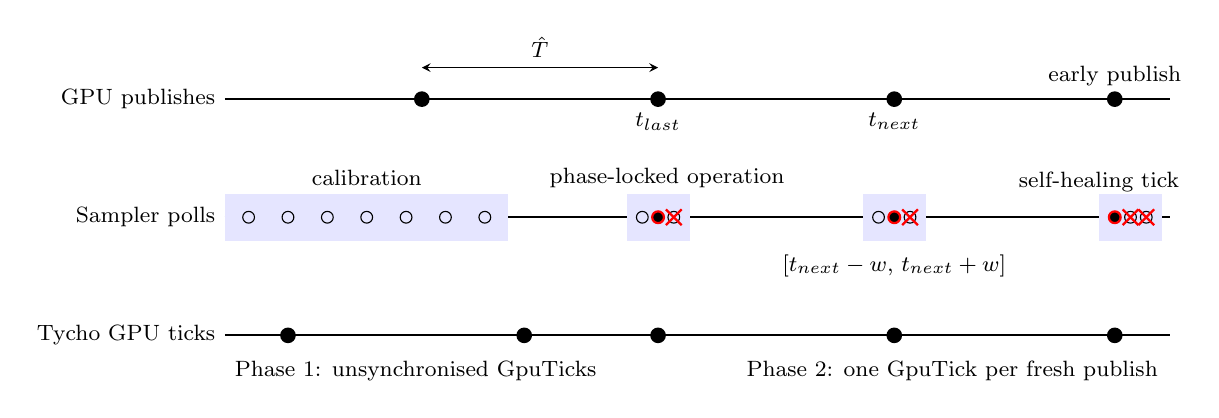
\begin{tikzpicture}[
    >=stealth,
    publish/.style={circle,fill=black,inner sep=2pt},
    poll-calib/.style={circle,draw=black,inner sep=1.5pt},
    poll-base/.style={circle,fill=black,inner sep=1.5pt},
    poll-burst/.style={circle,draw=black,inner sep=1.5pt},
    tick/.style={circle,fill=black,inner sep=2pt},
    timeline/.style={thick},
    label/.style={font=\footnotesize}
]

% Horizontal extents
\def\xmin{0}
\def\xmax{12}

% Y positions for the three lanes
\def\ygpu{3.2}
\def\ysampler{1.7}
\def\ytick{0.2}

% ------------------------------------------------------------------
% 1) GPU publish lane (ground truth)
% ------------------------------------------------------------------
\draw[timeline] (\xmin,\ygpu) -- (\xmax,\ygpu);
\node[label,anchor=east] at (\xmin,\ygpu) {GPU publishes};

% True publish events (roughly equidistant)
\foreach \x in {2.5,5.5,8.5,11.3} {
  \node[publish] at (\x,\ygpu) {};
}
\node[label,anchor=south] at (11.3,\ygpu+0.05) {early publish};

% Annotate approximate period between two publishes
\draw[<->] (2.5,\ygpu+0.4) -- node[label,above] {$\hat{T}$} (5.5,\ygpu+0.4);

% Mark t_last and t_next for illustration
\node[label,anchor=north] at (5.5,\ygpu-0.05) {$t_{\text{last}}$};
\node[label,anchor=north] at (8.5,\ygpu-0.05) {$t_{\text{next}}$};

% ------------------------------------------------------------------
% 2) Sampler lane (calibration + phase-locked polls with burst window)
% ------------------------------------------------------------------
\draw[timeline] (\xmin,\ysampler) -- (\xmax,\ysampler);
\node[label,anchor=east] at (\xmin,\ysampler) {Sampler polls};

% Calibration phase block (left)
\def\xcalibStart{0.0}
\def\xcalibEnd{3.6}
\fill[blue!10] (\xcalibStart,\ysampler-0.3) rectangle (\xcalibEnd,\ysampler+0.3);
\node[label] at ({0.5*(\xcalibStart+\xcalibEnd)},\ysampler+0.50) {calibration};

% Calibration-phase polls (irregular, more frequent)
\foreach \x in {0.3,0.8,1.3,1.8,2.3,2.8,3.3} {
  \node[poll-calib] at (\x,\ysampler) {};
}

% Burst-style windows around predicted publish times in phase-locked regime
\def\tpred{5.5}
\def\whalf{0.4}
\fill[blue!10] (\tpred-\whalf,\ysampler-0.3) rectangle (\tpred+\whalf,\ysampler+0.3);

\def\tpred{8.5}
\def\whalf{0.4}
\fill[blue!10] (\tpred-\whalf,\ysampler-0.3) rectangle (\tpred+\whalf,\ysampler+0.3);
\node[label,anchor=north] at (\tpred,\ysampler-0.35)
  {$[t_{\text{next}}-w,\,t_{\text{next}}+w]$};

\def\tpred{11.5}
\def\whalf{0.4}
\fill[blue!10] (\tpred-\whalf,\ysampler-0.3) rectangle (\tpred+\whalf,\ysampler+0.3);

% Phase-locked base polls: successful observation polls
\node[poll-base,draw=red,thick] at (5.5,\ysampler) {};
\node[poll-base,draw=red,thick] at (8.5,\ysampler) {};
% Last window: successful observation comes slightly early
\node[poll-base,draw=red,thick] at (11.3,\ysampler) {};
\node[label,anchor=south] at (11.1,\ysampler+0.2) {self-healing tick};

% Additional burst-mode polls around t_next (denser sampling inside window)
\foreach \x in {5.3,5.7,8.3,8.7,11.5,11.7} {
  \node[poll-burst] at (\x,\ysampler) {};
}

% Polls that get skipped AFTER a successful observation:
% - in the first two windows: the late burst poll
% - in the last window: the scheduled base poll at 11.5 and the late burst poll at 11.7
\foreach \x in {5.7,8.7,11.5,11.7} {
  \draw[red,thick] (\x-0.10,\ysampler-0.10) -- (\x+0.10,\ysampler+0.10);
  \draw[red,thick] (\x-0.10,\ysampler+0.10) -- (\x+0.10,\ysampler-0.10);
}

% Optional annotation: phase-locked region
\node[label,anchor=west] at (4.0,\ysampler+0.50) {phase-locked operation};

% ------------------------------------------------------------------
% 3) Tycho GPU tick lane (two phases)
% ------------------------------------------------------------------
\draw[timeline] (\xmin,\ytick) -- (\xmax,\ytick);
\node[label,anchor=east] at (\xmin,\ytick) {Tycho GPU ticks};

% Phase 1: same cadence as publishes, but not phase-aligned (during calibration)
\foreach \x in {0.8,3.8} {
  \node[tick] at (\x,\ytick) {};
}

% Phase 2: phase-locked, one tick per fresh device update
\foreach \x in {5.5,8.5,11.3} {
  \node[tick] at (\x,\ytick) {};
}

\node[label,anchor=west] at (0.0,\ytick-0.45)
  {Phase 1: unsynchronised \code{GpuTick}s};

\node[label,anchor=west] at (6.5,\ytick-0.45)
  {Phase 2: one \code{GpuTick} per fresh publish};

\end{tikzpicture}
\caption{Phase-aware GPU polling timeline}
\label{fig:gpu_phaseaware_timeline}
\end{figure}

\subsection{Event Lifecycle}
\label{subsec:gpu_event_lifecycle}

The GPU collector converts each confirmed hardware update into a
monotonically-timestamped \code{GpuTick} that integrates into Tycho’s
multi-domain energy timeline.  
The lifecycle consists of five stages: polling, device acquisition, optional
process acquisition, freshness detection, and tick emission.

\paragraph{1.\ Poll Initiation.}
Polling is triggered solely by the phase-aware scheduler
(\S~\ref{subsec:gpu_phaseaware_concept},
\S~\ref{subsec:gpu_phaseaware_math}).  
Base-mode polls track long-term cadence drift; burst-mode polls densely probe
the vicinity of predicted update edges.  
Each poll receives a monotonic timestamp $t_{\text{now}}$ that anchors the
resulting event.

\paragraph{2.\ Device Snapshot Acquisition.}
A poll retrieves device-level telemetry for all GPUs and MIG instances,
capturing power, utilisation, clocks, thermals, and memory state.  
All values reflect the device’s instantaneous condition at $t_{\text{now}}$ and
form a consistent cross-device snapshot of the accelerator subsystem.

\paragraph{3.\ Optional Process Snapshot Acquisition.}
If available, process-level telemetry is sampled over a backend-defined
wall-clock window (\S~\ref{subsec:gpu_process_window}).  
Although retrospective, these samples are associated with the same monotonic
timestamp as the device snapshot, ensuring that device and process data remain
correlated without temporal ambiguity.

\paragraph{4.\ Freshness Determination.}
The collector compares the new device snapshot with the most recent confirmed
update.  
Cumulative energy counters, when available, serve as the authoritative freshness
signal; otherwise Tycho uses a power-delta threshold to avoid counting noise as
updates.  
Only fresh snapshots update the period and phase estimators and proceed to the
next stage.

\paragraph{5.\ Tick Emission.}
A fresh observation is converted into a \code{GpuTick} containing device and
(optional) process snapshots and the timestamp $t_{\text{now}}$.  
The tick is then delivered to Tycho’s multi-domain ring buffer
(\S~\ref{subsec:ringbuffer_overview}).  
If no fresh update is detected, the poll produces no tick, ensuring that the GPU
timeline faithfully reflects the hardware’s publish cadence.

\paragraph{Summary.}
The event lifecycle ensures that GPU telemetry is sampled only when meaningful,
timestamped consistently with Tycho’s timebase, and integrated without blocking
or duplication.  
Each hardware update generates exactly one \code{GpuTick}, providing a precise,
causally ordered input to Tycho’s cross-domain energy attribution pipeline.

\subsection{Per-Process Telemetry Window}
\label{subsec:gpu_process_window}

Device-level metrics describe the instantaneous state of each GPU, but many
applications require attributing accelerator activity to individual processes or
containers.  
NVIDIA’s interfaces provide such information only in the form of \emph{aggregated
utilisation over a caller-specified time window}.  
Correctly selecting and interpreting this window is essential for obtaining
meaningful per-process data and for aligning process-level records with the
device-level timeline maintained by Tycho.

\paragraph{Wall-Clock Semantics.}
Unlike device publishes, which occur on the GPU’s internal cadence,
NVIDIA’s per-process APIs integrate utilisation over a duration supplied by the
caller.  
These interfaces expect a \emph{wall-clock} interval, expressed in milliseconds,
rather than a duration derived from Tycho’s monotonic timebase.  
The distinction is crucial: Tycho’s monotonic clock operates on an internal
quantum chosen to support high-resolution scheduling (\S~\ref{sec:tycho_timing_engine}),
but this quantum has no defined relationship to real elapsed time.  
Using monotonic differences directly would produce windows that are several
orders of magnitude too short, yielding incomplete utilisation samples.

For this reason, Tycho maintains a separate wall-clock origin for each GPU or
MIG instance.  
Whenever process telemetry is requested, the duration since the last successful
query is computed using wall-clock time, ensuring that the backend receives a
true real-time interval.

\paragraph{Window Derivation.}
For each owner (physical GPU or MIG instance), Tycho records the timestamp
$t^{(i)}_{\text{last}}$ of the most recent successful process query.  
When a new query occurs at time $t^{(i)}_{\text{now}}$, the raw duration
\[
  \Delta t^{(i)}_{\text{raw}} = t^{(i)}_{\text{now}} - t^{(i)}_{\text{last}}
\]
is transformed according to backend expectations:

\begin{enumerate}
  \item \emph{Clamping.}  
  The duration is restricted to a safe range  
  $\Delta t_{\min} \le \Delta t^{(i)} \le \Delta t_{\max}$  
  to avoid zero-length or excessively long sampling windows.  

  \item \emph{Millisecond granularity.}  
  NVIDIA’s process APIs accept durations in whole milliseconds.  
  Tycho therefore rounds the clamped value up to the next full millisecond to
  prevent systematic underestimation of utilisation.
\end{enumerate}

After a successful query, the wall-clock origin is updated to
$t^{(i)}_{\text{last}} \leftarrow t^{(i)}_{\text{now}}$, establishing continuity
across successive sampling windows.

\paragraph{Temporal Alignment with Device Updates.}
Even though per-process telemetry describes accumulated activity rather than a
snapshot, Tycho ensures that all process samples remain aligned with the device
timeline.  
Each process record is associated with the device-level timestamp of the poll
that triggered the query.  
If a device has never produced a fresh update, the collector uses the timestamp
of the most recent device tick as the initial origin for its process window.
This guarantees that device and process metrics are linked to the same global
temporal reference and can be fused without interpolation.

\paragraph{Backend Variability and Robustness.}
Process-level support varies widely across NVIDIA hardware and software stacks.
DCGM-capable systems typically expose high-quality, high-resolution utilisation
data, whereas NVML-only systems (particularly consumer GPUs) may provide limited
or noisy information.  
Tycho’s design accommodates these differences gracefully: when a process query
fails, the wall-clock origin is still advanced to prevent tight retry loops, and
device-level sampling proceeds unaffected.  
This ensures stable behaviour even in mixed configurations where only a subset
of devices expose meaningful per-process telemetry.

\paragraph{Summary.}
By separating wall-clock process windows from monotonic device timestamps and
carefully aligning both within Tycho’s timing architecture, the GPU collector
provides process-level telemetry that is semantically correct, temporally
consistent, and robust to backend limitations.  
This separation of concerns is essential for accurate multi-tenant attribution in
heterogeneous accelerator environments.

\subsection{Collected Metrics}
\label{subsec:gpu_metrics}

The GPU collector reports two complementary categories of telemetry that together
describe both the instantaneous state of each accelerator and the distribution
of GPU activity across processes.  
All metrics are incorporated into a unified \code{GpuTick} structure and
timestamped under Tycho’s monotonic timebase, ensuring direct comparability with other domains.

\paragraph{Device-Level Metrics.}
Device and MIG-level metrics capture the operational state of the accelerator at
the moment Tycho detects a fresh hardware update.  
These values include power, utilisation, memory usage, thermal data, and clock
frequencies, along with backend-specific fields such as instantaneous power
samples or cumulative energy counters.  
Cumulative energy, when available, is used as the authoritative indicator of
publish boundaries and therefore plays a central role in the timing model and
freshness detection. Due to a tendency of NVIDIA GPUs to still produce (invalid) values when queried for cumulative energy, the actual availability of correct cumulative energy-metrics is verified during the initial calibration.

\paragraph{Process-Level Metrics.}
Process-level metrics describe the aggregated utilisation of individual
processes over the backend-defined wall-clock window
(\S~\ref{subsec:gpu_process_window}).  
They enable multi-tenant attribution by associating GPU activity with specific
applications, containers, or pods.  
Because these values represent accumulated work rather than an instantaneous
snapshot, they are paired with the device-level timestamp of the triggering
poll, ensuring temporal consistency within Tycho’s unified timeline.

Tables~\ref{tab:gpu-device-metrics} and~\ref{tab:gpu-process-metrics} summarise
the metrics collected at both levels.

\begin{table}[H]
\centering
\small
\begin{tabular}{p{3.5cm} p{0.7cm} p{8.8cm}}
\toprule
\textbf{Metric} & \textbf{Unit} & \textbf{Description} \\
\midrule
\multicolumn{3}{l}{\textit{Utilisation metrics}} \\[2pt]
\code{SMUtilPct}      & \%   & Streaming multiprocessor (SM) utilisation. \\
\code{MemUtilPct}     & \%   & Memory controller utilisation. \\
\code{EncUtilPct}     & \%   & Hardware video encoder utilisation. \\
\code{DecUtilPct}     & \%   & Hardware video decoder utilisation. \\[4pt]

\multicolumn{3}{l}{\textit{Energy and thermal metrics}} \\[2pt]
\code{PowerMilliW}        & mW & Instantaneous power via NVML/DCGM (1s average). \\
\code{InstantPowerMilliW} & mW & High-frequency instantaneous power from NVIDIA field APIs. \\
\code{CumEnergyMilliJ}    & mJ & Cumulative energy counter (preferred freshness signal). \\
\code{TempC}              & °C & GPU temperature. \\[4pt]

\multicolumn{3}{l}{\textit{Memory and frequency metrics}} \\[2pt]
\code{MemUsedBytes}   & bytes & Allocated framebuffer memory. \\
\code{MemTotalBytes}  & bytes & Total framebuffer memory. \\
\code{SMClockMHz}     & MHz   & SM clock frequency. \\
\code{MemClockMHz}    & MHz   & Memory clock frequency. \\[4pt]

\multicolumn{3}{l}{\textit{Topology and metadata}} \\[2pt]
\code{DeviceIndex}    & --    & Numeric device identifier. \\
\code{UUID}           & --    & Stable device UUID. \\
\code{PCIBusID}       & --    & PCI bus identifier. \\
\code{IsMIG}          & --    & Indicates a MIG instance. \\
\code{MIGParentID}    & --    & Parent device index for MIG instances. \\
\code{Backend}        & --    & Backend type (\code{NVML} or \code{DCGM}). \\
\bottomrule
\end{tabular}
\caption{Device- and MIG-level metrics collected by the GPU subsystem.}
\label{tab:gpu-device-metrics}
\end{table}

\begin{table}[H]
\centering
\small
\begin{tabular}{p{3.5cm} p{0.7cm} p{8.8cm}}
\toprule
\textbf{Metric} & \textbf{Unit} & \textbf{Description} \\
\midrule
\code{Pid}              & --   & Process identifier. \\
\code{ComputeUtil}      & \%   & Per-process SM utilisation aggregated over the query window. \\
\code{MemUtil}          & \%   & Per-process memory controller utilisation. \\
\code{EncUtil}          & \%   & Per-process encoder utilisation. \\
\code{DecUtil}          & \%   & Per-process decoder utilisation. \\[4pt]

\code{GpuIndex}         & --   & Device or MIG instance to which the sample belongs. \\
\code{GpuUUID}          & --   & Corresponding device UUID. \\
\code{TimeStampUS}      & µs   & Backend timestamp associated with the utilisation record. \\[4pt]

\multicolumn{3}{l}{\textit{MIG metadata (when applicable)}} \\[2pt]
\code{GpuInstanceID}     & --  & MIG GPU instance identifier. \\
\code{ComputeInstanceID} & --  & MIG compute-instance identifier. \\
\bottomrule
\end{tabular}
\caption{Process-level metrics collected over a backend-defined time window.}
\label{tab:gpu-process-metrics}
\end{table}

\subsection{Configuration Parameters}
\label{subsec:gpu_config}

The GPU collector exposes only a minimal set of configuration parameters.  
In contrast to traditional monitoring systems that require hand-tuned polling
intervals, Tycho derives the parameters of the phase-aware sampler directly from
the engine cadence calibrated during system startup
(\S~\ref{sec:tycho_timing_engine}).  
This ensures that GPU sampling inherits the same temporal consistency as all
other energy domains and remains robust across heterogeneous hardware.

The configuration governs three tightly coupled aspects of the sampling
mechanism:

\begin{itemize}
  \item \textbf{Cadence bounds.}  
  The initial estimate of the GPU publish period, as well as its minimum and
  maximum permissible values, are expressed as simple fractions of the engine
  cadence.  
  This constrains the period estimator to a stable range without relying on
  device-specific heuristics.

  \item \textbf{Polling intervals.}  
  Both base-mode and burst-mode polling frequencies are derived from fixed
  ratios of the engine cadence.  
  As a result, Tycho polls aggressively only when a publish is predicted without requiring manual tuning.

  \item \textbf{Burst-window width.}  
  The half-width of the burst window around $t_{\text{next}}$ is likewise tied
  to the engine cadence.  
  This determines how narrowly the sampler focuses its hyperpolling effort
  around predicted publish edges.
\end{itemize}

Because all parameters scale with the calibrated cadence, the sampler adapts
automatically to different GPU generations, backend behaviours, and platform
timing characteristics.  
No user-facing configuration is required; temporal correctness follows directly
from Tycho’s system-wide timing model.


\subsection{Robustness and Limitations}
\label{subsec:gpu_limitations}

The GPU collector is designed to operate reliably across heterogeneous hardware,
backend capabilities, and driver behaviours.  
Its phase-aware sampling, decoupled event queue, and unified timebase ensure
that GPU telemetry integrates cleanly with Tycho’s multi-domain measurement
framework.  
Nevertheless, several structural constraints in NVIDIA’s telemetry ecosystem
define the practical limits of what can be inferred and with what temporal
precision.

\paragraph{Backend Variability.}
The capabilities of \code{NVML} and \code{DCGM} differ significantly across GPU
generations and product classes.  
Datacenter GPUs typically expose cumulative energy counters, high-frequency
instant power fields, and stable process-level utilisation, while consumer GPUs
often lack cumulative energy and provide only coarse utilisation metrics.  
Tycho handles these differences gracefully (sampling continues even when certain
fields are missing) but the quality of the resulting attribution reflects the
capabilities of the underlying hardware.

\paragraph{Power Measurement Limitations.}
The widely used \code{nvmlDeviceGetPowerUsage} call provides a \emph{one-second
trailing average}, which is unsuitable as a high-frequency power signal.  
Tycho therefore relies on instantaneous power fields (e.g.\ field~186) when
available, and uses cumulative energy counters as the authoritative freshness
indicator.  
On devices lacking both instantaneous fields and cumulative energy, power-based
freshness detection becomes less precise, increasing uncertainty in the inferred
publish cadence.

\paragraph{Process Attribution Constraints.}
Process-level utilisation is inherently aggregated over a wall-clock window,
since NVIDIA provides no access to per-process instantaneous state.  
This retrospective design imposes two limitations: (i) spikes shorter than the
sampling window may be attenuated, and (ii) per-process values cannot be aligned
to the exact moment of a device publish.  
Tycho addresses this by using the device-level timestamp to anchor all process
records, but the granularity of attribution ultimately depends on backend
resolution.

\paragraph{Cadence Inference and Jitter.}
Because the driver does not expose its publish cadence, Tycho must infer it
indirectly.  
Under conditions of high load, thermal transitions, or DVFS-induced jitter,
publish intervals may vary, introducing uncertainty into edge prediction.
Tycho’s EMA-based estimators maintain stability under such variability, but
prediction accuracy is inherently bounded by the noisiness of the underlying
telemetry.

\paragraph{Mixed and MIG Configurations.}
Systems combining MIG and non-MIG devices, or devices with partial telemetry
support, may expose inconsistent field availability across accelerators.  
Cumulative energy counters may exist for some instances but not others; process
information may be available only at the parent-device level.  
Tycho handles these cases through per-device fallbacks and independent cadence
models, but the precision of multi-GPU attribution varies with the fidelity of
each device’s telemetry.

\paragraph{Vendor support scope.} The current GPU collector supports only NVIDIA-based accelerators, following the design of Kepler. While this excludes other vendors, it is justifiable: according to market research\parencite{YoleGroup2025DataCenterSemiconductorTrends}, NVIDIA captured approximately 93\% of the server GPU revenue in 2024. Given this dominant share, focusing on NVIDIA hardware is acceptable for the majority of data-centre GPU deployments.

% \section{RAPL Collector Integration}
\label{sec:rapl_collector}

\subsection{Purpose and Scope}
\label{subsec:rapl_purpose}

The RAPL collector provides cumulative energy readings for all CPU related domains supported by the hardware.  
It retrieves these values once per tick and stores them in Tycho’s ring buffer without applying intermediate processing.  
All interpretation, differencing, and model level handling occur in the downstream analysis layer.

\subsection{Collector Mechanics and Data Flow}
\label{subsec:rapl_mechanics}

At each tick the collector is invoked by the timing engine to obtain a complete snapshot of the RAPL domains for all sockets.  
The collector queries the shared RAPL component, which exposes the cumulative hardware counters for package, core, uncore, and memory related domains when available.  
The results are placed into a \code{RaplTick} structure containing a monotonic timestamp and a per socket map of domain counters.

Only raw cumulative values are stored.  
The collector does not compute differences, apply scaling, or perform validity checks beyond verifying that the system exposes RAPL counters.  
Domain availability is determined by the underlying hardware, and unsupported domains are omitted from the per socket map.  
Each tick therefore contains exactly one set of cumulative counters per socket for all domains supported by that platform.

The resulting \code{RaplTick} is immutable and is written directly into Tycho’s ring buffer, where it becomes available to the attribution and export components.

\subsection{Exported Metrics}
\label{subsec:rapl_metrics}

The metrics exported by the RAPL collector are shown in
Table~\ref{tab:rapl-metrics}.  
All values represent cumulative energy since a hardware defined starting point and are reported once per tick.

\begin{table}[H]
\centering
\small
\begin{tabular}{p{3.5cm} p{0.9cm} p{8.6cm}}
\toprule
\textbf{Metric} & \textbf{Unit} & \textbf{Description} \\
\midrule
\multicolumn{3}{l}{\textit{Per-socket energy counters}} \\[4pt]
\code{Pkg}    & mJ & Cumulative package energy per socket\newline(RAPL \code{PKG} domain). \\
\code{Core}   & mJ & Cumulative core energy per socket\newline (RAPL \code{PP0} domain), when available. \\
\code{Uncore} & mJ & Cumulative uncore energy per socket\newline (RAPL \code{PP1} or uncore domain), when available. \\
\code{DRAM}   & mJ & Cumulative DRAM energy per socket\newline (RAPL \code{DRAM} domain), if the platform exposes it. \\[6pt]

\multicolumn{3}{l}{\textit{Metadata}} \\[4pt]
\code{Source}    & -- & Identifier of the active RAPL backend (for example \code{powercap})\\
\code{Sockets}   & -- & Map from socket identifier to the corresponding set of domain counters. \\
\code{SampleMeta.Mono} & -- & Monotonic timestamp assigned by Tycho's timing engine at the moment of collection. \\
\bottomrule
\end{tabular}
\caption{Metrics exported by the RAPL collector per \code{RaplTick}.}
\label{tab:rapl-metrics}
\end{table}

\subsection{Stability and Platform Variability}
\label{subsec:rapl_stability}

The collector records only the domains exposed by the hardware.  
Some platforms provide package level counters only, whereas others additionally expose core, uncore, or memory related domains.  
The collector does not approximate or reconstruct unsupported domains and stores only the counters returned by the system.

The cumulative counters obtained from RAPL are stable at the tick interval used by Tycho and do not exhibit missing data or inconsistent increments at this scale.  
Since the collector performs no differencing, scaling, or interpolation, it remains minimal and does not introduce additional sources of variability.

\subsection{Limitations}
\label{subsec:rapl_limitations}

Limitations of the RAPL collector arise solely from platform specific domain availability.  
Platforms that do not provide a particular domain omit it from the exported tick.  
Beyond these hardware differences the collector has no additional constraints, and all further processing occurs in the downstream analysis layer.


% \section{RAPL Collector Integration}
% \label{sec:rapl_collector}

% \subsection{Scope and Baseline}
% \label{subsec:rapl_scope}

% RAPL-based telemetry provides CPU energy readings at the level of logical power domains such as package, cores, uncore, and DRAM.  
% Tycho reuses Kepler's existing RAPL implementation almost unchanged: discovery, scaling, and raw counter reads are still provided by the shared \code{components} package (via the \code{power}-interface), which wraps the kernel's \code{powercap} interface and related mechanisms.  
% This collector therefore does not introduce a new hardware access path but instead focuses on integrating the existing RAPL metrics into Tycho's timing and buffering model.

% \subsection{Architecture and Data Flow}
% \label{subsec:rapl_architecture}

% The collector is deliberately simple and stateless.  
% On each engine tick, the \code{Collect} function:

% \begin{enumerate}
%   \item Verifies that system-wide RAPL collection is supported via\newline \code{components.IsSystemCollectionSupported()}.
%   \item Obtains a snapshot of cumulative energy counters for all sockets and domains through \code{components.GetAbsEnergyFromNodeComponents()}.
%   \item Translates the per-socket results into a \code{RaplTick} structure containing:
%   \begin{itemize}
%     \item a monotonic timestamp derived from \code{clock.Mono}, and
%     \item a map from socket identifier to domain counters.
%   \end{itemize}
%   \item Pushes exactly one immutable \code{RaplTick} into the shared ring buffer.
% \end{enumerate}

% The tick stores raw, monotonically increasing counters in millijoules rather than precomputed deltas.  
% Downstream analysis components compute inter-tick differences, perform wraparound handling, and align RAPL energy with CPU activity and platform-level power traces.  
% This separation keeps the collector minimal while allowing the analysis layer to apply a consistent attribution strategy across all energy domains.

% \subsection{Collected Metrics}
% \label{subsec:rapl_metrics}

% Table~\ref{tab:rapl-metrics} summarises the metrics stored in each \code{RaplTick}.\\  
% All counters are subject to platform availability.

% \begin{table}[H]
% \centering
% \small
% \begin{tabular}{p{3.5cm} p{0.9cm} p{8.6cm}}
% \toprule
% \textbf{Metric} & \textbf{Unit} & \textbf{Description} \\
% \midrule
% \multicolumn{3}{l}{\textit{Per-socket energy counters}} \\[4pt]
% \code{Pkg}    & mJ & Cumulative package energy per socket\newline(RAPL \code{PKG} domain). \\
% \code{Core}   & mJ & Cumulative core energy per socket\newline (RAPL \code{PP0} domain), when available. \\
% \code{Uncore} & mJ & Cumulative uncore energy per socket\newline (RAPL \code{PP1} or uncore domain), when available. \\
% \code{DRAM}   & mJ & Cumulative DRAM energy per socket\newline (RAPL \code{DRAM} domain), if the platform exposes it. \\[6pt]

% \multicolumn{3}{l}{\textit{Metadata}} \\[4pt]
% \code{Source}    & -- & Identifier of the active RAPL backend (for example \code{powercap})\\
% \code{Sockets}   & -- & Map from socket identifier to the corresponding set of domain counters. \\
% \code{SampleMeta.Mono} & -- & Monotonic timestamp assigned by Tycho's timing engine at the moment of collection. \\
% \bottomrule
% \end{tabular}
% \caption{Metrics exported by the RAPL collector per \code{RaplTick}.}
% \label{tab:rapl-metrics}
% \end{table}

% These metrics provide a compact, hardware-backed view of CPU and memory-subsystem energy at socket granularity.  
% Combined with the timing guarantees of Tycho's engine and ring buffer, they form the CPU-related energy baseline against which per-process activity and platform-level power are later correlated.

% \subsection{Limitations and Reuse}
% \label{subsec:rapl_limitations}

% Because RAPL domain availability is hardware dependent, not all fields in
% Table~\ref{tab:rapl-metrics} are present on every platform.  
% Some systems expose only package-level counters, while others additionally
% provide core, uncore, or DRAM domains.  
% The collector reports only what the hardware exposes and does not attempt to
% approximate or reconstruct missing values.

% Beyond this domain variability, no further limitations apply.  
% The collector is intentionally minimal and serves as a timing-aware wrapper
% around the raw counters, providing reliable cumulative energy readings without
% adding intermediate modelling or transformation.

% \section{Redfish Collector Integration}
\label{sec:redfish_collector}

The Redfish collector retrieves node-level power measurements from the server's
Baseboard Management Controller (BMC) through the Redfish API.  As an
out-of-band source, it complements in-band telemetry such as RAPL by providing a
hardware-validated view of total chassis power.  Tycho integrates these
measurements into its global timing framework, ensuring that BMC-sourced data
can be correlated with all other collectors using a common monotonic clock.

\subsection{Overview and Objectives}
\label{subsec:redfish_overview}

Redfish power readings are updated asynchronously and often with vendor-specific
timing behaviour.  
Tycho therefore focuses on robustness, controlled polling, and precise
timestamping rather than high-frequency sampling.  The collector executes a
single BMC query at the global engine cadence, extracts the current chassis
power value, and emits a sample only when necessary.  All readings are
timestamped with Tycho's monotonic timebase and annotated with freshness
metadata to express their temporal accuracy.

\subsection{Baseline in Kepler}
\label{subsec:redfish_baseline}

Kepler's original Redfish integration consisted of a periodic background ticker
that queried the BMC at fixed intervals, typically every sixty seconds.  It
retrieved only instantaneous chassis power and made no distinction between new
and repeated measurements.  No mechanism existed to detect stale data, associate
readings with BMC timestamps, or align Redfish values with other collectors.
The Redfish implementation was therefore sufficient for coarse system-power
reporting, but not suitable for the finer temporal structure required by Tycho.

\subsection{Refactoring and Tycho Extensions}
\label{subsec:redfish_refactor}

\subsubsection{Timing Ownership and Polling Control}
\label{subsubsec:redfish_timing}

Tycho removes Kepler's internal Redfish ticker entirely.  
Polling is performed exclusively by Tycho's global timing engine, which invokes
the collector once per engine tick.  This ensures that all Redfish interactions
occur in lockstep with the rest of the measurement pipeline and that every
sample can be aligned unambiguously with simultaneous energy and utilization
values from other collectors.

The polling frequency itself is never altered by the Redfish collector.
Tycho maintains deterministic, externally selected polling intervals regardless
of BMC behaviour.

\subsubsection{Sequence-Based Newness Detection}
\label{subsubsec:redfish_newness}

Many BMCs return identical payloads for extended periods and only publish new
power values intermittently.  To avoid emitting redundant samples, Tycho uses a
per-chassis sequence number provided by the Redfish client.  Each measurement is considered fresh only when this sequence number differs from the one observed in the previous engine tick.

No header-based (for example \code{ETag}) or value-delta heuristics are used.
Newness is driven solely by this explicit sequence value, ensuring a consistent
and vendor-agnostic update mechanism.

\subsubsection{Heartbeat Mechanism and Freshness Metric}
\label{subsubsec:redfish_heartbeat}

Because BMC refresh cycles can be irregular, Tycho maintains a heartbeat window
for each chassis.  If no new Redfish sample has appeared within this window, the
collector emits a heartbeat sample that carries forward the last known power
value.  This prevents gaps in the power time series while avoiding unnecessary
fabrication of data.

Each emitted sample includes a freshness metric, defined as the time difference
between the BMC-reported timestamp (when available) and the local collection time.  This value quantifies the latency of the underlying Redfish pipeline.  
Freshness does not influence newness detection; it is an informational quality
indicator for the analysis layer.

\subsubsection{Fixed vs Auto Heartbeat Mode}
\label{subsubsec:redfish_autopoll}

Tycho supports two Redfish operating modes, selected by
\code{TYCHO\_REDFISH\_POLL\_AUTOTUNE}.  Both modes perform BMC polling strictly
at the global engine cadence.

In fixed mode, the heartbeat window is defined entirely by the user through
\code{TYCHO\_REDFISH\_HEARTBEAT\_MS}.  
This guarantees deterministic behaviour and is appropriate for reproducible
benchmarks.

In auto mode, Tycho adapts the heartbeat window to the BMC's observed update
pattern.  
Whenever a fresh sequence number is detected, the collector measures the
inter-arrival duration to the previous update and stores it in a sliding window.
The median of this window is taken as the representative publication period, and
the heartbeat timeout is set to approximately \(1.5\) times this value, clamped
between conservative bounds.  
This technique aligns Tycho's emission behaviour with the hardware's natural
update rhythm while retaining deterministic polling.

\subsection{Collected Metrics}
\label{subsec:redfish_metrics}

The Redfish collector emits one record per chassis whenever a new measurement is detected or a heartbeat event occurs.  Each record is timestamped using Tycho's monotonic clock and annotated with metadata relevant for temporal correlation.
Table~\ref{tab:redfish-metrics} summarises the collected fields.

\begin{table}[h]
\centering
\begin{tabular}{p{3cm} p{1cm} p{9cm}}
\toprule
\textbf{Metric} & \textbf{Unit} & \textbf{Description} \\
\midrule
\multicolumn{3}{l}{\textit{Primary power metric}} \\[4pt]
\code{PowerWatts} & W & Instantaneous chassis power reported by the BMC. \\[4pt]

\multicolumn{3}{l}{\textit{Temporal and identity metadata}} \\[4pt]
\code{ChassisID} & - & Identifier of the chassis or enclosure. \\
\code{Seq} & - & Server-provided sequence number indicating new measurements. \\
\code{SourceTime} & s & Timestamp provided by the BMC, if available. \\
\code{CollectorTime} & s & Local collection time of the measurement. \\
\code{FreshnessMs} & ms & Difference between \code{SourceTime} and \code{CollectorTime}. \\
\bottomrule
\end{tabular}
\caption{Metrics collected by the Redfish collector.}
\label{tab:redfish-metrics}
\end{table}

Energy values such as \code{EnergyMilliJ} are computed downstream by integrating the power series and are not directly produced by the collector.

\subsection{Integration and Data Flow}
\label{subsec:redfish_integration}

The Redfish collector is a passive component within Tycho's unified collection
pipeline.  At each engine tick it performs one BMC query, evaluates newness and
heartbeat conditions, attaches monotonic timestamps, and writes the resulting
record into a synchronized ring buffer.  
No additional processing occurs within the collector; all energy computations
and correlations across metrics are performed in Tycho's analysis stage.

\subsection{Accuracy and Robustness Improvements}
\label{subsec:redfish_accuracy}

Tycho improves Redfish robustness by combining explicit sequence-based newness
tracking, adaptive heartbeat windows, and freshness estimation.  
Sequence tracking ensures that repeated BMC responses do not produce redundant
samples.  
Adaptive heartbeat windows accommodate BMCs with slow or irregular update
cycles.  
Freshness metadata exposes the latency of Redfish timestamps, allowing the
analysis layer to assess the temporal reliability of each reading.

These measures provide stable and chronologically consistent power telemetry
across heterogeneous BMC implementations.

\subsection{Limitations}
\label{subsec:redfish_limitations}

Redfish sampling remains limited by the update rate and timestamp quality of the underlying BMC.  Most implementations refresh power data at intervals on the order of one to two seconds.  Redfish does not report component-level power
breakdowns; only total chassis power is available.  For fine-grained
attribution, Tycho relies on complementary in-band collectors such as RAPL and
eBPF.

% \section{Configuration Management}
\label{subsec:tycho_config}

\subsection{Overview and Role in the Architecture}
\label{subsubsec:tycho_config_overview}

Tycho adopts a simple, centralized configuration layer that is initialized during exporter startup and made globally accessible through typed structures.
This layer defines all runtime parameters controlling timing, collection, and analysis behaviour.
It serves as the interface between user-defined settings and the internal scheduling and buffering logic described in \S~\ref{sec:tycho_timing_engine}.

The configuration is loaded once at startup, combining defaults, environment variables, and optional overrides passed through Helm or local flags.
Its purpose is not to support dynamic reconfiguration, but to provide deterministic, reproducible operation across (experimental) runs.
No backward compatibility with previous Kepler versions is maintained.

\subsection{Configuration Sources}
\label{subsubsec:tycho_config_sources}

Configuration values can be provided in three ways:
first, through a \code{values.yml} file during Helm installation,
second, as command-line flags for local or debugging builds,
and third, via predefined environment variables that act as defaults.

During startup, Tycho sequentially evaluates these sources in fixed order—
defaults are loaded first, then environment variables,
followed by any user-supplied overrides.
The resulting configuration is stored in memory and printed once for verification.
After initialization, all components reference the same in-memory configuration,
ensuring consistent behaviour across collectors and analysis modules.

\subsection{Implementation and Environment Variables}
\label{subsubsec:tycho_config_env}
The configuration implementation in Tycho closely follows the approach used in Kepler~v0.9.0.
Each configuration key is mapped to an environment variable, which is resolved at startup through dedicated lookup functions.
If no variable is set, the corresponding default value is applied.
This mechanism enables flexible configuration without external dependencies or complex parsing logic.
All variables are read once during initialization, after which they are cached in typed configuration structures.
This guarantees consistent operation even if environment variables change later, since Tycho is not designed for live reconfiguration.
The configuration layer is invoked before the collectors and timing engine are instantiated,
ensuring that parameters such as polling intervals, buffer sizes, or analysis triggers are available to all components from the first cycle onward.

\subsubsection{Validation and Normalization at Startup}
\label{subsubsec:tycho_config_validate}

During initialization, Tycho validates all user inputs and normalizes them to a consistent, safe configuration.
First, basic bounds are enforced: the global timebase quantum must be positive, non-negative values are required for all periods and delays, and missing essentials fall back to minimal defaults.
Trigger coherence is then checked. If \code{redfish} is selected while the Redfish collector is disabled, Tycho switches to the timer trigger and ensures a valid interval. Unknown triggers default to \code{timer}.

All periods and delays are aligned to the global quantum so that scheduling, buffering, and analysis operate on a common time grid.
The analysis wait \code{DelayAfterMs} is raised if needed to cover the longest enabled per-source delay.
Buffer sizing is derived from the slowest effective acquisition path (poll period plus delay) and the analysis wait, with a small safety margin.
If Redfish is enabled, its heartbeat requirement is included to guarantee coverage.
Sanity checks also ensure plausible Redfish cadence and warn if no collectors are enabled.
Non-fatal environment hints (for example the RAPL powercap path) are reported at low verbosity.

The result is a single, internally consistent configuration snapshot.
Adjustments are announced once at startup to aid reproducibility while avoiding log noise.

\subsection{Evolution in Newer Kepler Versions}
\label{subsubsec:tycho_config_evolution}

Subsequent Kepler releases (v0.10.0 and later) have replaced the environment-variable system with a unified configuration interface based on CLI flags and YAML files.
This modernized approach simplifies configuration management and aligns better with Kubernetes conventions, providing clearer defaults and validation at startup.

Tycho intentionally retains the v0.9.0 model to maintain structural continuity with its experimental foundation.
Since configuration handling is not a research focus, adopting the newer scheme would add complexity without scientific benefit.
Nevertheless, the newer Kepler design confirms that Tycho’s configuration logic can be migrated with minimal effort if long-term maintainability becomes a requirement.

\subsection{Available Parameters}
\label{subsubsec:tycho_config_parameters}

All parameters are read at startup and remain constant throughout execution.
The following table~\ref{tab:tycho_config_parameters} summarizes the user-facing configuration variables with their default values and functional scope.
Internal or experimental parameters are omitted for clarity.


XXXXXXXXXXXXXXXXXXXXXXXXXXXXXXXXXXXXXXXXXXXXXXXXXXXXXXXXXXXXXXXXXXXXXXXXXXXXXXXXXXXXXXXXXXXXXXXXXXXXXXXXXXXXXXXXXXXXXXXXXXXXXXXXXXXXXXXXXXXXXXXXXXXXXX
CHECK THIS TABLE BEFORE HANDIN, THIS NEEDS CLEANUP\\
XXXXXXXXXXXXXXXXXXXXXXXXXXXXXXXXXXXXXXXXXXXXXXXXXXXXXXXXXXXXXXXXXXXXXXXXXXXXXXXXXXXXXXXXXXXXXXXXXXXXXXXXXXXXXXXXXXXXXXXXXXXXXXXXXXXXXXXXXXXXXXXXXXXXXX
\begin{table}[h]
\centering
\tiny
\begin{tabular}{p{4.8cm} p{1.2cm} p{7cm}}
\toprule
\textbf{Variable} & \textbf{Default} & \textbf{Description} \\
\midrule
\multicolumn{3}{l}{\textit{Collector enable flags}} \\[4pt]
\code{TYCHO\_COLLECTOR\_ENABLE\_BPF} & \code{true} & Enables eBPF-based process metric collection. \\
\code{TYCHO\_COLLECTOR\_ENABLE\_RAPL} & \code{true} & Enables RAPL energy counter collection. \\
\code{TYCHO\_COLLECTOR\_ENABLE\_GPU} & \code{true} & Enables GPU power telemetry collection. \\
\code{TYCHO\_COLLECTOR\_ENABLE\_REDFISH} & \code{true} & Enables Redfish-based BMC power collection. \\[4pt]

\multicolumn{3}{l}{\textit{Timing and delays}} \\[4pt]
\code{TYCHO\_TIMEBASE\_QUANTUM\_MS} & \code{1} & Base system quantum (ms) defining the global monotonic time grid. \\
\code{TYCHO\_RAPL\_POLL\_MS} & \code{50} & RAPL polling interval (ms). \\
\code{TYCHO\_GPU\_POLL\_MS} & \code{200} & GPU telemetry polling interval (ms). \\
\code{TYCHO\_REDFISH\_POLL\_MS} & \code{1000} & Redfish polling interval (ms); should be below BMC publish cadence. \\
\code{TYCHO\_RAPL\_DELAY\_MS} & \code{0} & Expected delay between workload change and RAPL visibility (ms). \\
\code{TYCHO\_GPU\_DELAY\_MS} & \code{200} & Expected delay between workload change and GPU visibility (ms). \\
\code{TYCHO\_REDFISH\_DELAY\_MS} & \code{0} & Expected delay between workload change and Redfish visibility (ms). \\
\code{TYCHO\_REDFISH\_HEARTBEAT\_MAX\_GAP\_MS} & \code{3000} & Maximum tolerated gap between consecutive Redfish samples (ms). \\[4pt]

\multicolumn{3}{l}{\textit{Autotuning controls}} \\[4pt]
\code{TYCHO\_RAPL\_POLL\_AUTOTUNE} & \code{true} & Enables automatic calibration of RAPL polling interval. \\
\code{TYCHO\_RAPL\_DELAY\_AUTOTUNE} & \code{true} & Enables automatic calibration of RAPL delay. \\
\code{TYCHO\_GPU\_POLL\_AUTOTUNE} & \code{true} & Enables automatic calibration of GPU polling interval. \\
\code{TYCHO\_GPU\_DELAY\_AUTOTUNE} & \code{true} & Enables automatic calibration of GPU delay. \\
\code{TYCHO\_REDFISH\_POLL\_AUTOTUNE} & \code{true} & Enables automatic calibration of Redfish polling interval. \\
\code{TYCHO\_REDFISH\_DELAY\_AUTOTUNE} & \code{true} & Enables automatic calibration of Redfish delay. \\[4pt]

\multicolumn{3}{l}{\textit{Analysis parameters}} \\[4pt]
\code{TYCHO\_ANALYSIS\_TRIGGER} & \code{"timer"} & Defines analysis trigger: \code{redfish} or \code{timer}. \\
\code{TYCHO\_ANALYSIS\_EVERY\_SEC} & \code{15} & Interval for timer-based analysis (s). \\
\code{TYCHO\_ANALYSIS\_DETECT\_LONGEST\_DELAY} & \code{false} & Enables detection of the longest observed metric delay. \\
\bottomrule
\end{tabular}
\caption{User-facing configuration variables available in Tycho.}
\label{tab:tycho_config_parameters}
\end{table}

In summary, Tycho’s configuration layer provides a single, immutable snapshot of
all timing, polling, and analysis parameters.  
It is loaded once at startup, validated, normalized to a shared timebase, and
propagated to all collectors and analysis modules.  
The design prioritizes reproducibility and correctness: no live reconfiguration
is supported, and all behaviour is derived from explicit user input or well-defined
defaults.  
This central configuration snapshot ensures that the timing engine, collectors,
and buffering subsystem operate in a coherent, predictable manner throughout the
entire runtime.

% \section{Timing Engine}
\label{sec:tycho_timing_engine}

\subsection{Overview and Motivation}
\label{subsec:tycho_timing_overview}

Tycho introduces a dedicated timing engine that replaces the synchronous update loop used in Kepler with an event-driven, per-metric scheduling layer.  
While the conceptual motivation for this change was discussed in \S~\ref{sec:theoretical_timing}, its practical purpose is straightforward: to decouple the collection frequencies of heterogeneous telemetry sources and to establish a common temporal reference for subsequent analysis.

Each collector in Tycho (e.g., RAPL, eBPF, GPU, Redfish) operates under its own polling interval and is triggered by an aligned ticker maintained by the timing engine.  
All tickers share a single epoch (base timestamp) and are aligned to a configurable time quantum, ensuring deterministic phase relationships and bounded drift across all metrics.  
This architecture allows high-frequency sources to capture fine-grained temporal variation while preserving coherence with slower metrics.

The timing engine thus provides the temporal backbone of Tycho: it defines *when* each collector produces samples and ensures that all samples can later be correlated on a unified, monotonic timeline.  
Collected samples are pushed immediately into per-metric ring buffers, described in \S~\ref{sec:ringbuffer}, which retain recent histories for downstream integration and attribution.

\subsection{Architecture and Design}
\label{subsec:tycho_timing_design}

The timing engine is implemented in the \code{engine.Manager} module.  
It acts as a lightweight scheduler that governs the execution of all metric collectors through independent, phase-aligned tickers.  
During initialization, each collector registers its callback function, polling interval, and enable flag with the manager.  
Once started, the manager creates one aligned ticker per enabled registration and launches each collector in a dedicated goroutine.  
All tickers share a single epoch, captured at startup, to guarantee deterministic alignment across collectors.

This design contrasts sharply with the global ticker used in Kepler, where a single update loop refreshed all metrics at a fixed interval.  
In Tycho, each ticker operates at its own cadence, determined by the configured polling period of the respective collector.  
For instance, RAPL may poll every 50 ms, GPU metrics every 200 ms, and Redfish telemetry every second, yet all remain phase-aligned through the shared epoch.

To maintain temporal consistency, the timing engine relies on the \code{clock} package, which defines both the aligned ticker and a monotonic timeline abstraction.  
The aligned ticker computes the initial delay to the next multiple of the polling period and then emits ticks at strictly periodic intervals.  
Each emitted epoch is converted into Tycho’s internal time representation using the \code{Mono} clock, which maps wall-clock time to discrete quantum indices.  
The quantum defines the global temporal resolution (default: 1 ms) and guarantees strictly non-decreasing tick values, even under concurrency or system jitter.

The engine imposes minimal constraints on collector behavior: callbacks are expected to perform non-blocking work, typically pushing samples into the respective ring buffer, and to return immediately.  
This ensures low scheduling jitter and prevents slow collectors from influencing others.  
Lifecycle control is context-driven: when the execution context is cancelled, all ticker goroutines stop gracefully, and the manager waits for their completion before shutdown.

\subsection{Synchronization and Collector Integration}
\label{subsec:tycho_timing_sync}

All collectors in Tycho are synchronized through a shared temporal reference established at engine startup.  
The \code{Manager} captures a single epoch and provides it to every aligned ticker, ensuring that all collectors operate on the same epoch even if their polling intervals differ by several orders of magnitude.  
As a result, each collector’s tick sequence can be expressed as a deterministic multiple of the global epoch, allowing later correlation between independently sampled metrics without interpolation artefacts.

Collectors register themselves before the timing engine is started.  
Each registration includes the collector’s name, polling period, enable flag, and a \code{collect()} callback that executes whenever the corresponding ticker emits a tick.  
This callback receives both the current execution context and the aligned epoch, which is immediately converted into Tycho’s internal monotonic time representation via the \code{Mono.From()} function.  
The collector then packages its raw measurements into a typed sample and pushes it to its corresponding ring buffer.

Because all collectors share the same monotonic clock and quantization step, the resulting sample streams can be merged and compared without further time normalization.  
Fast sources, such as RAPL or eBPF, provide dense sequences of measurements at fine granularity, while slower sources such as Redfish or GPU telemetry produce sparser but phase-aligned data points.  
This synchronization model eliminates the implicit coupling between sources that existed in Kepler and replaces it with a deterministic, time-driven coordination layer suitable for high-frequency, heterogeneous metrics.

\subsection{Lifecycle and Configuration}
\label{subsec:tycho_timing_lifecycle}

The timing engine is initialized during Tycho’s startup phase, after the metric collectors and buffer managers have been constructed.  
Before activation, each collector registers its collection parameters with the \code{Manager}, including polling intervals, enable flags, and callback references.  
Once registration is complete, the engine locks its configuration and starts the aligned tickers.  
Further modifications are prevented to guarantee a stable scheduling environment during runtime.

At startup, all timing parameters are validated and normalized.  
Invalid or negative values are rejected or normalized to safe defaults, and the global quantum is verified to be strictly positive.  
Polling intervals and buffer windows are cross-checked to ensure consistency across collectors, and derived values such as buffer sizes are recomputed from the validated configuration.  
This guarantees deterministic timing behavior even under partial or malformed configuration files.

The configuration layer also provides flexible control over measurement cadence.  
Polling periods for individual collectors can be adjusted independently, allowing users to balance temporal precision against system overhead.  
The default parameters represent a high-frequency but safe baseline: 50 ms for RAPL, 50 ms for eBPF, 200 ms for GPU, and 1 s for Redfish telemetry.  
All tickers are aligned to the global epoch defined by the monotonic clock, ensuring that these differences in cadence do not lead to drift over time.

Engine termination is context-driven: cancellation of the parent context signals all tickers to stop, after which the manager waits for all goroutines to complete.  
This unified shutdown mechanism ensures a clean and deterministic teardown sequence without leaving residual workers or buffers in undefined states.

\subsection{Discussion and Limitations}
\label{subsec:tycho_timing_limits}

The timing engine establishes the foundation for Tycho’s decoupled and fine-grained metric collection.  
By aligning all collectors to a shared epoch while allowing individual polling intervals, it eliminates the rigid synchronization that limited Kepler’s temporal accuracy.  
This design provides a lightweight yet deterministic coordination layer, enabling heterogeneous telemetry sources to contribute time-consistent samples at their native cadence.

The engine’s strengths lie in its simplicity and extensibility.  
Each collector operates independently, governed by its own aligned ticker, while context-driven lifecycle control ensures deterministic startup and shutdown.  
Because callbacks perform minimal, non-blocking work, jitter remains bounded even at high polling frequencies.  
This structure scales naturally with the number of collectors and provides a separation between timing logic, collection routines, and subsequent analysis stages.

Nevertheless, several practical limitations remain.  
The current implementation assumes a stable system clock and does not compensate for jitter introduced by the Go runtime or external scheduling delays.  
Collectors are expected to execute quickly; long-running or blocking operations may distort effective sampling intervals.  
Moreover, the engine’s alignment is restricted to a single node and does not extend to multi-host synchronization, which would require external clock coordination.  
At very high sampling rates, the cumulative scheduling overhead may also become non-negligible on resource-constrained systems.

Despite these constraints, the timing engine represents a decisive architectural improvement over Kepler’s fixed-interval model.  
It provides the temporal backbone for Tycho’s data collection pipeline and enables accurate, high-resolution correlation across diverse telemetry sources.  
The following section, \S~\ref{sec:ringbuffer}, describes how these samples are buffered and retained for subsequent analysis, completing the temporal layer that underpins Tycho’s measurement and attribution framework.

\section{Ring Buffer Implementation}
\label{sec:ringbuffer}

\subsection{Overview}
\label{subsec:ringbuffer_overview}

Tycho employs a per-metric ring buffer to store recent collection ticks produced by the individual collectors.
Each collector owns a dedicated buffer that maintains a fixed number of entries, replacing the oldest values once full.
This approach provides predictable memory usage and allows fast, allocation-free access to recent measurement histories.
All ticks are stored in chronological order and include a monotonic epoch, ensuring consistent temporal alignment with the timing engine.
The buffers are primarily used as transient storage for downstream analysis, enabling energy and utilization data to be correlated across metrics without incurring synchronization overhead.

\subsection{Data Model and Sample Types}
\label{subsec:ringbuffer_samples}

Each ring buffer is strongly typed and holds a single metric-specific tick structure.
These tick types encapsulate all data collected during one polling interval and embed the \code{SampleMeta} structure, which records Tycho’s monotonic epoch.
Depending on the metric, a tick may contain simple scalar values (e.g., total node power) or collections of per-entity deltas (e.g., per-process counters, per-GPU readings, or per-domain energy data).
For example, a \code{RaplTick} stores per-socket energy deltas across all domains, while a \code{BpfTick} aggregates process-level counters and hardware event deltas observed during that tick.
This typed approach simplifies access and ensures that all metric data (regardless of complexity) can be correlated on a uniform temporal axis defined by the timing engine.

\subsection{Dynamic Sizing and Spare Capacity}
\label{subsec:ringbuffer_sizing}

The capacity of each ring buffer is determined dynamically at startup from the configured buffer window and the polling interval of the corresponding collector.
This calculation is performed by the \code{SizeForWindow()} function, which estimates the number of ticks required to represent the desired time window and adds a small margin of spare capacity to tolerate irregular sampling or short bursts of delayed polls.
As a result, each buffer maintains a stable temporal horizon while avoiding premature overwrites during transient load variations.
If configuration changes occur, buffers can be resized at runtime, preserving the most recent entries to ensure data continuity across reinitializations.

\subsection{Thread Safety and Integration}
\label{subsec:ringbuffer_sync}

Each ring buffer can be wrapped in a synchronized variant to ensure safe concurrent access between collectors and analysis routines.
The synchronized type, \code{Sync[T]}, extends the basic ring with a read-write mutex, allowing simultaneous readers while protecting write operations during tick insertion.
In practice, collectors append new ticks concurrently to their respective synchronized buffers, while downstream components such as the analysis engine or exporters read snapshots asynchronously.
A central \code{Manager} maintains references to all buffers, handling creation, resizing, and typed access.
This design provides deterministic retention and thread safety without introducing locking overhead into the collectors themselves, keeping the critical path lightweight and predictable.
% \subsection{Delay Calibration}
Delay calibration determines the time interval between the start of a workload and the first measurable reaction in the corresponding hardware metric. Because Tycho itself does not execute workloads on the host and does not have direct access to specialised hardware resources, delay calibration must be performed by external scripts that run on the bare-metal node. Each calibration attempt begins with an idle period until the metric reaches a stationary state, followed by a controlled workload with a known start time. The delay is the earliest sample that exceeds the idle baseline by a detectable margin. Since many hardware metrics apply internal averaging or have irregular publish cycles, a single run is not sufficient. Multiple runs are required to obtain a stable distribution. Tycho uses either the minimum or the fifth percentile of observed delays. The minimum reflects the earliest possible reaction. The fifth percentile can be used when the minimum appears to be an outlier.

\subsubsection{GPU delay calibration}
GPU delay calibration uses a dedicated script that generates a controlled GPU workload and monitors NVML power readings. A preliminary attempt relied on gpu-burn\parencite{wilicc_gpu‐burn}, but this tool carries a non-negligible startup delay that obscures the true hardware reaction time. To address this, the calibration mechanism was reimplemented with Numba\parencite{numba_pydata_org}, which allows the script to launch a custom floating-point kernel with exact control over the workload timing.

The script alternates between idle and active periods. During idle periods, NVML power is sampled until the readings reach a stable baseline, and only the final portion of the idle window is used for statistical analysis. During active periods, the Numba kernel saturates the GPU's compute units while the script continually samples NVML power. The delay is identified as the first sample that exceeds the idle baseline by a small, adaptively computed threshold. Because NVML power reports are averaged over approximately one second, many runs are required to gather a suitable distribution of delays. The default configuration uses 15 seconds of idle time, 15 seconds of active workload, a sampling interval of 50 milliseconds, and 100 runs.

\subsubsection{RAPL}
No dedicated delay calibration is planned for RAPL. RAPL energy counters are updated internally at close-to-millisecond scale and are accessed through local kernel interfaces, so access latency is negligible. Although very early work criticised timing characteristics at sub-millisecond resolution\parencite{khan2018rapl}, later studies generally consider RAPL accurate for the time scales relevant to energy modelling. Tycho enforces a minimum collection interval of 50 milliseconds because RAPL readings are noisy at very short intervals\parencite{schone2024energy}. At this granularity any residual delay is small compared to the sampling window and does not meaningfully affect alignment. Explicit delay calibration would therefore provide minimal benefit.

\subsubsection{Redfish}
Redfish presents a fundamentally different problem. Power readings are published slowly, with irregular inter-arrival times, and may skip updates entirely. An earlier empirical study reported delays of roughly 200 milliseconds\parencite{wang2019empirical}, but also noted substantial variability across systems. Additional indeterminism arises from the network path and the unknown internal behaviour of the BMC. Since Tycho already mitigates staleness through its freshness mechanism, explicit delay calibration is neither feasible nor useful. Redfish is therefore treated as a coarse, low-resolution metric, appropriate for slow global trends but not for fine-grained timing.

\subsubsection{eBPF Metrics}
eBPF-based utilisation metrics behave differently. They are collected directly in kernel context and do not involve additional publish intervals or device-side buffering. Their effective delay is negligible relative to Tycho's sampling windows, so no delay calibration is required.

% %\chapter{temporary notes on Pijnacker's KUBEWATT}

\section*{Summary of Useful Insights from Related Work}

\subsection*{Granularity of Energy Measurement}
Most prior work in cloud energy efficiency focuses on cluster-wide or system-wide metrics. 
Container-level or workload-level energy measurement is largely unexplored. 
This underscores the need for a fine-grained measurement tool that captures power usage per Kubernetes container.

\subsection*{Energy-Aware Scheduling}
Research on energy-aware schedulers (for example WOA, KIEDS, and Smart-Kube) demonstrates that energy savings 
between ten and fifteen percent are achievable. 
All such schedulers rely on node-level energy metrics and cannot address energy waste that originates from individual workloads. 
They are constrained by the resource requests and limits enforced by Kubernetes. 
This supports the need for accurate per-container energy measurement as a precursor to optimization.

\subsection*{Existing Energy Measurement Approaches}
Several approaches measure energy in virtualized or containerized systems. 
Examples include:
\begin{itemize}
    \item Pod-level energy derived from global node power multiplied by the time a pod is active (coarse approximation).
    \item SmartWatts, which uses RAPL exclusively but is not applicable in virtualized environments.
    \item A multi-level power mapping model (bare-metal, virtual machines, Kubernetes) which is promising but not implemented as a usable tool.
\end{itemize}
Existing tools either lack sufficient validation or lack support for modern production environments. 
This motivates the creation of a validated Kubernetes-specific measurement system.

\subsection*{Overprovisioning and Resource Waste}
Large-scale studies of cloud resource use show extreme underutilization, with average CPU utilization around ten percent for virtual machines. 
Techniques for reducing waste (core reduction, shutdown policies) exist but operate at the VM level and conflict with common SLA requirements. 
These approaches do not address Kubernetes workload-level inefficiencies. 
This further motivates the need to measure energy use at container level.

\subsection*{Metrics and Observability}
Surveys indicate a lack of consensus on which sustainability metrics should be used. 
Metrics often combine performance, energy, and emissions components. 
Tools must be adapted as cloud technologies evolve because some counters are not available on modern systems. 
Prometheus is identified as the dominant observability stack. 
Therefore a Kubernetes energy measurement tool should expose metrics in Prometheus format and define a clear and consistent metric set.

\subsection*{Implications for Tycho and KubeWatt}
The related work reinforces several design choices:
\begin{itemize}
    \item The need to focus on accurate container-level power attribution.
    \item The use of multiple measurement sources rather than RAPL alone.
    \item The importance of a structured metric model and Prometheus compatibility.
\end{itemize}
It also identifies gaps which Tycho and KubeWatt both aim to fill, especially the absence of validated and production-ready tools that target Kubernetes specifically.


\section*{Summary of Useful Insights from Kepler Validation Results}

\subsection*{Single-Stressor CPU Tests}

\paragraph{Inconsistent results between Kepler deployments}
The four Kepler deployments (redfish, rapl, default, custom) produce significantly different node power values.
The root mean squared error between deployments is very large, with differences of more than 160 W in several cases.
Only kepler-default and kepler-custom agree with each other.

\paragraph{Alignment with external power sources}
The kepler-redfish deployment tracks iDRAC total power closely.
The kepler-rapl deployment tracks RAPL closely.
This indicates that Kepler simply reproduces the external source but does not provide an integrated or corrected view.

\paragraph{Redfish latency causes attribution artefacts}
As iDRAC updates power only once per minute, rapid drops in CPU usage lead to temporary over-attribution of power in Kepler.
Kepler distributes the stale node power among running containers, causing artificial power spikes in all namespaces following workload quiescence.

\paragraph{Incorrect idle-mode power attribution}
Kepler attributes idle-mode power to pods that have already completed.
In kepler-redfish, idle-mode power per terminated pod is around six watts.
In kepler-rapl this is around two and a half watts.
In kepler-default and kepler-custom these pods report zero power as expected.
This indicates incorrect idle-mode attribution in the non-estimator deployments.

\subsection*{Container-Level Power Attribution Problems}

\paragraph{Power attributed to non-running containers}
Kepler attributes power to completed containers in the idle namespace.
This is incorrect and indicates an attribution failure.

\paragraph{Misattribution to system processes}
When many idle pods are deleted simultaneously, power previously attributed to these pods is redistributed as expected.
However, dynamic-mode power assigned to the active stressor container decreases, while dynamic-mode power for the system namespace increases.
This implies that Kepler misattributes a portion of the stress workload to system-level processes.

\paragraph{Cause traced to cAdvisor slices}
cAdvisor exports CPU usage for real containers as well as for aggregated cgroups and slices (for example kubepods.slice).
Kepler does not filter these consistently.
This leads to apparent CPU usage that belongs to no namespace and results in misattributed dynamic-mode power.
Filtering cAdvisor metrics to actual containers resolves the discrepancy.

\subsection*{Node Component Tests}

\paragraph{Component-level accuracy depends on RAPL availability}
For deployments with RAPL (kepler-rapl and kepler-redfish), the package and DRAM power correspond closely to RAPL component counters.
For deployments using estimator models (kepler-default and kepler-custom), component power does not follow the expected patterns and diverges significantly from RAPL.
The errors are large: approximately 172 W for package (around 64 percent of max value) and 7 W for DRAM (around 55 percent).

\paragraph{Estimator models ineffective}
Both estimator-based deployments fail to reproduce component power trends.
Custom training attempts did not yield usable models.
Documentation for training Kepler models is incomplete and inaccurate, making model training impractical.

\subsection*{Answering the Research Questions}

\paragraph{kpRQ1: Accuracy of node-level measurements}
Kepler can closely reproduce its external power sources.
However:
\begin{itemize}
    \item redfish inherits a one-minute update delay which causes significant attribution artefacts,
    \item RAPL reproduces its own counter values but these counters do not match ground truth server power without calibration,
    \item estimator models are unusable for accurate node power and deviate by more than 99 percent from ground truth.
\end{itemize}

\paragraph{kpRQ2: Accuracy of container-level attribution}
Kepler consistently misattributes container energy.
Major problems include:
\begin{itemize}
    \item power assigned to completed pods,
    \item misattribution to system processes,
    \item incorrect ratio of idle to dynamic power,
    \item misalignment caused by redfish latency.
\end{itemize}
The core attribution model is identical across deployments and therefore all configurations show identical behaviour.

\paragraph{kpRQ3: Influence of different configurations}
Different Kepler configurations drastically change node-level results but do not change container-level attribution behaviour.
All deployments share the same attribution model, therefore all share the same attribution errors.
Differences in attribution results stem from differences in the underlying node metrics (RAPL, redfish, or estimator).

\subsection*{Key Insights Relevant for Tycho and KubeWatt}

\begin{itemize}
    \item Node-level accuracy depends entirely on the external power source.
    \item RAPL cannot be used uncalibrated and diverges from ground truth by a linear relation.
    \item Redfish latency introduces severe attribution artefacts unless compensated.
    \item Estimator models in Kepler are unreliable and difficult to train due to poor documentation.
    \item Container attribution in Kepler is fundamentally incorrect and cannot be fixed by changing the node power source.
    \item Slice-level CPU usage in cAdvisor must be filtered to avoid misattribution.
\end{itemize}

This body of findings motivates the creation of a new tool with corrected metric pipelines, usable power models, reliable component attribution, and proper handling of delayed external power sources such as Redfish.


\section*{Summary of Useful Insights from the KubeWatt Architecture}

\subsection*{General Requirements and Design Goals}

KubeWatt is introduced as an alternative to Kepler, intended to provide accurate container-level power attribution.
Its design requirements are:
\begin{enumerate}
    \item Read Kubernetes CPU utilization at node and container level.
    \item Obtain total node power from some external source.
    \item Split node power into static (idle) and dynamic fractions.
    \item Export container-level power as Prometheus metrics.
\end{enumerate}

The static power represents the baseline cost of running the node and the Kubernetes control plane.
Dynamic power is attributed exclusively to non-control-plane containers.

\subsection*{Power Split into Static and Dynamic Components}

Static power is treated as a constant overhead that does not change over time.
Dynamic power is attributed proportionally according to container CPU utilization.
All power consumed by the control plane at idle is included in the static value.
Additional control plane load that results from workload activity is attributed to the workloads themselves.

\subsection*{KubeWatt Modes}

KubeWatt operates in three modes.

\paragraph{1. Base initialization mode}
\begin{itemize}
    \item Assumes an empty cluster running only control plane components.
    \item User specifies regular expressions identifying control plane pods.
    \item Measures node power every fifteen seconds for five minutes.
    \item Computes static power as a simple average.
    \item Expected to give the most accurate static power value.
\end{itemize}

\paragraph{2. Bootstrap initialization mode}
\begin{itemize}
    \item Designed for clusters with workloads that cannot be shut down.
    \item Collects node CPU, container CPU and node power every fifteen seconds for thirty minutes.
    \item Requires a sufficiently varied distribution of CPU usage values.
    \item Performs bucket analysis to verify that the CPU usage distribution spans a reasonable range.
    \item Also collects control plane CPU usage to estimate its average idle level.
    \item Fits a third-degree polynomial to predict node power as a function of CPU load.
    \item Evaluates the polynomial at the average control plane CPU usage to estimate static power.
\end{itemize}

\paragraph{Assumption 1}
Static power does not significantly change over time.
This assumption is needed because static power is measured once and not updated automatically.

\subsection*{3. Estimation mode}

This is the main operational mode.
It takes the static power and configuration from the initialization phase and produces container-level power attribution metrics.

\paragraph{Underlying model}
KubeWatt adopts a CPU-proportional power mapping model inspired by the pod-mapping concept in Andringa [21].
The original model maps:
\begin{itemize}
    \item bare-metal power to virtual machine power
    \item virtual machine power to pod power
\end{itemize}
based solely on CPU utilization ratios.

\paragraph{Adapted model for container-level attribution}
KubeWatt modifies the model to:
\begin{itemize}
    \item directly split total node power into static and dynamic parts,
    \item attribute only dynamic power to containers,
    \item use the sum of actual container CPU usage as denominator, not node CPU usage from the metrics API.
\end{itemize}

Equation used:
\[
    power(c_{m,i}) = power_{d}(n_i) \cdot \frac{cpu(c_{m,i})}{\sum_{j} cpu(c_{j,i})}
\]

\paragraph{Important distinction}
The denominator excludes:
\begin{itemize}
    \item system processes,
    \item cgroup slices,
    \item any non-container CPU activity.
\end{itemize}
These are considered part of static power and must not receive dynamic power attribution.

\paragraph{Assumption 2}
Each Kubernetes node consumes all measurable power of its underlying physical or virtual machine.
There are no other workloads outside Kubernetes using power.
This assumption is needed to treat the measured node power as node power exclusively.

\subsection*{Overall Architectural Character}

The overall structure of KubeWatt is characterized by:
\begin{itemize}
    \item a static power estimation step,
    \item a CPU-proportional dynamic power attribution model,
    \item reliance on a single power source per node,
    \item exclusion of system processes and control plane idle consumption from dynamic power,
    \item export of metrics in Prometheus format.
\end{itemize}

The model makes strong assumptions about workload exclusivity and static power stability.
These assumptions simplify the implementation but may limit applicability in shared or dynamic environments.


\section*{Summary of Useful Insights from the KubeWatt Power and Metrics Collection}

\subsection*{Power Collector}

The power collector provides a measurement of node-level power in Watts.
KubeWatt defines a PowerCollector interface that abstracts the source of power.
The proof-of-concept implementation includes only a Redfish-based collector.
Important characteristics:
\begin{itemize}
    \item Uses the Redfish API exposed by server management interfaces such as iDRAC.
    \item Each Kubernetes node must be matched to one or more Redfish ComputerSystem entries.
    \item Host address, user credentials and the list of Redfish systems are supplied by configuration.
    \item If multiple systems map to a node, their power readings are summed.
    \item Design is extensible to other sources of power by implementing the interface.
\end{itemize}

\subsection*{Kubernetes Metrics Collector}

The metrics collector obtains CPU usage for nodes and containers.
It uses the following Kubernetes endpoints:
\begin{itemize}
    \item \texttt{metrics.k8s.io/v1beta1/nodes}: node CPU usage in nanoseconds.
    \item \texttt{metrics.k8s.io/v1beta1/pods}: per-container CPU usage in nanoseconds.
\end{itemize}

The Java Kubernetes client returns pod metrics grouped by namespace.
These metrics form the basis for CPU-proportional power attribution.

\subsection*{Assumptions and Their Consequences}

\subsubsection*{Assumption 1: Static power is constant over time}

KubeWatt assumes that static (idle) power does not change significantly.
This is justified using two months of iDRAC power data from the test server:
\begin{itemize}
    \item After filtering out active periods, the idle power distribution has a mean of 210.15 W.
    \item Standard deviation is 0.95 W, which is an error of only 0.45 percent.
    \item This indicates stable baseline power under the test conditions.
\end{itemize}

Consequences:
\begin{itemize}
    \item Static power is measured once and remains fixed.
    \item If static power drifts slowly over time, KubeWatt will misallocate dynamic power.
    \item If the machine becomes cooler, actual power may drop below the fixed static value, causing dynamic power to become zero.
    \item If static power increases, containers will appear to use more dynamic power than they actually do.
\end{itemize}

\subsubsection*{Assumption 2: Kubernetes is the only workload on the measured machine}

KubeWatt assumes that each node consumes all power measured through Redfish.
This is necessary because Redfish only exposes total server power.
If external workloads exist, KubeWatt has no information on how to distinguish their power usage.

Consequences:
\begin{itemize}
    \item KubeWatt cannot operate correctly on shared bare-metal hosts.
    \item KubeWatt cannot operate correctly on multi-tenant virtual machines unless isolation guarantees hold.
    \item KubeWatt would misattribute external workload power to Kubernetes containers.
\end{itemize}

Possible extension (not implemented):
\begin{itemize}
    \item Use the multi-level mapping model from [21] to distribute bare-metal power across multiple logical partitions such as virtual machines.
\end{itemize}

\subsection*{Overall Architectural Observations}

\begin{itemize}
    \item The design separates power collection, CPU metrics collection and attribution logic cleanly.
    \item Only Redfish is supported for power in the prototype.
    \item The static power assumption simplifies the model but restricts applicability to stable environments.
    \item KubeWatt does not compensate for Redfish latency and assumes instantaneous node power.
    \item CPU usage is taken directly from metrics.k8s.io without addressing potential timing skew.
    \item CPU slices and system processes are excluded by construction, unlike Kepler.
\end{itemize}

\section*{Summary of KubeWatt Evaluation}

\subsection*{Base Initialization Mode (kwRQ3)}

\begin{itemize}
    \item Base initialization is run on an almost empty cluster (only control plane).
    \item KubeWatt samples iDRAC power every 15 seconds for 5 minutes and averages it.
    \item Six repeated runs yield static power values between 198.75 W and 199.15 W.
    \item The z-scores for these observations are between approximately $-0.47$ and $0.31$.
    \item Conclusion: base initialization reports static power accurately and consistently.
\end{itemize}

\subsection*{Bootstrap Initialization Mode (kwRQ4)}

\begin{itemize}
    \item Bootstrap mode is used when workloads cannot be stopped.
    \item It collects node CPU, node power and control-plane CPU for 30 minutes (or more) and fits a regression.
    \item With the initial third-degree polynomial regression and Hyper-Threading enabled:
    \begin{itemize}
        \item Static power estimates are around 178--185 W, underestimating the base-mode result by 7--11 percent.
        \item The accuracy depends strongly on the lower bound of CPU utilization present in the data.
        \item When low-CPU data is missing, static power estimates can become grossly inaccurate or even negative.
    \end{itemize}
    \item The data show a clear knee caused by simultaneous multithreading (SMT).
    \item Repeating the experiments with SMT disabled yields a nearly linear power versus CPU relation:
    \begin{itemize}
        \item Linear regression gives $R^2 \approx 0.94$.
        \item Static power estimates are between 199.9 W and 201.7 W, within 0.4--1.3 percent of the base-mode value.
        \item Sensitivity to cuts in the CPU range is much reduced.
    \end{itemize}
    \item As a result, KubeWatt is changed as follows:
    \begin{itemize}
        \item Use linear regression instead of a third-degree polynomial.
        \item When SMT is enabled, ignore the top 50 percent of CPU utilization data when fitting.
    \end{itemize}
    \item Conclusion: bootstrap initialization can work well but is inherently less robust and should be second choice after base mode.
\end{itemize}

\subsection*{Estimator Mode: Node Power (kwRQ1)}

\begin{itemize}
    \item Estimator mode uses Redfish power and the precomputed static power to infer dynamic power and attribute it to containers.
    \item In single-stressor tests:
    \begin{itemize}
        \item Total node power reported by KubeWatt closely follows iDRAC.
        \item The root mean squared error of instantaneous power is about 10.56 percent.
        \item Most of this error appears when a load just starts, due to delay in Kubernetes CPU metrics.
        \item When comparing total energy (area under the curve), the error is below 1 percent.
    \end{itemize}
    \item This is better than Kepler’s best configuration, which showed around 18.7 percent RSME to iDRAC.
\end{itemize}

\subsection*{Estimator Mode: Container Attribution (kwRQ2)}

\paragraph{Single-stressor tests}
\begin{itemize}
    \item KubeWatt reports only dynamic power per namespace; static power is exported as a separate quantity.
    \item Control-plane pods are excluded from dynamic attribution.
    \item In single-stressor tests, the stress namespace receives dynamic power proportional to its CPU usage, as expected.
\end{itemize}

\paragraph{Multi-stressor tests}
\begin{itemize}
    \item Four stressors are run in phases, each using sixteen CPUs, up to full system load.
    \item KubeWatt attributes equal power to stressor containers that have equal CPU utilization, as expected.
    \item Power per container decreases once more than 32 threads run simultaneously, which aligns with throughput measurements and the SMT findings.
    \item cAdvisor does not show this throughput difference since it reports only CPU seconds, not effective work done.
\end{itemize}

\paragraph{Transient misattribution during container startup}
\begin{itemize}
    \item When stressor container 0 starts, Redfish power already increases before Kubernetes metrics report CPU usage for that container.
    \item During this brief window, dynamic power is assigned to containers 1–3 which are idle but visible in the metrics.
    \item Once all containers are reported by metrics.k8s.io, attribution corrects itself.
\end{itemize}

\paragraph{Inactive pod deletion test}
\begin{itemize}
    \item The test with many idle pods that are created and then deleted is repeated for KubeWatt.
    \item Total system power (iDRAC) is unchanged by deleting idle pods, as expected.
    \item KubeWatt:
    \begin{itemize}
        \item does not attribute power to completed idle pods,
        \item attributes dynamic power correctly to the stress namespace,
        \item keeps the static power term separate.
    \end{itemize}
    \item Conclusion: KubeWatt does not suffer from the severe attribution problems observed in Kepler. It correctly ignores non-running idle pods and tracks the stressor.
\end{itemize}

\subsection*{Overall Evaluation Conclusions}

\begin{itemize}
    \item Base initialization gives accurate and stable static power values.
    \item Bootstrap initialization is usable but sensitive to workload characteristics and CPU range; it benefits from linear regression and SMT-aware filtering.
    \item Estimator mode tracks node power well and outperforms Kepler in terms of node-level accuracy relative to iDRAC.
    \item Container-level dynamic power attribution behaves as intended in both single- and multi-stressor tests and remains stable under creation and deletion of large numbers of idle pods.
\end{itemize}

\section*{Summary of KubeWatt Discussion and Conclusion}

\subsection*{Discussion of Research Questions}

\paragraph{kwRQ1: Node power accuracy}
KubeWatt can read node power accurately from an external source (iDRAC via Redfish).
Base and bootstrap initialization both use these readings effectively.
In estimator mode, accuracy is good except in short periods where dynamic power is non-zero but no container CPU usage is yet visible in the metrics.
In that case, dynamic power cannot be attributed and is temporarily lost.

\paragraph{kwRQ2: Container power attribution}
In general, KubeWatt attributes power to containers in a way that matches CPU utilization, throughput, and the observed power curve.
Power is briefly misattributed when new containers start producing load before they appear in the Kubernetes metrics API.
Because data is sampled every 15 seconds and metrics are delayed, KubeWatt is only suitable for workloads with relatively stable CPU utilization.
KubeWatt only uses CPU as a driver for power, so power usage of GPUs, FPGAs or other accelerators is not represented.

\paragraph{kwRQ3: Base initialization accuracy}
Base initialization reports a very stable static power value with minimal spread (about 0.4 W around a 199 W mean).
It is fast (about five minutes) and considered accurate.

\paragraph{kwRQ4: Bootstrap initialization accuracy}
Bootstrap initialization can estimate static power with good accuracy if SMT effects and CPU range are handled correctly.
With adjusted regression (linear) and SMT-aware filtering, errors of 0.4--1.3 percent are possible under ideal data, and within about 5 percent for reduced CPU ranges.
It remains a second-best option compared to base initialization.

\subsection*{Overall Conclusion}

The main research question asked how to accurately measure or estimate container power from external measurements.
Key conclusions:
\begin{itemize}
    \item Kepler shows serious attribution problems (static power on non-running containers, misattribution to system processes).
    \item KubeWatt addresses many of these issues by:
    \begin{itemize}
        \item separating static and dynamic power,
        \item excluding control-plane and system processes from dynamic attribution,
        \item using a CPU-proportional mapping model,
        \item and carefully calibrating static power.
    \end{itemize}
    \item External metrics have non-negligible latency, which affects both KubeWatt and Kepler and must be considered in any design.
    \item KubeWatt can provide accurate container power metrics under its assumptions, and in specific tests it outperforms Kepler.
    \item A key limitation is that KubeWatt considers only CPU as a power driver and therefore cannot handle accelerators such as GPUs or FPGAs.
\end{itemize}

\subsection*{Threats to Validity}

\begin{itemize}
    \item Limited Kepler evaluation: only RAPL and Redfish were tested as power sources, not NVML, ACPI or IPMI.
    \item Hardware issues: the test server had intermittent memory errors, which might influence load and power noise.
    \item Single-server testbed: no multi-node, multi-workload scenarios; results may not generalize to full datacenter environments.
    \item Non-ideal environment: the server was located in a warm archival room with fluctuating temperatures rather than a controlled datacenter.
    \item Synthetic workloads: only stress-ng workloads were used, which may not represent real production workloads.
\end{itemize}

\subsection*{Future Work}

\begin{itemize}
    \item Extend KubeWatt with more power collectors and support for accelerators such as GPUs.
    \item Evaluate KubeWatt on realistic, multi-node Kubernetes workloads.
    \item Study SMT effects in more detail across different hardware and measurement stacks to explain the observed knee in the power versus CPU curve.
\end{itemize}


%%%%%%%%%%%%%%%%%%%%%%%%%%%%%%%%%%%%%%%%%%%%%%%%%%%%%%%%%%%%%%%%%%%%%%%%%%%%%%
% 1. Improvements KubeWatt Made Over Kepler
%%%%%%%%%%%%%%%%%%%%%%%%%%%%%%%%%%%%%%%%%%%%%%%%%%%%%%%%%%%%%%%%%%%%%%%%%%%%%%
\section*{1.\;Improvements KubeWatt Made Over Kepler}

\subsection*{1.1.\;Strict Static--Dynamic Power Separation}
\textbf{Improvement:} KubeWatt explicitly separates total node power into a static (idle) component and a dynamic component.  
\textbf{Addresses Kepler problems:}
\begin{itemize}
\item Kepler attributes static/idle power to non-running containers.
\item Kepler assigns idle-mode power to completed pods.
\item Control-plane idle overhead pollutes workload attribution.
\end{itemize}

\subsection*{1.2.\;Exclusion of System Processes and Cgroup Slices}
\textbf{Improvement:} KubeWatt filters out system processes, slice-level aggregates, and non-container cgroups from the CPU denominator.  
\textbf{Addresses Kepler problems:}
\begin{itemize}
\item Power assigned to \texttt{system\_processes}.
\item Idle-mode leakage into best-effort slices.
\end{itemize}

\subsection*{1.3.\;Correct Handling of Control-Plane Workloads}
\textbf{Improvement:} Idle control-plane CPU is incorporated into the static baseline.  
\textbf{Addresses Kepler problems:} Control-plane activity is distributed across user namespaces.

\subsection*{1.4.\;Robust Static Power Calibration}
\textbf{Improvement:} Base initialization mode directly measures static power on an empty cluster.  
\textbf{Addresses Kepler problems:} Kepler provides no calibration for static node power.

\subsection*{1.5.\;Statistical Bootstrap Initialization}
\textbf{Improvement:} When idle windows are unavailable, KubeWatt fits a regression model to CPU--power samples.  
\textbf{Addresses Kepler problems:} No mechanism to infer static power on live, busy clusters.

\subsection*{1.6.\;SMT-Aware Modelling}
\textbf{Improvement:} KubeWatt detects SMT-induced knees in the CPU--power curve and adjusts regression accordingly.  
\textbf{Addresses Kepler problems:} Kepler assumes linear proportionality even under SMT, causing misattribution.

\subsection*{1.7.\;Transparent Ratio-Based Model}
\textbf{Improvement:} A simple, explicit CPU-proportional ratio model replaces Kepler's multi-layered estimator logic.  
\textbf{Addresses Kepler problems:} Undocumented estimator behaviour and inconsistent domain mixing.

\subsection*{1.8.\;Power Collector Abstraction}
\textbf{Improvement:} Any external power source can be plugged in behind a uniform interface.  
\textbf{Addresses Kepler problems:} Tight coupling between collectors and model code.

\subsection*{1.9.\;Predictable Behaviour under Pod Churn}
\textbf{Improvement:} The ``inactive-pod deletion'' test behaves correctly.  
\textbf{Addresses Kepler problems:} Kepler reports power usage for terminated pods.

\subsection*{1.10.\;Deterministic, Low-Latency Metric Ingestion}
\textbf{Improvement:} KubeWatt relies solely on the metrics-server pipeline, making delay behaviour predictable.  
\textbf{Addresses Kepler problems:} Mixed eBPF, cAdvisor, and API sources yield inconsistent timing and alignment.


%%%%%%%%%%%%%%%%%%%%%%%%%%%%%%%%%%%%%%%%%%%%%%%%%%%%%%%%%%%%%%%%%%%%%%%%%%%%%%
% 2. Features Tycho Should Adopt (Ordered by Importance)
%%%%%%%%%%%%%%%%%%%%%%%%%%%%%%%%%%%%%%%%%%%%%%%%%%%%%%%%%%%%%%%%%%%%%%%%%%%%%%
\section*{2.\;Implementation Elements Tycho Should Adopt}

\subsection*{2.1.\;High-Impact Features}
\begin{enumerate}
\item \textbf{Static--Dynamic Power Separation.}  
Tycho should follow KubeWatt's approach of subtracting static power prior to container attribution.

\item \textbf{Strict Cgroup Filtering.}  
Tycho should exclude\,/\,ignore slice-level cgroups and system processes when summing container CPU.

\item \textbf{Explicit Control-Plane Handling.}  
Idle control-plane CPU should be treated as static; additional usage should be attributed to workloads indirectly causing it.

\item \textbf{Dedicated Baseline Calibration Module.}  
Adopt both base-mode calibration and a bootstrap fallback.

\item \textbf{SMT-Aware Resource Modelling.}  
Tycho should incorporate SMT-aware filtering or data selection to avoid non-linear artefacts.

\item \textbf{Pluggable Power Collector Architecture.}  
Ensure clean separation between collectors such as RAPL, Redfish, NVML, BMC-derived metrics, etc.

\item \textbf{Transparent Ratio Model.}  
Retain the simple proportional model
\[
  power(c) = power_d(n)\cdot\frac{\mathrm{cpu}(c)}{\sum \mathrm{cpu}(c)},
\]
as a well-understood baseline.
\end{enumerate}

\subsection*{2.2.\;Medium-Impact Features}
\begin{itemize}
\item Bootstrap-mode estimation for static power when idle windows do not occur.
\item Incorporation of metric-latency handling using Tycho's timing engine.
\item Explicit omission of static power from per-container metrics.
\end{itemize}

\subsection*{2.3.\;Low-Impact Features}
\begin{itemize}
\item User-configurable control-plane pod matching (e.g.\ via regex).
\item Linear-regression fallback in calibration when SMT is disabled.
\end{itemize}


%%%%%%%%%%%%%%%%%%%%%%%%%%%%%%%%%%%%%%%%%%%%%%%%%%%%%%%%%%%%%%%%%%%%%%%%%%%%%%
% 3. Overall Assessment of KubeWatt
%%%%%%%%%%%%%%%%%%%%%%%%%%%%%%%%%%%%%%%%%%%%%%%%%%%%%%%%%%%%%%%%%%%%%%%%%%%%%%
\section*{3.\;Overall Assessment of KubeWatt}

\subsection*{3.1.\;Strengths}
\begin{itemize}
\item Conceptually simple and transparent architecture.
\item Fixes several fundamental attribution errors present in Kepler.
\item Provides robust static power calibration mechanisms.
\item Achieves very close correspondence to ground-truth node power.
\item Handles churn and multi-stressor workloads more reliably than Kepler.
\end{itemize}

\subsection*{3.2.\;Weaknesses}
\begin{itemize}
\item CPU-only; ignores GPU, FPGA, NVMe, and domain-level energy.
\item Assumes Kubernetes is the sole workload on a machine.
\item Depends on the metrics-server pipeline with coarse temporal granularity.
\item Assumes static power remains constant over long time scales.
\item No timing alignment or latency correction compared to Tycho's design.
\end{itemize}

\subsection*{3.3.\;Summary}
KubeWatt represents a clean, pragmatic rethinking of container-level energy attribution. It addresses many of Kepler's correctness issues through careful separation of static and dynamic power, strict CPU accounting, and explicit calibration. However, its scope is intentionally narrow: it is CPU-only, single-tenant, and limited by the latency of the Kubernetes metrics pipeline. In contrast, Tycho aims for higher accuracy, multi-source integration, timing alignment, and support for accelerated workloads. Nonetheless, several design principles from KubeWatt should directly inform Tycho's implementation.

% \section{Metadata Subsystem}
\label{sec:arch_metadata}

Tycho introduces a dedicated metadata subsystem that provides an accurate, temporally aligned view of the node's execution state. 
It follows the general Tycho design principles introduced in \S~\ref{sec:arch_principles}: separation of concerns, accuracy-first data selection, and consistent correlation via monotonic timestamps. 
In contrast to \emph{Kepler}, where metadata handling is tightly coupled to the individual metric collectors and suffers from the limitations discussed in \S~\ref{sec:related_kepler_limitations} and \S~\ref{sec:related_kubewatt}, Tycho treats metadata as an independent architectural layer with its own storage and timing model.

\subsection{Scope of Metadata}
\label{sec:arch_metadata_scope}

The subsystem aggregates all information required for correct and high-fidelity attribution. 
Rather than collecting only the minimal subset, Tycho records all metadata that materially improves attribution accuracy or interpretability. 
This includes:
\begin{itemize}
  \item Process identity and attributes: PID, command name, cgroup, start time, and container association.
  \item Container and pod identity: container ID, container name, pod name, namespace, and basic lifecycle state.
  \item Kubelet-derived status: running, terminating, completed, or evicted pods and containers.
  \item Optional cAdvisor metadata: CPU, memory, and IO-level container usage counters for cross-validation and filtering.
\end{itemize}
Each of these sources contributes a partial view; the metadata subsystem maintains a unified, time-aligned representation by merging them into a shared store.

\subsection{Positioning Within Tycho}
\label{sec:arch_metadata_positioning}

Metadata collection is fully decoupled from power and utilization sampling. 
Collectors run on lightweight wall-clock intervals and push updates into a central store, while the analysis layer retrieves all required metadata when performing attribution. 
This prevents temporal entanglement with high-frequency collectors and avoids the failure modes observed in prior systems where stale container or pod state leaked into energy attribution.

\subsection{Store and Lifetime Management}
\label{sec:arch_metadata_lifetime}

All updates are written into a central in-memory store that maintains a coherent snapshot of the node’s current state. 
Each entry is annotated with a monotonic timestamp such that it can be correlated with any analysis window. 
Entries are retained as long as they have been refreshed within the same horizon used for power and utilization buffers. 
A periodic garbage-collection pass removes entries older than this horizon, ensuring that completed or deleted processes, containers, or pods do not influence attribution.

This provides deterministic freshness guarantees without maintaining a full history, and allows the analysis layer to operate with precise and self-consistent metadata for any recent interval.

The following subsections describe the individual metadata collectors.

\subsection{Process Metadata Collector}
\label{sec:metadata_process_collector}

The process metadata collector maintains a short-horizon view of all processes running on the node. Its purpose is to provide the analysis layer with enough contextual information to correlate per-process activity with container and pod identities, while avoiding any direct dependency on power or utilization collectors.

The collector performs a best-effort enumeration of all processes via \code{/proc}. For each PID it records a minimal set of attributes useful for later energy attribution: a stable per-boot identifier (\code{PID}, \code{StartJiffies}), a container mapping, and a human-readable command name. Metadata is timestamped with monotonic and wall-clock time and inserted into the central metadata store, which enforces a sliding time horizon through periodic garbage collection.

\paragraph{Reused functionality from Kepler}
Tycho reuses Kepler's cgroup resolution logic to map processes to container identifiers. This logic extracts normalized container IDs from cgroup paths and distinguishes pod containers from system processes. Tycho integrates this component without modifying its behaviour.

\paragraph{Tycho-specific additions}
Tycho introduces a new, self-contained metadata subsystem and defines the process collector as an independent, low-overhead component. In contrast to Kepler, Tycho does not combine process enumeration with resource accounting. The collector records a stable process start token (\code{StartJiffies}), used only to disambiguate PID reuse, and stores all metadata in a dedicated in-memory store shared across all metadata collectors. No attribution logic is implemented at this stage.

The process collector intentionally keeps its scope minimal. Higher-level enrichment such as pod metadata, QoS class or container state is delegated to the kubelet and cgroup-based container collectors described in \S~\ref{sec:metadata_kubelet_collector} XXXXXXXXXXXXXXXXXxx AND MAYBE OTHER SECTIONS.

\subsubsection{Collected Metrics}

The following table \ref{tab:process-metadata-collector-metrics} shows the collected metrics.

\begin{table}[h]
\centering
\begin{tabular}{p{3cm} p{3.4cm} p{6.2cm}}
\toprule
\textbf{Field} & \textbf{Source} & \textbf{Description} \
\midrule
\multicolumn{3}{l}{\textit{Process identity}} \\[2pt]
PID & \code{/proc} & Numeric process identifier; unique at any moment but reused over time. \
StartJiffies & \code{/proc/<pid>/stat} & Kernel start time of the process in clock ticks (jiffies), used to detect PID reuse. \\[4pt]
\multicolumn{3}{l}{\textit{Container and system classification}} \\[2pt]
Container ID & Kepler cgroup resolver & Normalized container identifier for pod processes; \code{system\_processes} for host and kernel processes. \\
Command & \code{/proc/<pid>/comm} & Short command name for debugging and manual inspection. \\[4pt]

\multicolumn{3}{l}{\textit{Timestamps}} \\[2pt]
LastSeenMono & Tycho monotonic timebase & Monotonic timestamp aligned with power and utilization samples. \\
LastSeenWall & Controller timestamp & Wall-clock timestamp for garbage-collection and debugging. \\
\bottomrule
\end{tabular}
\caption{Process metadata collected by the Tycho process metadata collector}
\label{tab:process-metadata-collector-metrics}
\end{table}

\subsection*{Kubelet Collector}
\label{sec:arch_metadata_kubelet}
\textit{See detailed description in this subsection.}

\subsection*{cAdvisor Collector}
\label{sec:arch_metadata_cadvisor}
\textit{See detailed description in this subsection.}

\subsection*{Metadata Store}
\label{sec:arch_metadata_store}
\textit{See detailed description in this subsection.}

\subsection*{Garbage Collection}
\label{sec:arch_metadata_gc}
\textit{See detailed description in this subsection.}












%----------------------------------------------------------------------------------------
% THESIS CONTENT - APPENDICES
%----------------------------------------------------------------------------------------


% %----------------------------------------------------------------------------------------
% % VT2
% \newcommand{\vtTwoTitle}{Container-Level Energy Consumption Estimation:\newline Foundations, Challenges, and Current Approaches}
% \newcommand{\vtTwoType}{Specialization Project 2}
% \newcommand{\vtTwoDate}{July 31, 2025}

% \cleardoublepage
% \thispagestyle{empty} % or empty, if you prefer

% % Manual “part-like” heading with controlled font size
% \phantomsection
% \addcontentsline{toc}{part}{Appendix A:\newline Container-Level Energy Consumption Estimation:\newline Foundations, Challenges, and Current Approaches}
% \addcontentsline{lof}{part}{Appendix A}
% \addcontentsline{lot}{part}{Appendix A}
% \label{appendix_vt2}
% \vspace*{3cm} % adjust vertical position as you like
% \begin{center}
% {\Huge Appendix A}\\[1em] % <-- control size here
% {\Large Container-Level Energy Consumption Estimation:}\\[0.5em]
% {\Large Foundations, Challenges, and Current Approaches}

% \end{center}

% \cleardoublepage
% \setcounter{chapter}{0}
% \setcounter{page}{1}

% % main.tex (VT1 as appendix content module for the Master Thesis)
% NOTE:
% - No \documentclass / \begin{document} / \end{document}
% - No \frontmatter / \mainmatter / \appendix / \printbibliography
% - All paths are relative to MT/main.tex (root of the Master Thesis)

% If you want VT1 images to be found automatically, you can optionally set:
% \graphicspath{{Appendices/AppendixB_VT1/Figures/}}

%----------------------------------------------------------------------------------------
% VT1 FRONT MATTER AS APPENDIX CONTENT
%----------------------------------------------------------------------------------------

% Title page and imprint of VT1, now appearing inside Appendix B

\include{Appendices/AppendixB_VT1/Front/titlepage}
%\let\cleardoublepage\clearpage
\include{Appendices/AppendixB_VT1/Front/imprint}

% Abstract of VT1
% !TEX root = ../main.tex

%----------------------------------------------------------------------------------------
% ABSTRACT PAGE
%----------------------------------------------------------------------------------------
\begin{abstract}
\addchaptertocentry{\abstractname} % Add the abstract to the table of contents
Energy efficiency in cloud computing has become a critical concern as data centers consume an increasing share of global electricity. This thesis investigates energy consumption at the container and node level in Kubernetes-based infrastructures, using KEPLER (Kubernetes-based Efficient Power Level Exporter) to monitor and analyze power consumption in a controlled test environment.

A bare-metal Kubernetes cluster was deployed on three identical servers, configured using K3s for lightweight orchestration and managed through Ansible for full automation. The entire system was designed to be fast to deploy, highly reproducible, and adaptable to different hardware environments. Configurations were centralized for easy reusability in future projects, ensuring that modifications could be made with minimal effort. Prometheus and Grafana were integrated to collect and visualize KEPLER’s real-time energy consumption metrics. A series of controlled benchmarking experiments were conducted to stress CPU, memory, disk I/O, and network I/O, assessing KEPLER’s accuracy in reporting power usage under varying workloads.

The results indicate that KEPLER effectively tracks workload-induced power variations, particularly at the CPU package level, though inconsistencies arise in non-CPU power domains. High idle power consumption was observed at the node level, suggesting that infrastructure energy efficiency must account for static consumption beyond dynamic workloads. Additionally, KEPLER’s metric publication intervals exhibited high-frequency oscillations, highlighting areas for potential optimization in its data reporting mechanisms.

This thesis provides a foundation for further research into energy-efficient Kubernetes environments, including improving KEPLER’s accuracy, extending workload profiling, and exploring automation-driven energy optimization strategies. The modular and automated deployment architecture ensures that the findings and methodologies can be readily adapted for use in other energy-related cloud research projects.\end{abstract}

The accompanying source code for this thesis, including all deployment and automation scripts, is available in the \textbf{PowerStack}\parencite{PowerStack} repository on GitHub.
%----------------------------------------------------------------------------------------
% German ABSTRACT PAGE
%----------------------------------------------------------------------------------------
%\begin{extraAbstract}
%\addchaptertocentry{\extraabstractname} % Add the abstract to the table of contents

%Die Zusammenfassung entspricht einer Miniaturversion des gesamten Dokuments. Gliedere sie ähnlich: Beginne mit dem Kontext und der Motivation für das Projekt, einer kurzen Beschreibung der Methode und der verfügbaren Daten, Ihren Ergebnissen und den Schlussfolgerungen. Beschränke dich auf eine Seite!    
%\end{extraAbstract}




% If you want acknowledgements/symbols from VT1 as well, uncomment:
% \include{Appendices/AppendixB_VT1/Front/acknowledgements}
% \include{Appendices/AppendixB_VT1/Front/symbols}

%----------------------------------------------------------------------------------------
% VT1 MAIN CONTENT – CHAPTERS
%----------------------------------------------------------------------------------------

% IMPORTANT:
% In the copied chapter files under Appendices/AppendixB_VT1/Chapters/,
% you should eventually replace top-level \chapter{...} with \section{...}
% so they fit structurally under "Appendix B" in the main thesis.
% For now, we keep the include structure identical.


\chapter{Introduction}
\label{ch:introduction}

XXXXXXXXXXXXXXXXXXXXXXXXXXXXXXXXXXXXXXXXXXXXXXXXXXXXXXXXXXXXXXXXXXXXXXXXXXXXXXXXXXXXXXXXXXXXXXXXXXXXXXXXXXXXXXXX
REVISE ENTIRE CHAPTER LATER
XXXXXXXXXXXXXXXXXXXXXXXXXXXXXXXXXXXXXXXXXXXXXXXXXXXXXXXXXXXXXXXXXXXXXXXXXXXXXXXXXXXXXXXXXXXXXXXXXXXXXXXXXXXXXXXX

\section{Motivation}
\label{sec:intro_motivation}

Energy consumption in data centers continues to rise as demand for compute-intensive and latency-sensitive services increases. Modern cloud platforms host diverse workloads such as machine learning inference, analytics pipelines, and high-density microservices, all of which collectively contribute to a growing global electricity footprint. Container orchestration frameworks amplify these trends by enabling dense consolidation of workloads across shared servers. While this improves resource efficiency, it also introduces abstraction layers that obscure the relationship between workload behaviour and physical energy use.

As interest in sustainable cloud operations intensifies, there is increasing demand for precise, workload-level energy visibility. Fine-grained and reproducible energy measurements are essential for research domains such as performance engineering, scheduling, autoscaling, and the design of energy-aware systems. Existing tools provide valuable approximations but prioritise portability and low operational overhead, and therefore do not target the upper bounds of measurement fidelity. Research environments, by contrast, require methodologies that prioritise accuracy, control, and verifiability over deployability.

This thesis is motivated by the need for an accuracy-focused measurement approach that supports rigorous experimental work on containerised systems. Rather than proposing new optimisation mechanisms, this work concentrates on establishing a reliable methodological foundation for observing and analysing workload-induced energy consumption in controlled settings.

\section{Problem Context}
\label{sec:intro_context}

Modern multi-tenant servers host many short-lived and highly dynamic workloads that execute concurrently and compete for shared hardware resources. On such systems, the aggregate power draw represents the combined activity of numerous interacting subsystems, while the contributions of individual workloads remain deeply entangled. Containerisation further complicates this picture: processes belong to containers, containers belong to pods, and pods may change state rapidly under orchestration. These abstractions improve system management but obscure how computational activity translates into power consumption.

At the same time, servers expose a heterogeneous collection of telemetry sources. Each source reflects different aspects of hardware behaviour, updates at its own cadence, and provides only a partial view of system activity. Because workload state changes and telemetry updates occur independently, they do not naturally align in time. The resulting temporal misalignment limits the reliability of workload-level energy attribution and leads to uncertainty in short-duration or phase-sensitive analyses.

Kubernetes introduces additional challenges. Workloads may start and terminate within milliseconds, metadata may appear with delays, and lifecycle events may interleave in complex ways. Existing tools often rely on coarse sampling windows or heuristic models that mask these inconsistencies. While sufficient for operational monitoring, such abstractions constrain the achievable accuracy in research settings. An accuracy-oriented approach requires explicit treatment of timing, metadata consistency, and correlation across heterogeneous measurement sources.

\section{Position Within Previous Research}
\label{sec:intro_prevwork}

This thesis builds upon two earlier stages of work. The implementation-focused VT1 project developed an initial measurement pipeline and explored practical aspects of collecting hardware and system-level metrics in a Kubernetes environment. The subsequent VT2 project examined the state of the art in server-level energy measurement, validated the behaviour of commonly used telemetry sources, and identified methodological and technical limitations in existing tools such as Kepler. Both works are included in the appendix as supporting material.

The present thesis integrates these earlier insights but does not repeat them. Instead, it synthesises the essential findings from VT2 in a condensed form (\chapref{ch:background}), and introduces the conceptual foundations required to reason about accurate energy attribution (\chapref{ch:concepts}). These chapters provide the background necessary to understand the accuracy-focused architecture developed later in this thesis.

\section{Problem Statement}
\label{sec:intro_problem_statement}

Accurately determining how much energy individual workloads consume in a Kubernetes cluster remains a challenging open problem. Clusters host many short-lived and overlapping workloads whose behaviour evolves rapidly, while server-level power telemetry is exposed through heterogeneous interfaces that update asynchronously and lack consistent timestamps. These timing mismatches, combined with the abstraction layers introduced by container orchestration, obscure the relationship between workload activity and physical energy use. Existing approaches provide high-level estimates but cannot deliver the temporal alignment, attribution fidelity, or reproducibility required for rigorous experimental analysis. This thesis therefore addresses the problem of designing a measurement methodology and prototype system capable of producing time-aligned, workload-level energy attribution with sufficient accuracy for research environments.

\section{Goals of This Thesis}
\label{sec:intro_goals}

The overarching goal of this thesis is to develop an accuracy-focused approach for measuring energy consumption in Kubernetes-based environments. To achieve this, the work pursues four concrete objectives:

\begin{itemize}
    \item \textbf{Methodological objective:} Define a measurement methodology that aligns heterogeneous telemetry sources with dynamic workload behaviour under a unified temporal model suitable for controlled research settings.
    
    \item \textbf{Architectural objective:} Design an accuracy-first system architecture that explicitly handles timing, metadata consistency, and correlation across diverse metrics without relying on heuristic abstractions.
    
    \item \textbf{Prototype objective:} Implement a research prototype that realises this architecture on commodity server hardware and integrates workload metadata, timing information, and server-wide telemetry into a coherent measurement pipeline.
    
    \item \textbf{Foundational objective for future work:} Establish the methodological and architectural basis for subsequent validation studies that will evaluate measurement fidelity and explore trade-offs between accuracy, overhead, and operational constraints.
\end{itemize}


\section{Research Questions}
\label{sec:intro_research_questions}

\begin{enumerate}
    \item How reliably can an accuracy-focused measurement approach capture and represent workload-induced variations in energy consumption within dynamic, multi-tenant Kubernetes environments?
    \item To what extent does a unified timing and attribution methodology improve the consistency and interpretability of workload-level energy measurements compared to existing estimation-oriented approaches?
    \item In which contexts does high-fidelity energy measurement provide meaningful benefits for research and experimental analysis, and what trade-offs arise between accuracy, overhead, and operational constraints?
\end{enumerate}

\section{Contributions}
\label{sec:intro_contributions}

This thesis makes several conceptual and methodological contributions to the study of energy measurement in container-orchestrated environments. First, it introduces an accuracy-focused measurement approach that prioritizes temporal consistency, reproducibility, and the faithful representation of workload behaviour. The work defines a methodology for unifying heterogeneous sources of server telemetry under a shared timing model, enabling coherent interpretation of workload activity and system-level energy use. 

A second contribution is the development of a prototype system that operationalizes this methodology and provides a concrete platform for exploring the limits of high-fidelity energy measurement in Kubernetes-based environments. The prototype integrates workload metadata, timing information, and server-wide telemetry into a coherent measurement pipeline designed for research and controlled experimentation.

Third, the thesis establishes a foundation for reliable workload-level attribution by describing a structured process for correlating dynamic workload behaviour with system energy consumption. This provides a basis for analysing short-lived workload phases, transient resource usage patterns, and other phenomena that require fine-grained temporal alignment.

Finally, the work prepares the methodological groundwork for subsequent validation studies by outlining experimental procedures, calibration strategies, and evaluation principles suited to accuracy-oriented measurement. Together, these contributions advance the methodological state of the art and offer a practical reference point for future research on energy transparency in modern cloud infrastructures.

\section{Scope and Boundaries}
\label{sec:intro_scope}

This thesis focuses on high-level principles and methods for energy measurement in multi-tenant server environments. The primary scope includes conceptual design, prototype development, and preparation of the methodological foundation for subsequent evaluation work. The emphasis is on accuracy, reproducibility, and consistency rather than operational deployability or production-grade integration.

Several areas remain outside the scope of this work. The thesis does not propose scheduling policies, predictive models, or system-level optimisation mechanisms. It does not modify Kubernetes or introduce changes to cloud operators' workflows. The prototype developed in this thesis is intended for controlled research environments and does not aim to provide a turnkey solution for general-purpose use. The work assumes access to a server environment where low-level telemetry and measurement interfaces are accessible under suitable conditions.

\section{Origin of the Name ``Tycho''}
\label{sec:intro_name}

The prototype developed in this thesis is named \textit{Tycho}, a reference to the astronomer Tycho Brahe. Brahe is known for producing exceptionally precise astronomical measurements, which later enabled Johannes Kepler to formulate the laws of planetary motion. The naming reflects a similar relationship: while the upstream \textit{Kepler} project focuses on modelling and estimation, this thesis explores the upper bounds of measurement accuracy. Tycho thus signals both continuity with prior work and a shift toward an accuracy-first design philosophy.

\section{Methodological Approach}
\label{sec:intro_methodology}

% PLACEHOLDER: to be filled with a high-level description of the methodological 
% approach. The focus will be on conceptual design, prototype implementation, and 
% controlled calibration and validation studies, without technical detail.

\section{Thesis Structure}
\label{sec:intro_structure}

% PLACEHOLDER: to be filled with a short roadmap describing the structure 
% of Chapters 2–8 in a concise, high-level manner.

% % Indicate the main file. Must go at the beginning of the file.
% !TEX root = ../main.tex

\chapter{Methodology} % Main chapter title
\label{Chapter2}

\section{Overview of test environment}

\subsection{Hardware and network}

\section{Key technologies}

\subsection{Ubuntu Linux for bare-metal Kubernetes}
\subsection{Ansible}
\subsection{K3s}
\subsection{KEPLER}
\subsection{Monitoring Stack}

\section{Architecture and design}

\section{Versioning and Collaboration}
% \chapter{Analysis of Energy Consumption Tools} % Main chapter title
\label{Chapter3}


\section{Introduction}
    Explain categories:
        General Server Monitoring
        Container-Level Monitoring

\section{General Server Monitoring Tools}
    PowerSensor3, Powertop, Green Metrics Tool, Kavanagh 2019.
    Focus on system-wide measurement.
    Capabilities and limitations.

\section{Container-Level Monitoring Tools}
    KEPLER, Scaphandre, Smartwatts, JoularJX, AI Power Meter, CodeCarbon.
    Granularity down to the container level.
    internal mechanisms (e.g., eBPF, RAPL, NVML).
    Advantages and drawbacks.

\section{Comparison of Tools}
    Detailed matrix comparing:
        Measurement methodology.
        Component focus (CPU, RAM, GPU, Disk, Network).
        Real-time capabilities.
        Kubernetes compatibility.

\section{Energy Attribution Techniques in containerized environments}
    introduction. the problem is non-trivial
    usage-based, event-based, statistical modelling, ...
    where to put the system usage

\subsection{Data fusion techniques}
    resource usage correlation (CPU time, Mem, I/O)
    time based attribution
    event-driven attribution

\subsection{multi-tenant complexity}
    challenges of multi-tenant workloads
    isolation issues, nosy neighbors, contention

\subsection{Approaches to solve attribution}

\subsection{Evaluation of current techniques}





-----------------
\section{Tools}
\subsection{RAPL-based tools}
\label{sec:rapltools}
\begin{itemize}
    \item \parencite{jay2023experimental} An experimental comparison of software-based power meters (focus on CPU / GPU)
    \item \parencite{van2025powersensor3} fast accurate opensource: PowerSensor3 enables real-time power measurements of SoC boards and PCIe cards, including GPUs, FPGAs, NICs, SSDs, and domain-specific AI and ML accelerators
    \item \parencite{kavanagh2019rapid} Rapid and accurate energy models through calibration with IPMI and RAPL
    \item \parencite{scaphandre_documentation} Scaphandre. Does not handle overflows correctly (https://github.com/hubblo-org/scaphandre/issues/280)
    \item \parencite{fieni2020smartwatts} Smartwatts: Self-Calibrating Software-Defined Power Meter for containers
    \item \parencite{joularjx} JoularJX: jaba-based agent for power monitoring at the code level
    \item \parencite{kepler_energy}: KEPLER
    \item \parencite{aipowermeter}: "AI power meter": Library to measure energy usage of machine learning programs, uses RAPL for CPU and nvidia-smi for GPU
    \item \parencite{codecarbon} CodeCarbon: Python package, estimates GPU + CPU + RAM: uses pynvml, ram RATIO (3W for 8G) and RAPL. According to Raffin2024, this tool does not account for the MSR overflow: https://github.com/mlco2/codecarbon/issues/322 -> apparently fixed now
    \item \parencite{powertop}: powertop
    \item \parencite{greencodingdocs}: Green metrics tool: measuring energy and CO2 consumption of software through a software life cycle anslysis (SLCA): Metric providers: RAPL, IPMI, PSU, Docker, Temperature, CPU, ... (sone external devices)
    
    according to raffin2024: simplified versions of scaphandre and codecarbon hhve 3\%, 0.5\% overhead at 10Hz
    according to \parencite{jay2023experimental}, the full versions have between 2 and 7\% at 1Hz.

\parencite{fieni2024powerapi}: PowerAPI: Python framework for building software-defined power
\end{itemize}
\begin{comment}
- multiple papers have tried to attribute component-level 
\end{comment}




\section{"data fusion of power data and cpu metrics}
- Estimating the consumption of a single function has been proven to be possible in 2012: M. Hähnel, B. Döbel, M. Völp, and H. Härtig, “Measuring energy consumption for short code paths using RAPL,”, \parencite{hahnel2012measuring}











Solutions that would improve the general situation
- homogeneous servers, making more specific analysis financially viable
- more research of course
- 
% % Indicate the main file. Must go at the beginning of the file.
% !TEX root = ../main.tex
\chapter{Test Procedure}
\label{vt1_Chapter4}

This chapter describes the test procedure used to verify Kepler-produced metrics. The verification process involves executing dynamic workloads on the Kubernetes cluster and analyzing the correlation between workload intensity and the metrics reported by Kepler. For better intuitive understanding, all Joule-based metrics are converted to Watts, and all operations-based metrics are converted to IOPS.

The collected data is visualized through diagrams to support interpretation. However, this thesis does not provide a detailed energy-efficiency analysis. Instead, the goal is to verify whether Kepler metrics reliably correlate with workload fluctuations, thereby confirming its suitability for a more in-depth energy-efficiency study in future work.

\section{Test Setup}

All test workloads were created using Ansible within a dedicated Kubernetes namespace, referred to as the \textit{testing-namespace}. While the cluster was designed to be largely hardware-independent, the test setup requires manual adjustments when deployed on different hardware. Specifically, CPU and memory allocations for test pods must be reviewed, and the storage disk used for Disk I/O experiments must be empty and correctly identified.

\subsection{Benchmarking Pod}

A dedicated Ubuntu-based \textit{benchmarking pod} was provisioned (using Ansible) to serve as the central test agent for all experiments. This pod enabled fully self-contained testing inside the cluster, without any dependency on external machines. The benchmarking pod was configured with a complete \texttt{kubectl} setup, an OpenSSH client, and essential tools such as \texttt{wget}, \texttt{curl}, \texttt{vim}, and \texttt{git}.

\subsection{Testing Pods}

Test workloads were deployed as DaemonSets to ensure that every node in the cluster hosted the required test pods. Depending on the experiment, different resource allocations were used:

\begin{itemize}
    \item \textbf{CPU stress testing:} A test pod and a background load pod were deployed, each with 2.5 vCPU and 1~GB memory.
    \item \textbf{Memory stress testing:} A test pod and a background load pod were deployed, each with 150m vCPU and 25~GB memory.
    \item \textbf{Network I/O and Disk I/O testing:} A single test pod was deployed with 2.5 vCPU and 20~GB memory.
\end{itemize}

Resources were allocated to ensure an even split between CPU \textit{testing} and \textit{background load} pods, and a similar balance for memory-intensive workloads. A resource margin was maintained to prevent system instability. Benchmarking tools were installed on each pod, including \texttt{stress-ng}\parencite{stress-ng} for CPU and memory stress tests, \texttt{fio}\parencite{fio} for Disk I/O testing, and \texttt{iperf3}\parencite{iperf3} for network performance measurements.

\subsection{Disk Formatting and Mounting}

For Disk I/O experiments, an unused HDD on each worker node was partitioned, formatted, and mounted using Ansible. Persistence across reboots was ensured through an \texttt{/etc/fstab} entry.

\section{Test Procedure}

Since energy consumption is not calculated beyond the node level, all tests were conducted on a single worker node. The test pod (either high-CPU or high-memory) generated workloads at predefined levels of 10\%, 30\%, 50\%, 70\%, and 90\% for a fixed duration of 30 minutes per workload level.

For CPU and memory testing, each experiment was run under two cluster conditions:

\begin{itemize}
    \item \textbf{Idle cluster:} No background load.
    \item \textbf{Busy cluster:} Background pods at 90\% utilization.
\end{itemize}

Because disk and network usage are not restricted by default in Kubernetes, this distinction was not applied for Disk I/O and Network I/O tests.

\subsection{CPU Stress Test}

CPU-intensive workloads were generated using \texttt{stress-ng}, with a CPU worker initiated on each available core. This test was performed under both idle and busy cluster conditions.

\subsection{Memory Stress Test}

Memory-intensive workloads were generated using \texttt{stress-ng}, where a virtual memory worker allocated all available memory. As with the CPU tests, experiments were conducted under idle and busy cluster conditions.

\subsection{Disk I/O Stress Test}

Disk performance was evaluated using \texttt{fio}. The test consisted of two phases: first, the maximum achievable IOPS were measured using random read operations on the mounted HDD. Next, controlled read operations were issued at predefined percentages of the measured maximum. Random reads and direct I/O were used exclusively to eliminate caching effects.

\subsection{Network I/O Stress Test}

Network performance was evaluated using \texttt{iperf3}. First, the maximum bandwidth between pods on different nodes was measured. Then, controlled tests were executed at various percentages of the maximum bandwidth. To avoid server-side measurement overhead, only client-side results were analyzed.

\section{Data Analysis}

Data collected from each experiment was analyzed in two phases using Python.

\subsection{Data Querying}

Prometheus was queried to extract Kepler metrics corresponding to each experiment’s duration. The retrieved data was stored as CSV files. The analysis relied on the Python libraries \texttt{pandas}, \texttt{requests}, and \texttt{datetime} for data querying and processing.

\subsection{Diagrams}

Visualization of Kepler metric data was performed using \texttt{matplotlib}. Each diagram included:

\begin{itemize}
\item X-axis: Time
\item Primary Y-axis: Kepler metric values (Watts or operations per second)
\item Secondary Y-axis: Test workload percentage
\item A moving-average overlay to improve readability
\end{itemize}

By correlating workload levels with Kepler metrics, the structured analysis validated Kepler’s suitability for future energy-efficiency studies.

% % \chapter{Implementation}
% \label{chap:implementation}

% \section{Purpose, Scope, and Structure}
% This chapter describes how Tycho’s architectural concepts are realised at runtime by delineating clear boundaries of responsibility between its execution-time subsystems. Its purpose is to provide a compact mental model of the system’s overall structure so that later implementation sections can be read in context. The focus is on which components exist at runtime, what each is responsible for, and which concerns are explicitly excluded from their scope. Architectural concepts are not reintroduced, and temporal mechanisms, attribution logic, and correctness arguments are deferred to subsequent chapters. The chapter is intentionally concise and contract-like: it establishes who may decide what at runtime, and on which inputs, without prescribing internal algorithms or code structure.

% \section{System Overview and Execution Boundaries}
% \label{sec:impl_system_overview}

% \subsection{Runtime Actors and Responsibilities}

% At runtime, Tycho is structured as a small set of long-lived actors that cooperate through well-defined data and responsibility boundaries. Each actor fulfils a single primary role and operates independently within that role. No actor assumes semantic responsibility beyond its own contract, and no actor implicitly compensates for the behaviour of others. This separation is fundamental to the implementation and is enforced consistently across the system.

% Collectors are responsible for acquiring raw observations from their respective domains and making them available to the rest of the system. Their responsibility ends at faithful observation and timestamped emission of samples. Collectors have no knowledge of analysis windows, attribution logic, workload identity, or downstream consumption, and they do not coordinate with each other.

% The metadata subsystem provides identity and hierarchy information required for workload attribution. It maintains a continuously refreshed view of relationships between processes, cgroups, containers, and pods. Metadata is consulted during analysis but does not participate in metric collection, temporal reasoning, or attribution decisions itself.

% Calibration mechanisms operate as a dedicated startup actor. Their responsibility is to characterize relevant system and collector behaviour before normal operation begins and to derive parameters that inform later interpretation. Calibration does not perform attribution, does not modify collected data, and does not remain active during steady-state analysis.

% The analysis engine is the sole authority responsible for interpreting collected observations. It orchestrates per-window evaluation, consumes buffered metric samples and metadata, applies attribution models, and produces window-level results. No other component is permitted to fuse domains, apply models, or enforce invariants.

% Export and downstream consumption form a strictly downstream concern. The exporter observes the outputs of the analysis engine and exposes them to external systems. Export has no influence on collection, calibration, analysis cadence, or attribution decisions, and it does not participate in correctness enforcement.

% This actor-based structure provides a stable execution model that underpins the remainder of the implementation chapter. Subsequent sections describe each actor in isolation, building on these responsibility boundaries without reintroducing global system context.

% \subsubsection{Timing Engine}

% The timing engine is responsible for coordinating when runtime actions occur, without participating in their semantic interpretation. Its primary role is to provide a centralized scheduling reference that triggers collector execution and initiates analysis cycles according to a predefined execution plan.

% The timing engine does not collect metrics and does not perform attribution. It is concerned exclusively with triggering events, not with interpreting their results. In particular, it does not inspect collected samples, reason about their content, or adapt its behaviour based on downstream outcomes.

% It is important to distinguish the timing engine from the analysis engine. The timing engine determines \emph{when} collection and analysis are invoked, while the analysis engine determines \emph{how} collected observations are interpreted and attributed. No analytical logic resides in the timing engine, and no scheduling authority resides in the analysis engine.

% By separating execution timing from analytical coordination, Tycho ensures that collection schedules and analysis semantics remain decoupled. This separation allows timing behaviour to be managed uniformly across subsystems while keeping attribution logic explicit and isolated.

% \subsubsection{Collectors}

% Collectors are independent runtime actors responsible for acquiring raw observations from individual hardware and software domains. Each collector operates autonomously and is concerned exclusively with its local observation task. Its responsibility is limited to sampling its domain, attaching a timestamp in the global execution context, and emitting a complete, self-contained sample.

% Collectors do not perform any form of interpretation. They do not infer workload identity, apply attribution logic, align samples to analysis windows, or reason about temporal relationships beyond assigning timestamps. No collector is aware of other collectors, downstream analysis, or whether a given sample will contribute to a particular attribution window.

% All collectors emit their samples into a common buffering abstraction through a uniform interface. This interface defines the execution boundary between observation and interpretation. Once a sample has been emitted, the collector relinquishes responsibility for its use, ordering, or eventual inclusion in analysis. Collectors neither coordinate emission nor adapt their behaviour based on downstream state.

% This strict scoping ensures that collectors remain simple, domain-local, and replaceable in principle. It also guarantees that all semantic interpretation of measurements is centralized outside the collection layer and addressed explicitly in later stages of the system.

% \subsubsection{Metadata Subsystem}

% The metadata subsystem provides the identity and hierarchy information required to relate raw observations to workloads. Its primary responsibility is to maintain an up-to-date view of relationships between processes, cgroups, containers, and pods as they exist at runtime. This information forms the identity substrate on which attribution decisions are based.

% Metadata is maintained as a periodically refreshed snapshot that reflects the system state at analysis time. It is designed to be consulted during attribution rather than joined with metric streams. The subsystem does not participate in metric collection, does not attach semantics to observations, and does not influence how or when samples are produced.

% The metadata subsystem is strictly separated from analysis logic. It neither performs attribution nor enforces correctness properties. Its role is limited to supplying best-effort identity mappings that enable stable workload association across analysis windows. Missing or imperfect mappings are handled downstream and do not cause execution failures within the metadata subsystem itself.

% By confining identity management to a dedicated actor, Tycho ensures that workload attribution remains explicit, traceable, and decoupled from both raw observation and interpretative logic.

% \subsubsection{Calibration Mechanisms}

% Calibration mechanisms act as a supporting runtime actor whose sole responsibility is to characterize relevant properties of the execution environment before steady-state operation begins. Their function is to measure source-specific behaviour such as update characteristics and effective delays, and to derive parameters that contextualize later interpretation of collected observations.

% Calibration executes during startup and completes prior to the first analysis window. The parameters it produces are treated as static inputs for the remainder of execution. Calibration does not participate in metric collection, does not modify collected samples, and does not remain active during steady-state analysis.

% The calibration subsystem does not perform attribution and does not enforce correctness properties. It informs the timing and analysis components by supplying measured context, but it does not make analytical decisions itself. By isolating calibration as a dedicated actor, Tycho separates environment-dependent characterization from attribution logic and avoids entangling measurement with interpretation.

% \subsubsection{Analysis Engine}

% The analysis engine is the central orchestrator of Tycho’s per-window evaluation. It is the only runtime actor responsible for interpreting collected observations and producing attribution results. All semantic reasoning, model application, and invariant enforcement are confined to this component.

% At each analysis cycle, the analysis engine consumes materialized inputs in the form of buffered metric samples, metadata snapshots, and calibration-derived parameters. It determines the ordering of analysis stages, performs cross-domain fusion, applies attribution models, and derives window-level results. No other subsystem is permitted to combine metric domains or assign energy to workloads.

% The analysis engine operates strictly as a consumer of upstream data. It does not influence collection schedules, metadata acquisition, or calibration behaviour, and it does not mutate buffered inputs. Its output consists of a single logical result per analysis window, potentially composed of multiple metrics, reflecting the attribution state that can be derived from the available inputs.

% By centralizing all interpretative logic within the analysis engine, Tycho ensures that attribution semantics remain explicit, auditable, and isolated from observation and scheduling concerns.

% \subsubsection{Export and Downstream Consumption}

% Export is a strictly downstream concern that exposes the results produced by the analysis engine to external systems. Its responsibility is limited to observing attribution outputs and making them available in a form suitable for downstream consumption.

% The export subsystem does not influence collector behaviour, timing decisions, or analysis execution. It does not participate in attribution, does not apply additional interpretation, and does not feed information back into the system. Export operates in a non-blocking manner and cannot delay or backpressure analysis.

% Exported data reflects analysis results rather than raw observations. While export mechanisms may maintain cumulative representations over time, they do not aggregate across analysis windows at the semantic level. Exported metrics are non-authoritative and serve solely as an interface between Tycho’s internal attribution logic and external monitoring or storage systems.

% By isolating export as a downstream observer, Tycho preserves a clear boundary between attribution semantics and external consumption, ensuring that analytical correctness is independent of export behaviour.

% \subsection{Execution-Time Boundaries of Responsibility}

% \subsubsection{What the Timing Engine Guarantees}

% The timing engine provides execution-time guarantees related exclusively to scheduling and triggering. It guarantees that collection and analysis triggers are issued according to the configured execution plan and that these triggers are generated consistently within the global execution context.

% The timing engine does not guarantee that triggered actions result in observable samples, nor does it guarantee alignment or completeness of collected data. It does not inspect, validate, or interpret the outcomes of triggered actions, and it does not adapt its behaviour based on downstream state or results.

% By confining its guarantees to triggering semantics only, the timing engine establishes a stable temporal coordination layer while remaining strictly separated from observation, interpretation, and attribution responsibilities.


% \subsubsection{What Collectors Guarantee}

% Collectors provide a narrow set of hard execution-time guarantees that define the boundary between observation and interpretation. Each emitted sample represents a faithful observation of the underlying source at the moment of collection. Samples are complete, self-contained, and not duplicated. Timestamps attached by collectors are monotonic and consistent within the global execution context.

% Beyond these properties, collectors make no semantic guarantees. They do not guarantee temporal alignment with other collectors, completeness of coverage within an analysis window, or any ordering relationship between samples beyond their timestamps. Collectors do not attach workload identity, do not infer higher-level meaning, and do not participate in attribution or correctness enforcement.

% In particular, collectors do not guarantee that a sample will be usable for a given analysis window, nor that all relevant activity is observed. Responsibility for handling missing data, misalignment, and partial visibility lies strictly downstream. This contract ensures that collectors remain simple and domain-local, while all interpretative responsibility is centralized elsewhere in the system.


% \subsubsection{What the Analysis Engine Guarantees}

% The analysis engine provides the system’s core semantic guarantees. It is solely responsible for fusing observations across domains, applying attribution models, and enforcing architectural invariants. In particular, conservation is treated as an absolute invariant within each analysis window: all attributed quantities are internally consistent with the observed inputs and their modeled decomposition.

% Attribution is performed on a best-effort basis under the constraints imposed by the available data. The analysis engine guarantees self-consistency of its outputs, not correspondence to ground truth. When observations are incomplete or optional domains are unavailable, the engine produces the most complete attribution that can be derived without violating invariants. Residual handling and domain-specific fallbacks are part of this responsibility.

% The analysis engine consumes materialized inputs and operates strictly read-only on upstream data. It does not correct or reinterpret observations, and it does not retroactively revise prior results. Each analysis window yields a single logical attribution result, potentially composed of multiple metrics, reflecting the maximal consistent interpretation achievable for that window.

% \subsubsection{Non-Responsibilities and Separation Constraints}

% Several responsibilities are intentionally excluded from all runtime actors to preserve explicit boundaries and avoid hidden coupling. In particular, analytical components do not control collection schedules, do not influence when observations are taken, and do not adapt upstream behaviour based on analytical outcomes. Scheduling authority remains confined to the timing engine, and observation authority remains confined to collectors.

% Conversely, collection and calibration components do not perform interpretation. They do not infer meaning from observations, apply models, or participate in attribution decisions. No component retroactively alters collected data or revises previously emitted results. Once an observation has been emitted, it is immutable from the perspective of all downstream stages.

% Tycho is strictly observational. It does not attempt to intervene in system behaviour, optimise workloads, or provide feedback for control. This separation ensures that each subsystem operates within a narrow, well-defined contract and that system behaviour remains transparent, composable, and auditable at runtime.

% \subsection{End-to-End Dataflow at Runtime}

% During steady-state operation, Tycho executes as a continuous loop of observation, interpretation, and exposure. Collectors acquire raw observations independently and emit samples into a shared buffering layer without coordination or awareness of downstream use. In parallel, the metadata subsystem maintains a periodically refreshed snapshot of workload identity and hierarchy.

% At each analysis cycle, the analysis engine retrieves materialized inputs from the buffering layer and consults the current metadata snapshot and calibration parameters. It interprets the available observations, performs cross-domain fusion and attribution, and produces a single logical result for the window. Analysis proceeds based on the data that is available at evaluation time, without assuming completeness or uniform coverage across domains.

% Once attribution completes, the resulting outputs are observed by the export subsystem and exposed to external consumers. Export operates strictly downstream and does not influence upstream execution. This dataflow remains decoupled at all stages: observation, interpretation, and exposure interact only through explicit data handoff, ensuring that asynchronous operation and independent subsystem evolution do not compromise attribution semantics.



\chapter{Implementation}
\label{chap:implementation}

\section{Purpose, Scope, and Execution-Time Structure}
\label{sec:impl_overview}

This chapter explains how Tycho’s architectural abstractions are realised at runtime under the constraints of discretization, partial observability, and asynchronous execution. Its role is to describe how responsibility boundaries defined in the architecture are enforced concretely, and how correct attribution is achieved despite imperfect and delayed inputs. Architectural concepts, models, and invariants are assumed from earlier chapters and are not reintroduced here.

At execution time, Tycho is structured as a set of long-lived subsystems with strictly separated responsibilities and unidirectional interaction. Each subsystem exercises authority over a narrow concern, and no subsystem compensates implicitly for the behaviour of others. This execution-time separation forms the foundation for correctness, auditability, and robustness throughout the implementation.

\subsection{Runtime Subsystems and Responsibilities}

Tycho’s runtime consists of the following subsystems, each of which is examined in detail later in this chapter:

\begin{itemize}
\item The \textbf{timing engine} provides execution-time coordination by triggering collection and analysis actions according to a global schedule, without participating in interpretation or attribution (\S~\ref{sec:impl_temporal}).

\item \textbf{Metric collectors} act as independent observers that acquire raw measurements from individual hardware and software domains and emit timestamped samples without coordination or semantic interpretation (\S~\ref{sec:impl_collectors}).

\item The \textbf{metadata subsystem} maintains a refreshed view of workload identity and hierarchy, supplying identity context during attribution without joining metric streams or performing analysis (\S~\ref{sec:impl_metadata}).

\item \textbf{Calibration mechanisms} derive auxiliary parameters that characterise source behaviour and contextualise interpretation, executing outside steady-state attribution and without modifying observations (\S~\ref{sec:impl_calibration}).

\item The \textbf{analysis engine} is the sole authority responsible for interpreting observations, fusing domains, applying attribution models, and enforcing architectural invariants on a per-window basis (\S~\ref{sec:impl_analysis_pipeline}).

\item \textbf{Export} observes the results of analysis and exposes them to external systems without influencing upstream execution or attribution semantics (\S~\ref{sec:impl_analysis_pipeline}).
\end{itemize}

\subsection{Execution-Time Interaction Model}

Interaction between these subsystems follows a strictly unidirectional pattern. Temporal authority originates in the timing engine, observation authority in collectors and metadata acquisition, and semantic authority exclusively in the analysis engine. Data flows forward through explicit handoff only: raw observations and identity context are materialised upstream and consumed read-only during analysis, while attribution results flow downstream to export.

This interaction model deliberately excludes feedback paths, implicit coordination, and retroactive modification of observations. Once emitted, samples are immutable; once a window is analysed, its results are final. These constraints ensure that attribution semantics remain explicit, reproducible, and independent of scheduling or export behaviour.

The remainder of this chapter elaborates on how each subsystem realises its assigned responsibility in practice, addressing temporal realisation, collection mechanics, identity handling, calibration, attribution, and robustness in turn (\S~\ref{sec:impl_temporal}–\S~\ref{sec:impl_tradeoffs}).










\section{Temporal Infrastructure and Window Realization}
\label{sec:impl_temporal}
% Implementation of the architectural temporal model under real-world constraints.
% Focus on how event-time assumptions are upheld with heterogeneous and delayed sources.

\subsection{Monotonic Time Realization}

\subsubsection{Timestamp Acquisition and Normalization}
% Explain how monotonic timestamps are acquired from different subsystems.
% Describe normalization into a common internal timebase.
% Emphasize avoidance of wall-clock time for analysis-critical logic.

\subsubsection{Event-Time Alignment Across Sources}
% Describe how observations from independent sources are aligned in event time.
% Explain the role of timestamps and calibrated delays.
% State that alignment is approximate but bounded by architectural assumptions.

\subsection{Independent Collector Schedules in Practice}

\subsubsection{Decoupling and Coordination Constraints}
% Explain that collectors operate on independent schedules.
% Describe why global synchronization is neither assumed nor enforced.
% Emphasize architectural motivation for loose coupling.

\subsubsection{Implications for Window Construction}
% Explain how independent schedules affect data availability per window.
% Describe why windows must tolerate uneven sampling and gaps.

\subsection{Window Construction and Analysis Triggering}

\subsubsection{Window Selection and Bounding}
% Describe how attribution windows are selected and bounded in practice.
% Explain how window boundaries relate to event-time rather than observation-time.
% Emphasize consistency guarantees over precision.

\subsubsection{Triggering Policy and Coordination}
% Explain what triggers an analysis cycle.
% Describe coordination between window availability and analysis execution.
% Avoid implementation-specific scheduling details.

\subsection{Correctness Under Delay and Partial Observation}

\subsubsection{Delay Tolerance Mechanisms}
% Describe how delayed observations are tolerated without violating invariants.
% Explain reliance on calibrated delay bounds rather than exact alignment.

\subsubsection{Partial Window Semantics}
% Explain how incomplete windows are handled.
% Describe what guarantees are weakened under partial observation.
% Emphasize explicit and controlled degradation of correctness.

\section{Metric Collection Subsystems}
\label{sec:impl_collectors}
% Realization of raw metric collection as defined architecturally.
% This section covers observation capture and materialization only.
% No fusion, no corrected metrics, no attribution or interpretation semantics.

\subsection{eBPF and Software Counter Collection}

\subsubsection{Signal Capture and Materialization}
% Describe how execution-related signals are captured via eBPF and software counters.
% Emphasize event-driven nature and high temporal resolution.
% Clarify that outputs represent raw utilization signals, not workload attribution.

\subsubsection{Aggregation Readout as Raw Observations}
% Explain how low-level eBPF signals are read out into observable counters.
% Describe the form in which these counters are exposed to the analysis layer.
% State explicitly that aggregation here is source-local and non-attributional.

\subsection{RAPL Domain Collection}

\subsubsection{Per-Domain Observation Materialization}
% Describe how RAPL energy counters are read and materialized per domain.
% Emphasize uniform treatment of package, core, uncore, and DRAM domains.
% Clarify that observations are cumulative and domain-local.

\subsubsection{Counter Semantics Relevant to Correctness}
% Explain architectural assumptions about RAPL counter monotonicity and wraparound.
% Describe which counter properties are relied upon by later analysis stages.

\subsection{Redfish System Power Collection}

\subsubsection{Observation Acquisition and Identification}
% Describe how system-level power observations are acquired via Redfish.
% Explain identification of the power source and association with a node.
% Emphasize that observations are treated as raw system-level inputs.

\subsubsection{Latency and Sampling Constraints at the Source}
% Describe inherent latency and coarse sampling characteristics of Redfish.
% Explain why these constraints are tolerated at the collection layer.

\subsection{GPU Telemetry Collection}

\subsubsection{GPU Observation Acquisition}
% Describe how GPU energy and utilization observations are collected.
% Emphasize per-device observation without attribution semantics.

\subsubsection{Multi-GPU Identification and Source Constraints}
% Explain how multiple GPUs are identified and distinguished.
% Describe source-level constraints relevant for later fusion and attribution.

\section{Metadata and Identity Infrastructure}
\label{sec:impl_metadata}
% Implementation of the architectural metadata subsystem.
% Provides stable identities and hierarchy required for attribution.
% No interpretation of metrics or attribution logic is performed here.

\subsection{Hierarchy Modeling}

\subsubsection{Node, Workload, Pod, Container Identities}
% Describe how identities at different hierarchy levels are represented in practice.
% Emphasize consistency with the architectural attribution hierarchy.
% Clarify that identities are treated as labels for joining, not as attribution decisions.

\subsubsection{Join Keys and Referential Stability}
% Explain which identifiers are used to join metrics to identities.
% Describe how referential stability is ensured within attribution windows.
% Emphasize avoidance of ambiguous or time-unstable joins.

\subsection{Identity Lifetime Management}

\subsubsection{Stability Within Attribution Windows}
% Explain how identity changes are prevented or controlled within a window.
% Emphasize window-local consistency guarantees required for correct attribution.

\subsubsection{Controlled Evolution Across Windows}
% Describe how identity creation, deletion, and changes are handled across windows.
% Emphasize explicit transitions rather than silent reinterpretation.

\subsection{Degradation Under Metadata Incompleteness}

\subsubsection{Missing Joins and Fallback Semantics}
% Describe behavior when identity information is missing or incomplete.
% Explain fallback attribution behavior and its limitations.
% Emphasize explicit degradation rather than incorrect attribution.

\section{Calibration Mechanisms}
\label{sec:impl_calibration}
% Realization of architectural calibration concepts.
% Calibration supports correctness of temporal alignment and metric construction.
% Calibration does not perform attribution or interpretation.

\subsection{Polling-Frequency Calibration}

\subsubsection{Motivation and Correctness Role}
% Explain why effective polling frequency matters for windowed analysis.
% Describe how polling characteristics influence temporal coverage and bias.
% Emphasize calibration as a correctness prerequisite, not an optimization.

\subsubsection{Application to Collector Scheduling}
% Describe how calibrated polling information is applied in practice.
% Clarify that collectors remain independently scheduled.
% Emphasize that calibration informs analysis assumptions, not collector control.

\subsection{Delay Calibration}

\subsubsection{Delay Estimation}
% Describe how source-specific observation delays are estimated.
% Explain the role of calibration runs or measurements.
% Emphasize bounded, approximate delay characterization.

\subsubsection{Use of Calibrated Delays in Analysis}
% Describe how calibrated delays are applied during event-time alignment.
% Clarify that delays are used to shift or bound observations, not to reorder causality.

\subsection{Calibration Failure Modes}

\subsubsection{Stale Calibration and Safety Constraints}
% Describe behavior when calibration data becomes stale or unavailable.
% Explain safety constraints and conservative fallback behavior.
% Emphasize explicit degradation rather than silent misuse of invalid calibration.


\section{Analysis and Attribution Pipeline}
\label{sec:impl_analysis_pipeline}

\subsection{Pipeline Orchestration and Stage Execution}
\subsubsection{Stage Ordering and Dependencies}
\subsubsection{Per-Window Execution Contract}

\subsection{Stage 1: Component Metric Construction}
% This is where *_corrected metrics belong (implementation of architectural Stage 1).

\subsubsection{Aligned Per-Window Inputs}
% How raw observations are selected per window and aligned consistently.

\subsubsection{eBPF Utilization Metrics (Totals and Aggregates)}
% Construction of utilization totals and workload aggregates used downstream.

\subsubsection{RAPL Domain Energy Metrics}
% Construction of per-window domain energies from raw RAPL observations.

\subsubsection{Redfish-Corrected System Energy Metric}
% Implementation of cross-domain fusion producing redfish_corrected.
% Treated as ground truth for subsequent stages.

\subsubsection{GPU-Corrected Energy Metric}
% Implementation of intra-domain GPU fusion producing gpu_corrected.

\subsection{Stage 2: System-Level Energy Model and Residual}
% Realization of the architectural system-level energy model.
% This stage establishes a conserved energy budget per window and derives the residual.

\subsubsection{Global Energy Decomposition Realization}
% Describe how per-window component energies are combined.
% Explain realization of the global decomposition:
% RAPL domains + GPU energy + residual = redfish_corrected system energy.
% Emphasize per-node scope and window-local consistency.

\subsubsection{Residual Computation}
% Describe how residual energy is computed as the unassigned remainder.
% Explain ordering dependencies on Stage 1 outputs.
% Clarify that residual is a first-class output, not an error term.

\subsubsection{Handling of Negative Residuals in Practice}
% Describe how temporary negative residuals can arise due to delayed system response.
% Explain why negative residuals are tolerated and not clamped aggressively.
% Emphasize recovery over subsequent windows.

\subsubsection{Conservation and Consistency Checks}
% Describe checks enforcing conservation and internal consistency.
% Explain how violations are detected and handled.
% Emphasize invariant preservation over local precision.

\subsection{Stage 3: Idle and Dynamic Energy Semantics}
% Realization of architectural idle and dynamic energy definitions.
% This stage decomposes per-component energy without workload attribution.

\subsubsection{RAPL Idle and Dynamic Realization}
% Describe separation of RAPL domain energy into idle and dynamic parts.
% Explain reliance on utilization signals and window semantics.
% Emphasize consistency with architectural definitions.

\subsubsection{Redfish-Corrected Idle and Dynamic Realization}
% Describe idle and dynamic separation at the system level.
% Explain how redfish_corrected is decomposed without workload semantics.
% Clarify relationship to residual energy.

\subsubsection{GPU Idle and Dynamic Realization}
% Describe separation of GPU energy into idle and dynamic components.
% Emphasize that GPU idle is not attributed to workloads.
% State that idle GPU energy is assigned to the system.
\subsection{Stage 4: Workload Attribution and Aggregation}
% Realization of architectural workload attribution.
% This stage assigns dynamic and idle energy to workloads and aggregates results hierarchically.

\subsubsection{Attribution Identity Join and Join Failure Handling}
% Describe how component metrics are joined with workload identities.
% Explain join assumptions and required consistency within a window.
% Describe explicit handling of join failures and missing identities.

\subsubsection{CPU Dynamic Attribution}
% Describe proportional attribution of dynamic CPU energy to workloads.
% Explain reliance on utilization-derived weights.
% Emphasize window-local correctness and conservation.

\subsubsection{CPU Idle Allocation}
% Describe allocation of CPU idle energy to workloads.
% Explain architectural rationale for idle distribution.
% Emphasize consistency with idle+dynamic conservation.

\subsubsection{GPU Dynamic Attribution}
% Describe attribution of dynamic GPU energy to workloads.
% Explain handling of multiple GPUs and concurrent workloads.
% Emphasize separation from GPU idle handling.

\subsubsection{GPU Idle Handling (\texttt{\_\_system\_\_})}
% State explicitly that GPU idle energy is not attributed to workloads.
% Describe assignment of GPU idle energy to the system identity.
% Clarify implications for workload-level totals.

\subsubsection{Workload-Level and Hierarchical Aggregation}
% Describe aggregation of attributed energy across hierarchy levels.
% Explain construction of workload, pod, and node-level totals.
% Emphasize preservation of conservation across aggregations.

\section{Correctness, Robustness, and Degradation Behavior}
\label{sec:impl_robustness}
% Cross-cutting implementation concerns.
% This section explains how architectural guarantees are preserved under non-ideal conditions.

\subsection{Architectural Invariant Enforcement}

\subsubsection{Conservation Enforcement Strategy}
% Describe how energy conservation is enforced at each analysis stage.
% Explain detection and handling of conservation violations.
% Emphasize window-local enforcement and recovery behavior.

\subsubsection{Idle+Dynamic Consistency Enforcement}
% Describe enforcement of idle+dynamic=total relationships.
% Explain how inconsistencies are detected and bounded.
% Emphasize consistency across domains and hierarchy levels.

\subsection{Partial Observability and Missing Data}

\subsubsection{Missing Source Samples}
% Describe behavior when one or more metric sources are missing for a window.
% Explain conservative handling to avoid incorrect attribution.
% Emphasize explicit marking of reduced validity.

\subsubsection{Missing Metadata Joins}
% Describe behavior when workload identities cannot be resolved.
% Explain fallback attribution semantics.
% Emphasize avoidance of silent misattribution.

\subsection{Transient Pathologies}

\subsubsection{Temporary Drops in Idle Signals}
% Describe observed transient drops in idle metrics.
% Explain why these are tolerated and non-permanent.
% Emphasize recovery over subsequent windows.

\subsubsection{Residual Negativity and Recovery}
% Describe transient negative residual behavior.
% Explain why this does not violate architectural correctness.
% Emphasize convergence and bounded impact.

\subsection{Graceful Degradation Paths}
% Summarize explicit degradation behaviors under sustained invalid conditions.
% Emphasize predictable and transparent fallback rather than failure.

\section{Implementation Trade-Offs and Design Decisions}
\label{sec:impl_tradeoffs}
% Reflection on major implementation choices that are not obvious from the architecture alone.
% Focus on trade-offs required to realize correctness under practical constraints.

\subsection{Accuracy vs Complexity}
% Discuss trade-offs between model fidelity and implementation complexity.
% Explain why Tycho favors accuracy-first designs even at higher complexity.
% Clarify which simplifications were intentionally avoided.

\subsection{Timing Precision vs System Overhead}
% Discuss trade-offs between temporal precision and runtime overhead.
% Explain why certain timing resolutions or calibration strategies were chosen.
% Emphasize bounded imprecision over uncontrolled overhead.

\subsection{Alternatives Considered}
% Briefly summarize alternative implementation strategies that were evaluated.
% Explain why they were rejected in favor of the chosen design.
% Keep discussion high-level and Tycho-specific.

\section{Summary}
% Summarize how the implementation realizes the architectural concepts.
% Reinforce preservation of correctness and invariants.
% Prepare the reader for the evaluation and results chapters.


% \chapter{Methodology for Evaluation and Benchmarking} % Main chapter title
\label{Chapter6}

    6.1 Requirements for Evaluation
        Ground-truth measurement, reproducibility, load generation
    6.2 Testbed Design
        Kubernetes cluster layout, benchmarking tools (e.g., stress-ng, fio, iperf3)
    6.3 Benchmarking Scenarios
        Synthetic benchmarks (CPU/memory-heavy, IO-heavy, mixed)
        Real-world workloads (web apps, ML inference, etc.)
    6.4 Evaluation Metrics
        Attribution accuracy, overhead, scalability, stability


%----------------------------------------------------------------------------------------
% VT1 APPENDICES INSIDE MASTER THESIS APPENDIX (OPTIONAL)
%----------------------------------------------------------------------------------------

% If VT1 has its own appendices you want to show, include them here.
% DO NOT call \appendix here – the Master Thesis is already in appendix mode.
% Just treat these as further sections/subsections of Appendix B.

% % Appendix B – VT1 (Specialization Project)
\chapter{Container-Level Energy Consumption Estimation: Foundations, Challenges, and Current Approaches}
\label{app:vt2}

% Optionally, add a short intro paragraph:
% This appendix reproduces the report "Container-Level Energy Consumption Estimation:
% Foundations, Challenges, and Current Approaches", submitted as Specialization Project 2
% in July 2025.

% main.tex (VT1 as appendix content module for the Master Thesis)
% NOTE:
% - No \documentclass / \begin{document} / \end{document}
% - No \frontmatter / \mainmatter / \appendix / \printbibliography
% - All paths are relative to MT/main.tex (root of the Master Thesis)

% If you want VT1 images to be found automatically, you can optionally set:
% \graphicspath{{Appendices/AppendixB_VT1/Figures/}}

%----------------------------------------------------------------------------------------
% VT1 FRONT MATTER AS APPENDIX CONTENT
%----------------------------------------------------------------------------------------

% Title page and imprint of VT1, now appearing inside Appendix B

\include{Appendices/AppendixB_VT1/Front/titlepage}
%\let\cleardoublepage\clearpage
\include{Appendices/AppendixB_VT1/Front/imprint}

% Abstract of VT1
\include{Appendices/AppendixB_VT1/Front/abstract}



% If you want acknowledgements/symbols from VT1 as well, uncomment:
% \include{Appendices/AppendixB_VT1/Front/acknowledgements}
% \include{Appendices/AppendixB_VT1/Front/symbols}

%----------------------------------------------------------------------------------------
% VT1 MAIN CONTENT – CHAPTERS
%----------------------------------------------------------------------------------------

% IMPORTANT:
% In the copied chapter files under Appendices/AppendixB_VT1/Chapters/,
% you should eventually replace top-level \chapter{...} with \section{...}
% so they fit structurally under "Appendix B" in the main thesis.
% For now, we keep the include structure identical.

\include{Appendices/AppendixB_VT1/Chapters/Chapter1}
% \include{Appendices/AppendixB_VT1/Chapters/Chapter2}
% \include{Appendices/AppendixB_VT1/Chapters/Chapter3}
% \include{Appendices/AppendixB_VT1/Chapters/Chapter4}
% \include{Appendices/AppendixB_VT1/Chapters/Chapter5}
% \include{Appendices/AppendixB_VT1/Chapters/Chapter6}


%----------------------------------------------------------------------------------------
% VT1 APPENDICES INSIDE MASTER THESIS APPENDIX (OPTIONAL)
%----------------------------------------------------------------------------------------

% If VT1 has its own appendices you want to show, include them here.
% DO NOT call \appendix here – the Master Thesis is already in appendix mode.
% Just treat these as further sections/subsections of Appendix B.

% \include{Appendices/AppendixB_VT1/Appendices/AppendixA}
% \include{Appendices/AppendixB_VT1/Appendices/AppendixB}

%----------------------------------------------------------------------------------------
% NOTE: Bibliography of VT1 is handled by the global Master Thesis bibliography.
%----------------------------------------------------------------------------------------


% % % !TEX root = ../main.tex

% %----------------------------------------------------------------------------------------
% % APPENDIX B
% %----------------------------------------------------------------------------------------

% \chapter{System Verification Instructions} % Main appendix title

% \label{AppendixB} % For referencing this appendix elsewhere, use \ref{AppendixB}

% \section{K3s Installation verification}

% \begin{itemize}
%     \item Verify Node Status: 
%     \begin{itemize}
%         \item Run the following command on the local machine to check that all nodes are correctly registered and ready:\\
%         \texttt{kubectl get nodes -o wide}
%         \item Ensure that all nodes appear as Ready and that they are using their internal IP addresses for communication.
%     \end{itemize}

%     \item Verify K3s Services:
%     \begin{itemize}
%         \item On each node, verify that the K3s service is running by executing:\\
%         \texttt{systemctl status k3s} or, for worker nodes:\\
%         \texttt{systemctl status k3s-agent}
%     \end{itemize}

%     \item Verify Pod Status:
%     \begin{itemize}
%         \item Ensure that all Kubernetes system pods are running without errors:\\
%         \texttt{kubectl get pods -A}
%         \item Confirm that critical pods in the kube-system namespace are running.
%     \end{itemize}

%     \item Verify Cluster Access:
%     \begin{itemize}
%         \item Test basic Kubernetes commands from the local machine to ensure proper access to the cluster:\\
%         \texttt{kubectl get namespaces}\\
%         \texttt{kubectl get pods --all-namespaces}
%     \end{itemize}

%     \item Network Connectivity:
%     \begin{itemize}
%         \item Verify internal IP connectivity by pinging the internal IPs of other nodes from each server.
%         \item Ensure that external IP connectivity is functional through VPN.
%     \end{itemize}

%     \item Re-run Ansible Playbook using shell script:
%     \begin{itemize}
%         \item Re-run the Ansible playbook to confirm idempotency:\\
%         \texttt{sh scripts/deploy\textunderscore k3s.sh}
%         \item Ensure that no errors occur and that all tasks complete without changes unless intentionally made.
%     \end{itemize}
% \end{itemize}

% \section{NFS server verification}

% Verifying the NFS installation involves confirming the correct functioning of both the server and client configurations. The following steps can be performed:

% \begin{itemize}
% \item \textbf{Disk Verification:} On the control node, verify that the disk is mounted correctly by checking \texttt{/etc/fstab} and using the command \texttt{df -h}. Ensure that \texttt{/mnt/data} is listed with the expected disk size and mount point.
% \item \textbf{NFS Server Export:} On the control node, run the command \texttt{exportfs -v} to confirm that the \texttt{/mnt/data} directory is exported as an NFS share.
% \item \textbf{NFS Client Mount:} On each worker node, verify that the NFS share is mounted correctly by using \texttt{df -h} or \texttt{mount | grep nfs}. Ensure that the share is listed with the expected mount point and server information.
% \item \textbf{Read/Write Test:} On a worker node, navigate to the mounted NFS directory and perform a simple file read/write test. For example:
%   \begin{itemize}
%   \item Create a file: \texttt{touch /mnt/data/testfile}.
%   \item Check the file on the control node to confirm visibility.
%   \item Delete the file to ensure write permissions are functional.
%   \end{itemize}
% \item \textbf{Service Verification:} On the control node, verify that the \texttt{nfs-kernel-server} service is running using the command \texttt{systemctl status nfs-kernel-server}.
% \item \textbf{Log Inspection:} Check the NFS logs on the control node (\texttt{/var/log/syslog}) for any errors or warnings related to the NFS server.
% \end{itemize}

% \section{Rancher verification}

% \begin{itemize}
%     \item \textbf{Namespace Verification:} Confirm that the \texttt{cattle-system} namespace exists using \texttt{kubectl get namespaces}.
%     \item \textbf{Cert-Manager Deployment:} Verify that Cert-Manager pods are running successfully using \texttt{kubectl get pods -n cert-manager}.
%     \item \textbf{Rancher Pods:} Check that Rancher pods are running and healthy using \texttt{kubectl get pods -n cattle-system}.
%     \item \textbf{Ingress Verification:} Use \texttt{kubectl get ingress -n cattle-system} to confirm that an ingress resource was created with the expected hostname.
%     \item \textbf{Web Interface Access:} Access Rancher through a web browser using the defined hostname. Log in with the bootstrap password to confirm access.
%     \item \textbf{Cluster Registration:} Register the local Kubernetes cluster in Rancher to verify that Rancher can communicate with the cluster.
%     \item \textbf{Log Inspection:} Inspect logs for the Rancher pods using \texttt{kubectl logs <pod-name> -n cattle-system} to ensure there are no errors or warnings.
% \end{itemize}


% !TEX root = ../main.tex
%----------------------------------------------------------------------------------------
% APPENDIX B
%----------------------------------------------------------------------------------------

\chapter{System Verification Instructions} % Main appendix title

\label{AppendixB} % For referencing this appendix elsewhere, use \ref{AppendixB}

\section{K3s}

\begin{itemize}
    \item \textbf{Verify Node Status:} Run \texttt{kubectl get nodes -o wide} on the local machine to check that all nodes are registered and ready. Ensure all nodes appear as \texttt{Ready} and are using their internal IP addresses for communication.
    
    \item \textbf{Verify K3s Services:} On each control node, verify that the K3s service is running using \texttt{systemctl status k3s}. For worker nodes, use \texttt{systemctl status k3s-agent}.
    
    \item \textbf{Verify Pod Status:} Use \texttt{kubectl get pods -A} to ensure all Kubernetes system pods are running without errors. Confirm that critical pods in the \texttt{kube-system} namespace are running.
    
    \item \textbf{Verify Cluster Access:} Test basic Kubernetes commands from the local machine:
    \begin{itemize}
        \item \texttt{kubectl get namespaces}
        \item \texttt{kubectl get pods --all-namespaces}
    \end{itemize}
    
    \item \textbf{Network Connectivity:} Ping the internal IPs of other nodes from each server to verify internal connectivity. Ensure external IP connectivity is functional through the VPN.
    
    \item \textbf{Re-run Ansible Playbook:} Execute \texttt{sh scripts/deploy\textunderscore k3s.sh} to confirm idempotency of the playbook. Verify that no errors occur and all tasks complete without unnecessary changes.
\end{itemize}

\section{NFS Server}

\begin{itemize}
    \item \textbf{Disk Verification:} On the control node, verify the disk is mounted correctly using \texttt{/etc/fstab} and \texttt{df -h}. Confirm that \texttt{/mnt/data} is listed with the expected disk size and mount point.
    
    \item \textbf{NFS Server Export:} Run \texttt{exportfs -v} on the control node to verify that \texttt{/mnt/data} is exported as an NFS share.
    
    \item \textbf{NFS Client Mount:} On each worker node, verify the NFS share is mounted using \texttt{df -h} or \texttt{mount | grep nfs}. Ensure the share is listed with the correct mount point and server information.
    
    \item \textbf{Read/Write Test:} On a worker node, navigate to the mounted NFS directory and perform the following:
    \begin{itemize}
        \item Create a file: \texttt{touch /mnt/data/testfile}.
        \item Verify the file is visible on the control node.
        \item Delete the file to confirm write permissions are functional.
    \end{itemize}
    
    \item \textbf{Service Verification:} On the control node, verify the \texttt{nfs-kernel-server} service is running using \texttt{systemctl status nfs-kernel-server}.
    
    \item \textbf{Log Inspection:} Check \texttt{/var/log/syslog} on the control node for any NFS-related errors or warnings.
\end{itemize}

\section{Rancher}

\begin{itemize}
    \item \textbf{Namespace Verification:} Confirm the \texttt{cattle-system} namespace exists using \texttt{kubectl get namespaces}.
    
    \item \textbf{Cert-Manager Deployment:} Verify that Cert-Manager pods are running using \texttt{kubectl get pods -n cert-manager}.
    
    \item \textbf{Rancher Pods:} Check the status of Rancher pods using \texttt{kubectl get pods -n cattle-system}.
    
    \item \textbf{Ingress Verification:} Use \texttt{kubectl get ingress -n cattle-system} to ensure an ingress resource exists with the expected hostname.
    
    \item \textbf{Web Interface Access:} Access Rancher via the hostname in a web browser. Log in using the bootstrap password to confirm access.
    
    \item \textbf{Cluster Registration:} Register the local Kubernetes cluster in Rancher and verify that communication is established.
    
    \item \textbf{Log Inspection:} Inspect Rancher pod logs using \texttt{kubectl logs <pod-name> -n cattle-system} to ensure no errors or warnings are present.
\end{itemize}

\section{Kube-monitoring-stack}

\begin{itemize}
    \item \textbf{Namespace Verification:} Run \texttt{kubectl get namespaces} to confirm that the \texttt{monitoring} namespace exists.
    
    \item \textbf{Pod Status:} Verify that all pods in the \texttt{monitoring} namespace are running using \texttt{kubectl get pods -n monitoring}.
    
    \item \textbf{Service Status:} Confirm that services for Prometheus, Grafana, and AlertManager are running and accessible using \texttt{kubectl get svc -n monitoring}.
    
    \item \textbf{Web Access:} Access Grafana through the defined NodePort and log in using the configured admin credentials.
    
    \item \textbf{Scrape Configuration:} Check Prometheus targets to ensure that KEPLER endpoints are being scraped correctly.
    
    \item \textbf{Data Persistence:} Restart the cluster and verify that monitoring data is retained by checking PVs and PVCs.
\end{itemize}


%----------------------------------------------------------------------------------------
% NOTE: Bibliography of VT1 is handled by the global Master Thesis bibliography.
%----------------------------------------------------------------------------------------


% % %----------------------------------------------------------------------------------------
% % VT1
% \newcommand{\vtOneTitle}{Powerstack: Implementation of an\newline energy monitoring environment in Kubernetes}
% \newcommand{\vtOneType}{Specialization Project 1}
% \newcommand{\vtOneDate}{January 31, 2025}
% \cleardoublepage
% \thispagestyle{empty} % or empty, if you prefer

% % Manual “part-like” heading with controlled font size
% \phantomsection
% \addcontentsline{toc}{part}{Appendix B:\\Implementation of an energy monitoring environment in Kubernetes}
% \addcontentsline{lof}{part}{Appendix B}
% \addcontentsline{lot}{part}{Appendix B}

% \vspace*{3cm} % adjust vertical position as you like
% \begin{center}
% {\Huge Appendix B}\\[1em] % <-- control size here
% {\Large Powerstack}\\[0.5em]
% {\Large Implementation of an energy monitoring environment\\in Kubernetes}
% \end{center}

% \cleardoublepage
% \setcounter{chapter}{0}
% \setcounter{page}{1}

% % main.tex (VT1 as appendix content module for the Master Thesis)
% NOTE:
% - No \documentclass / \begin{document} / \end{document}
% - No \frontmatter / \mainmatter / \appendix / \printbibliography
% - All paths are relative to MT/main.tex (root of the Master Thesis)

% If you want VT1 images to be found automatically, you can optionally set:
% \graphicspath{{Appendices/AppendixB_VT1/Figures/}}

%----------------------------------------------------------------------------------------
% VT1 FRONT MATTER AS APPENDIX CONTENT
%----------------------------------------------------------------------------------------

% Title page and imprint of VT1, now appearing inside Appendix B

\include{Appendices/AppendixB_VT1/Front/titlepage}
%\let\cleardoublepage\clearpage
\include{Appendices/AppendixB_VT1/Front/imprint}

% Abstract of VT1
% !TEX root = ../main.tex

%----------------------------------------------------------------------------------------
% ABSTRACT PAGE
%----------------------------------------------------------------------------------------
\begin{abstract}
\addchaptertocentry{\abstractname} % Add the abstract to the table of contents
Energy efficiency in cloud computing has become a critical concern as data centers consume an increasing share of global electricity. This thesis investigates energy consumption at the container and node level in Kubernetes-based infrastructures, using KEPLER (Kubernetes-based Efficient Power Level Exporter) to monitor and analyze power consumption in a controlled test environment.

A bare-metal Kubernetes cluster was deployed on three identical servers, configured using K3s for lightweight orchestration and managed through Ansible for full automation. The entire system was designed to be fast to deploy, highly reproducible, and adaptable to different hardware environments. Configurations were centralized for easy reusability in future projects, ensuring that modifications could be made with minimal effort. Prometheus and Grafana were integrated to collect and visualize KEPLER’s real-time energy consumption metrics. A series of controlled benchmarking experiments were conducted to stress CPU, memory, disk I/O, and network I/O, assessing KEPLER’s accuracy in reporting power usage under varying workloads.

The results indicate that KEPLER effectively tracks workload-induced power variations, particularly at the CPU package level, though inconsistencies arise in non-CPU power domains. High idle power consumption was observed at the node level, suggesting that infrastructure energy efficiency must account for static consumption beyond dynamic workloads. Additionally, KEPLER’s metric publication intervals exhibited high-frequency oscillations, highlighting areas for potential optimization in its data reporting mechanisms.

This thesis provides a foundation for further research into energy-efficient Kubernetes environments, including improving KEPLER’s accuracy, extending workload profiling, and exploring automation-driven energy optimization strategies. The modular and automated deployment architecture ensures that the findings and methodologies can be readily adapted for use in other energy-related cloud research projects.\end{abstract}

The accompanying source code for this thesis, including all deployment and automation scripts, is available in the \textbf{PowerStack}\parencite{PowerStack} repository on GitHub.
%----------------------------------------------------------------------------------------
% German ABSTRACT PAGE
%----------------------------------------------------------------------------------------
%\begin{extraAbstract}
%\addchaptertocentry{\extraabstractname} % Add the abstract to the table of contents

%Die Zusammenfassung entspricht einer Miniaturversion des gesamten Dokuments. Gliedere sie ähnlich: Beginne mit dem Kontext und der Motivation für das Projekt, einer kurzen Beschreibung der Methode und der verfügbaren Daten, Ihren Ergebnissen und den Schlussfolgerungen. Beschränke dich auf eine Seite!    
%\end{extraAbstract}




% If you want acknowledgements/symbols from VT1 as well, uncomment:
% \include{Appendices/AppendixB_VT1/Front/acknowledgements}
% \include{Appendices/AppendixB_VT1/Front/symbols}

%----------------------------------------------------------------------------------------
% VT1 MAIN CONTENT – CHAPTERS
%----------------------------------------------------------------------------------------

% IMPORTANT:
% In the copied chapter files under Appendices/AppendixB_VT1/Chapters/,
% you should eventually replace top-level \chapter{...} with \section{...}
% so they fit structurally under "Appendix B" in the main thesis.
% For now, we keep the include structure identical.


\chapter{Introduction}
\label{ch:introduction}

XXXXXXXXXXXXXXXXXXXXXXXXXXXXXXXXXXXXXXXXXXXXXXXXXXXXXXXXXXXXXXXXXXXXXXXXXXXXXXXXXXXXXXXXXXXXXXXXXXXXXXXXXXXXXXXX
REVISE ENTIRE CHAPTER LATER
XXXXXXXXXXXXXXXXXXXXXXXXXXXXXXXXXXXXXXXXXXXXXXXXXXXXXXXXXXXXXXXXXXXXXXXXXXXXXXXXXXXXXXXXXXXXXXXXXXXXXXXXXXXXXXXX

\section{Motivation}
\label{sec:intro_motivation}

Energy consumption in data centers continues to rise as demand for compute-intensive and latency-sensitive services increases. Modern cloud platforms host diverse workloads such as machine learning inference, analytics pipelines, and high-density microservices, all of which collectively contribute to a growing global electricity footprint. Container orchestration frameworks amplify these trends by enabling dense consolidation of workloads across shared servers. While this improves resource efficiency, it also introduces abstraction layers that obscure the relationship between workload behaviour and physical energy use.

As interest in sustainable cloud operations intensifies, there is increasing demand for precise, workload-level energy visibility. Fine-grained and reproducible energy measurements are essential for research domains such as performance engineering, scheduling, autoscaling, and the design of energy-aware systems. Existing tools provide valuable approximations but prioritise portability and low operational overhead, and therefore do not target the upper bounds of measurement fidelity. Research environments, by contrast, require methodologies that prioritise accuracy, control, and verifiability over deployability.

This thesis is motivated by the need for an accuracy-focused measurement approach that supports rigorous experimental work on containerised systems. Rather than proposing new optimisation mechanisms, this work concentrates on establishing a reliable methodological foundation for observing and analysing workload-induced energy consumption in controlled settings.

\section{Problem Context}
\label{sec:intro_context}

Modern multi-tenant servers host many short-lived and highly dynamic workloads that execute concurrently and compete for shared hardware resources. On such systems, the aggregate power draw represents the combined activity of numerous interacting subsystems, while the contributions of individual workloads remain deeply entangled. Containerisation further complicates this picture: processes belong to containers, containers belong to pods, and pods may change state rapidly under orchestration. These abstractions improve system management but obscure how computational activity translates into power consumption.

At the same time, servers expose a heterogeneous collection of telemetry sources. Each source reflects different aspects of hardware behaviour, updates at its own cadence, and provides only a partial view of system activity. Because workload state changes and telemetry updates occur independently, they do not naturally align in time. The resulting temporal misalignment limits the reliability of workload-level energy attribution and leads to uncertainty in short-duration or phase-sensitive analyses.

Kubernetes introduces additional challenges. Workloads may start and terminate within milliseconds, metadata may appear with delays, and lifecycle events may interleave in complex ways. Existing tools often rely on coarse sampling windows or heuristic models that mask these inconsistencies. While sufficient for operational monitoring, such abstractions constrain the achievable accuracy in research settings. An accuracy-oriented approach requires explicit treatment of timing, metadata consistency, and correlation across heterogeneous measurement sources.

\section{Position Within Previous Research}
\label{sec:intro_prevwork}

This thesis builds upon two earlier stages of work. The implementation-focused VT1 project developed an initial measurement pipeline and explored practical aspects of collecting hardware and system-level metrics in a Kubernetes environment. The subsequent VT2 project examined the state of the art in server-level energy measurement, validated the behaviour of commonly used telemetry sources, and identified methodological and technical limitations in existing tools such as Kepler. Both works are included in the appendix as supporting material.

The present thesis integrates these earlier insights but does not repeat them. Instead, it synthesises the essential findings from VT2 in a condensed form (\chapref{ch:background}), and introduces the conceptual foundations required to reason about accurate energy attribution (\chapref{ch:concepts}). These chapters provide the background necessary to understand the accuracy-focused architecture developed later in this thesis.

\section{Problem Statement}
\label{sec:intro_problem_statement}

Accurately determining how much energy individual workloads consume in a Kubernetes cluster remains a challenging open problem. Clusters host many short-lived and overlapping workloads whose behaviour evolves rapidly, while server-level power telemetry is exposed through heterogeneous interfaces that update asynchronously and lack consistent timestamps. These timing mismatches, combined with the abstraction layers introduced by container orchestration, obscure the relationship between workload activity and physical energy use. Existing approaches provide high-level estimates but cannot deliver the temporal alignment, attribution fidelity, or reproducibility required for rigorous experimental analysis. This thesis therefore addresses the problem of designing a measurement methodology and prototype system capable of producing time-aligned, workload-level energy attribution with sufficient accuracy for research environments.

\section{Goals of This Thesis}
\label{sec:intro_goals}

The overarching goal of this thesis is to develop an accuracy-focused approach for measuring energy consumption in Kubernetes-based environments. To achieve this, the work pursues four concrete objectives:

\begin{itemize}
    \item \textbf{Methodological objective:} Define a measurement methodology that aligns heterogeneous telemetry sources with dynamic workload behaviour under a unified temporal model suitable for controlled research settings.
    
    \item \textbf{Architectural objective:} Design an accuracy-first system architecture that explicitly handles timing, metadata consistency, and correlation across diverse metrics without relying on heuristic abstractions.
    
    \item \textbf{Prototype objective:} Implement a research prototype that realises this architecture on commodity server hardware and integrates workload metadata, timing information, and server-wide telemetry into a coherent measurement pipeline.
    
    \item \textbf{Foundational objective for future work:} Establish the methodological and architectural basis for subsequent validation studies that will evaluate measurement fidelity and explore trade-offs between accuracy, overhead, and operational constraints.
\end{itemize}


\section{Research Questions}
\label{sec:intro_research_questions}

\begin{enumerate}
    \item How reliably can an accuracy-focused measurement approach capture and represent workload-induced variations in energy consumption within dynamic, multi-tenant Kubernetes environments?
    \item To what extent does a unified timing and attribution methodology improve the consistency and interpretability of workload-level energy measurements compared to existing estimation-oriented approaches?
    \item In which contexts does high-fidelity energy measurement provide meaningful benefits for research and experimental analysis, and what trade-offs arise between accuracy, overhead, and operational constraints?
\end{enumerate}

\section{Contributions}
\label{sec:intro_contributions}

This thesis makes several conceptual and methodological contributions to the study of energy measurement in container-orchestrated environments. First, it introduces an accuracy-focused measurement approach that prioritizes temporal consistency, reproducibility, and the faithful representation of workload behaviour. The work defines a methodology for unifying heterogeneous sources of server telemetry under a shared timing model, enabling coherent interpretation of workload activity and system-level energy use. 

A second contribution is the development of a prototype system that operationalizes this methodology and provides a concrete platform for exploring the limits of high-fidelity energy measurement in Kubernetes-based environments. The prototype integrates workload metadata, timing information, and server-wide telemetry into a coherent measurement pipeline designed for research and controlled experimentation.

Third, the thesis establishes a foundation for reliable workload-level attribution by describing a structured process for correlating dynamic workload behaviour with system energy consumption. This provides a basis for analysing short-lived workload phases, transient resource usage patterns, and other phenomena that require fine-grained temporal alignment.

Finally, the work prepares the methodological groundwork for subsequent validation studies by outlining experimental procedures, calibration strategies, and evaluation principles suited to accuracy-oriented measurement. Together, these contributions advance the methodological state of the art and offer a practical reference point for future research on energy transparency in modern cloud infrastructures.

\section{Scope and Boundaries}
\label{sec:intro_scope}

This thesis focuses on high-level principles and methods for energy measurement in multi-tenant server environments. The primary scope includes conceptual design, prototype development, and preparation of the methodological foundation for subsequent evaluation work. The emphasis is on accuracy, reproducibility, and consistency rather than operational deployability or production-grade integration.

Several areas remain outside the scope of this work. The thesis does not propose scheduling policies, predictive models, or system-level optimisation mechanisms. It does not modify Kubernetes or introduce changes to cloud operators' workflows. The prototype developed in this thesis is intended for controlled research environments and does not aim to provide a turnkey solution for general-purpose use. The work assumes access to a server environment where low-level telemetry and measurement interfaces are accessible under suitable conditions.

\section{Origin of the Name ``Tycho''}
\label{sec:intro_name}

The prototype developed in this thesis is named \textit{Tycho}, a reference to the astronomer Tycho Brahe. Brahe is known for producing exceptionally precise astronomical measurements, which later enabled Johannes Kepler to formulate the laws of planetary motion. The naming reflects a similar relationship: while the upstream \textit{Kepler} project focuses on modelling and estimation, this thesis explores the upper bounds of measurement accuracy. Tycho thus signals both continuity with prior work and a shift toward an accuracy-first design philosophy.

\section{Methodological Approach}
\label{sec:intro_methodology}

% PLACEHOLDER: to be filled with a high-level description of the methodological 
% approach. The focus will be on conceptual design, prototype implementation, and 
% controlled calibration and validation studies, without technical detail.

\section{Thesis Structure}
\label{sec:intro_structure}

% PLACEHOLDER: to be filled with a short roadmap describing the structure 
% of Chapters 2–8 in a concise, high-level manner.

% % Indicate the main file. Must go at the beginning of the file.
% !TEX root = ../main.tex

\chapter{Methodology} % Main chapter title
\label{Chapter2}

\section{Overview of test environment}

\subsection{Hardware and network}

\section{Key technologies}

\subsection{Ubuntu Linux for bare-metal Kubernetes}
\subsection{Ansible}
\subsection{K3s}
\subsection{KEPLER}
\subsection{Monitoring Stack}

\section{Architecture and design}

\section{Versioning and Collaboration}
% \chapter{Analysis of Energy Consumption Tools} % Main chapter title
\label{Chapter3}


\section{Introduction}
    Explain categories:
        General Server Monitoring
        Container-Level Monitoring

\section{General Server Monitoring Tools}
    PowerSensor3, Powertop, Green Metrics Tool, Kavanagh 2019.
    Focus on system-wide measurement.
    Capabilities and limitations.

\section{Container-Level Monitoring Tools}
    KEPLER, Scaphandre, Smartwatts, JoularJX, AI Power Meter, CodeCarbon.
    Granularity down to the container level.
    internal mechanisms (e.g., eBPF, RAPL, NVML).
    Advantages and drawbacks.

\section{Comparison of Tools}
    Detailed matrix comparing:
        Measurement methodology.
        Component focus (CPU, RAM, GPU, Disk, Network).
        Real-time capabilities.
        Kubernetes compatibility.

\section{Energy Attribution Techniques in containerized environments}
    introduction. the problem is non-trivial
    usage-based, event-based, statistical modelling, ...
    where to put the system usage

\subsection{Data fusion techniques}
    resource usage correlation (CPU time, Mem, I/O)
    time based attribution
    event-driven attribution

\subsection{multi-tenant complexity}
    challenges of multi-tenant workloads
    isolation issues, nosy neighbors, contention

\subsection{Approaches to solve attribution}

\subsection{Evaluation of current techniques}





-----------------
\section{Tools}
\subsection{RAPL-based tools}
\label{sec:rapltools}
\begin{itemize}
    \item \parencite{jay2023experimental} An experimental comparison of software-based power meters (focus on CPU / GPU)
    \item \parencite{van2025powersensor3} fast accurate opensource: PowerSensor3 enables real-time power measurements of SoC boards and PCIe cards, including GPUs, FPGAs, NICs, SSDs, and domain-specific AI and ML accelerators
    \item \parencite{kavanagh2019rapid} Rapid and accurate energy models through calibration with IPMI and RAPL
    \item \parencite{scaphandre_documentation} Scaphandre. Does not handle overflows correctly (https://github.com/hubblo-org/scaphandre/issues/280)
    \item \parencite{fieni2020smartwatts} Smartwatts: Self-Calibrating Software-Defined Power Meter for containers
    \item \parencite{joularjx} JoularJX: jaba-based agent for power monitoring at the code level
    \item \parencite{kepler_energy}: KEPLER
    \item \parencite{aipowermeter}: "AI power meter": Library to measure energy usage of machine learning programs, uses RAPL for CPU and nvidia-smi for GPU
    \item \parencite{codecarbon} CodeCarbon: Python package, estimates GPU + CPU + RAM: uses pynvml, ram RATIO (3W for 8G) and RAPL. According to Raffin2024, this tool does not account for the MSR overflow: https://github.com/mlco2/codecarbon/issues/322 -> apparently fixed now
    \item \parencite{powertop}: powertop
    \item \parencite{greencodingdocs}: Green metrics tool: measuring energy and CO2 consumption of software through a software life cycle anslysis (SLCA): Metric providers: RAPL, IPMI, PSU, Docker, Temperature, CPU, ... (sone external devices)
    
    according to raffin2024: simplified versions of scaphandre and codecarbon hhve 3\%, 0.5\% overhead at 10Hz
    according to \parencite{jay2023experimental}, the full versions have between 2 and 7\% at 1Hz.

\parencite{fieni2024powerapi}: PowerAPI: Python framework for building software-defined power
\end{itemize}
\begin{comment}
- multiple papers have tried to attribute component-level 
\end{comment}




\section{"data fusion of power data and cpu metrics}
- Estimating the consumption of a single function has been proven to be possible in 2012: M. Hähnel, B. Döbel, M. Völp, and H. Härtig, “Measuring energy consumption for short code paths using RAPL,”, \parencite{hahnel2012measuring}











Solutions that would improve the general situation
- homogeneous servers, making more specific analysis financially viable
- more research of course
- 
% % Indicate the main file. Must go at the beginning of the file.
% !TEX root = ../main.tex
\chapter{Test Procedure}
\label{vt1_Chapter4}

This chapter describes the test procedure used to verify Kepler-produced metrics. The verification process involves executing dynamic workloads on the Kubernetes cluster and analyzing the correlation between workload intensity and the metrics reported by Kepler. For better intuitive understanding, all Joule-based metrics are converted to Watts, and all operations-based metrics are converted to IOPS.

The collected data is visualized through diagrams to support interpretation. However, this thesis does not provide a detailed energy-efficiency analysis. Instead, the goal is to verify whether Kepler metrics reliably correlate with workload fluctuations, thereby confirming its suitability for a more in-depth energy-efficiency study in future work.

\section{Test Setup}

All test workloads were created using Ansible within a dedicated Kubernetes namespace, referred to as the \textit{testing-namespace}. While the cluster was designed to be largely hardware-independent, the test setup requires manual adjustments when deployed on different hardware. Specifically, CPU and memory allocations for test pods must be reviewed, and the storage disk used for Disk I/O experiments must be empty and correctly identified.

\subsection{Benchmarking Pod}

A dedicated Ubuntu-based \textit{benchmarking pod} was provisioned (using Ansible) to serve as the central test agent for all experiments. This pod enabled fully self-contained testing inside the cluster, without any dependency on external machines. The benchmarking pod was configured with a complete \texttt{kubectl} setup, an OpenSSH client, and essential tools such as \texttt{wget}, \texttt{curl}, \texttt{vim}, and \texttt{git}.

\subsection{Testing Pods}

Test workloads were deployed as DaemonSets to ensure that every node in the cluster hosted the required test pods. Depending on the experiment, different resource allocations were used:

\begin{itemize}
    \item \textbf{CPU stress testing:} A test pod and a background load pod were deployed, each with 2.5 vCPU and 1~GB memory.
    \item \textbf{Memory stress testing:} A test pod and a background load pod were deployed, each with 150m vCPU and 25~GB memory.
    \item \textbf{Network I/O and Disk I/O testing:} A single test pod was deployed with 2.5 vCPU and 20~GB memory.
\end{itemize}

Resources were allocated to ensure an even split between CPU \textit{testing} and \textit{background load} pods, and a similar balance for memory-intensive workloads. A resource margin was maintained to prevent system instability. Benchmarking tools were installed on each pod, including \texttt{stress-ng}\parencite{stress-ng} for CPU and memory stress tests, \texttt{fio}\parencite{fio} for Disk I/O testing, and \texttt{iperf3}\parencite{iperf3} for network performance measurements.

\subsection{Disk Formatting and Mounting}

For Disk I/O experiments, an unused HDD on each worker node was partitioned, formatted, and mounted using Ansible. Persistence across reboots was ensured through an \texttt{/etc/fstab} entry.

\section{Test Procedure}

Since energy consumption is not calculated beyond the node level, all tests were conducted on a single worker node. The test pod (either high-CPU or high-memory) generated workloads at predefined levels of 10\%, 30\%, 50\%, 70\%, and 90\% for a fixed duration of 30 minutes per workload level.

For CPU and memory testing, each experiment was run under two cluster conditions:

\begin{itemize}
    \item \textbf{Idle cluster:} No background load.
    \item \textbf{Busy cluster:} Background pods at 90\% utilization.
\end{itemize}

Because disk and network usage are not restricted by default in Kubernetes, this distinction was not applied for Disk I/O and Network I/O tests.

\subsection{CPU Stress Test}

CPU-intensive workloads were generated using \texttt{stress-ng}, with a CPU worker initiated on each available core. This test was performed under both idle and busy cluster conditions.

\subsection{Memory Stress Test}

Memory-intensive workloads were generated using \texttt{stress-ng}, where a virtual memory worker allocated all available memory. As with the CPU tests, experiments were conducted under idle and busy cluster conditions.

\subsection{Disk I/O Stress Test}

Disk performance was evaluated using \texttt{fio}. The test consisted of two phases: first, the maximum achievable IOPS were measured using random read operations on the mounted HDD. Next, controlled read operations were issued at predefined percentages of the measured maximum. Random reads and direct I/O were used exclusively to eliminate caching effects.

\subsection{Network I/O Stress Test}

Network performance was evaluated using \texttt{iperf3}. First, the maximum bandwidth between pods on different nodes was measured. Then, controlled tests were executed at various percentages of the maximum bandwidth. To avoid server-side measurement overhead, only client-side results were analyzed.

\section{Data Analysis}

Data collected from each experiment was analyzed in two phases using Python.

\subsection{Data Querying}

Prometheus was queried to extract Kepler metrics corresponding to each experiment’s duration. The retrieved data was stored as CSV files. The analysis relied on the Python libraries \texttt{pandas}, \texttt{requests}, and \texttt{datetime} for data querying and processing.

\subsection{Diagrams}

Visualization of Kepler metric data was performed using \texttt{matplotlib}. Each diagram included:

\begin{itemize}
\item X-axis: Time
\item Primary Y-axis: Kepler metric values (Watts or operations per second)
\item Secondary Y-axis: Test workload percentage
\item A moving-average overlay to improve readability
\end{itemize}

By correlating workload levels with Kepler metrics, the structured analysis validated Kepler’s suitability for future energy-efficiency studies.

% % \chapter{Implementation}
% \label{chap:implementation}

% \section{Purpose, Scope, and Structure}
% This chapter describes how Tycho’s architectural concepts are realised at runtime by delineating clear boundaries of responsibility between its execution-time subsystems. Its purpose is to provide a compact mental model of the system’s overall structure so that later implementation sections can be read in context. The focus is on which components exist at runtime, what each is responsible for, and which concerns are explicitly excluded from their scope. Architectural concepts are not reintroduced, and temporal mechanisms, attribution logic, and correctness arguments are deferred to subsequent chapters. The chapter is intentionally concise and contract-like: it establishes who may decide what at runtime, and on which inputs, without prescribing internal algorithms or code structure.

% \section{System Overview and Execution Boundaries}
% \label{sec:impl_system_overview}

% \subsection{Runtime Actors and Responsibilities}

% At runtime, Tycho is structured as a small set of long-lived actors that cooperate through well-defined data and responsibility boundaries. Each actor fulfils a single primary role and operates independently within that role. No actor assumes semantic responsibility beyond its own contract, and no actor implicitly compensates for the behaviour of others. This separation is fundamental to the implementation and is enforced consistently across the system.

% Collectors are responsible for acquiring raw observations from their respective domains and making them available to the rest of the system. Their responsibility ends at faithful observation and timestamped emission of samples. Collectors have no knowledge of analysis windows, attribution logic, workload identity, or downstream consumption, and they do not coordinate with each other.

% The metadata subsystem provides identity and hierarchy information required for workload attribution. It maintains a continuously refreshed view of relationships between processes, cgroups, containers, and pods. Metadata is consulted during analysis but does not participate in metric collection, temporal reasoning, or attribution decisions itself.

% Calibration mechanisms operate as a dedicated startup actor. Their responsibility is to characterize relevant system and collector behaviour before normal operation begins and to derive parameters that inform later interpretation. Calibration does not perform attribution, does not modify collected data, and does not remain active during steady-state analysis.

% The analysis engine is the sole authority responsible for interpreting collected observations. It orchestrates per-window evaluation, consumes buffered metric samples and metadata, applies attribution models, and produces window-level results. No other component is permitted to fuse domains, apply models, or enforce invariants.

% Export and downstream consumption form a strictly downstream concern. The exporter observes the outputs of the analysis engine and exposes them to external systems. Export has no influence on collection, calibration, analysis cadence, or attribution decisions, and it does not participate in correctness enforcement.

% This actor-based structure provides a stable execution model that underpins the remainder of the implementation chapter. Subsequent sections describe each actor in isolation, building on these responsibility boundaries without reintroducing global system context.

% \subsubsection{Timing Engine}

% The timing engine is responsible for coordinating when runtime actions occur, without participating in their semantic interpretation. Its primary role is to provide a centralized scheduling reference that triggers collector execution and initiates analysis cycles according to a predefined execution plan.

% The timing engine does not collect metrics and does not perform attribution. It is concerned exclusively with triggering events, not with interpreting their results. In particular, it does not inspect collected samples, reason about their content, or adapt its behaviour based on downstream outcomes.

% It is important to distinguish the timing engine from the analysis engine. The timing engine determines \emph{when} collection and analysis are invoked, while the analysis engine determines \emph{how} collected observations are interpreted and attributed. No analytical logic resides in the timing engine, and no scheduling authority resides in the analysis engine.

% By separating execution timing from analytical coordination, Tycho ensures that collection schedules and analysis semantics remain decoupled. This separation allows timing behaviour to be managed uniformly across subsystems while keeping attribution logic explicit and isolated.

% \subsubsection{Collectors}

% Collectors are independent runtime actors responsible for acquiring raw observations from individual hardware and software domains. Each collector operates autonomously and is concerned exclusively with its local observation task. Its responsibility is limited to sampling its domain, attaching a timestamp in the global execution context, and emitting a complete, self-contained sample.

% Collectors do not perform any form of interpretation. They do not infer workload identity, apply attribution logic, align samples to analysis windows, or reason about temporal relationships beyond assigning timestamps. No collector is aware of other collectors, downstream analysis, or whether a given sample will contribute to a particular attribution window.

% All collectors emit their samples into a common buffering abstraction through a uniform interface. This interface defines the execution boundary between observation and interpretation. Once a sample has been emitted, the collector relinquishes responsibility for its use, ordering, or eventual inclusion in analysis. Collectors neither coordinate emission nor adapt their behaviour based on downstream state.

% This strict scoping ensures that collectors remain simple, domain-local, and replaceable in principle. It also guarantees that all semantic interpretation of measurements is centralized outside the collection layer and addressed explicitly in later stages of the system.

% \subsubsection{Metadata Subsystem}

% The metadata subsystem provides the identity and hierarchy information required to relate raw observations to workloads. Its primary responsibility is to maintain an up-to-date view of relationships between processes, cgroups, containers, and pods as they exist at runtime. This information forms the identity substrate on which attribution decisions are based.

% Metadata is maintained as a periodically refreshed snapshot that reflects the system state at analysis time. It is designed to be consulted during attribution rather than joined with metric streams. The subsystem does not participate in metric collection, does not attach semantics to observations, and does not influence how or when samples are produced.

% The metadata subsystem is strictly separated from analysis logic. It neither performs attribution nor enforces correctness properties. Its role is limited to supplying best-effort identity mappings that enable stable workload association across analysis windows. Missing or imperfect mappings are handled downstream and do not cause execution failures within the metadata subsystem itself.

% By confining identity management to a dedicated actor, Tycho ensures that workload attribution remains explicit, traceable, and decoupled from both raw observation and interpretative logic.

% \subsubsection{Calibration Mechanisms}

% Calibration mechanisms act as a supporting runtime actor whose sole responsibility is to characterize relevant properties of the execution environment before steady-state operation begins. Their function is to measure source-specific behaviour such as update characteristics and effective delays, and to derive parameters that contextualize later interpretation of collected observations.

% Calibration executes during startup and completes prior to the first analysis window. The parameters it produces are treated as static inputs for the remainder of execution. Calibration does not participate in metric collection, does not modify collected samples, and does not remain active during steady-state analysis.

% The calibration subsystem does not perform attribution and does not enforce correctness properties. It informs the timing and analysis components by supplying measured context, but it does not make analytical decisions itself. By isolating calibration as a dedicated actor, Tycho separates environment-dependent characterization from attribution logic and avoids entangling measurement with interpretation.

% \subsubsection{Analysis Engine}

% The analysis engine is the central orchestrator of Tycho’s per-window evaluation. It is the only runtime actor responsible for interpreting collected observations and producing attribution results. All semantic reasoning, model application, and invariant enforcement are confined to this component.

% At each analysis cycle, the analysis engine consumes materialized inputs in the form of buffered metric samples, metadata snapshots, and calibration-derived parameters. It determines the ordering of analysis stages, performs cross-domain fusion, applies attribution models, and derives window-level results. No other subsystem is permitted to combine metric domains or assign energy to workloads.

% The analysis engine operates strictly as a consumer of upstream data. It does not influence collection schedules, metadata acquisition, or calibration behaviour, and it does not mutate buffered inputs. Its output consists of a single logical result per analysis window, potentially composed of multiple metrics, reflecting the attribution state that can be derived from the available inputs.

% By centralizing all interpretative logic within the analysis engine, Tycho ensures that attribution semantics remain explicit, auditable, and isolated from observation and scheduling concerns.

% \subsubsection{Export and Downstream Consumption}

% Export is a strictly downstream concern that exposes the results produced by the analysis engine to external systems. Its responsibility is limited to observing attribution outputs and making them available in a form suitable for downstream consumption.

% The export subsystem does not influence collector behaviour, timing decisions, or analysis execution. It does not participate in attribution, does not apply additional interpretation, and does not feed information back into the system. Export operates in a non-blocking manner and cannot delay or backpressure analysis.

% Exported data reflects analysis results rather than raw observations. While export mechanisms may maintain cumulative representations over time, they do not aggregate across analysis windows at the semantic level. Exported metrics are non-authoritative and serve solely as an interface between Tycho’s internal attribution logic and external monitoring or storage systems.

% By isolating export as a downstream observer, Tycho preserves a clear boundary between attribution semantics and external consumption, ensuring that analytical correctness is independent of export behaviour.

% \subsection{Execution-Time Boundaries of Responsibility}

% \subsubsection{What the Timing Engine Guarantees}

% The timing engine provides execution-time guarantees related exclusively to scheduling and triggering. It guarantees that collection and analysis triggers are issued according to the configured execution plan and that these triggers are generated consistently within the global execution context.

% The timing engine does not guarantee that triggered actions result in observable samples, nor does it guarantee alignment or completeness of collected data. It does not inspect, validate, or interpret the outcomes of triggered actions, and it does not adapt its behaviour based on downstream state or results.

% By confining its guarantees to triggering semantics only, the timing engine establishes a stable temporal coordination layer while remaining strictly separated from observation, interpretation, and attribution responsibilities.


% \subsubsection{What Collectors Guarantee}

% Collectors provide a narrow set of hard execution-time guarantees that define the boundary between observation and interpretation. Each emitted sample represents a faithful observation of the underlying source at the moment of collection. Samples are complete, self-contained, and not duplicated. Timestamps attached by collectors are monotonic and consistent within the global execution context.

% Beyond these properties, collectors make no semantic guarantees. They do not guarantee temporal alignment with other collectors, completeness of coverage within an analysis window, or any ordering relationship between samples beyond their timestamps. Collectors do not attach workload identity, do not infer higher-level meaning, and do not participate in attribution or correctness enforcement.

% In particular, collectors do not guarantee that a sample will be usable for a given analysis window, nor that all relevant activity is observed. Responsibility for handling missing data, misalignment, and partial visibility lies strictly downstream. This contract ensures that collectors remain simple and domain-local, while all interpretative responsibility is centralized elsewhere in the system.


% \subsubsection{What the Analysis Engine Guarantees}

% The analysis engine provides the system’s core semantic guarantees. It is solely responsible for fusing observations across domains, applying attribution models, and enforcing architectural invariants. In particular, conservation is treated as an absolute invariant within each analysis window: all attributed quantities are internally consistent with the observed inputs and their modeled decomposition.

% Attribution is performed on a best-effort basis under the constraints imposed by the available data. The analysis engine guarantees self-consistency of its outputs, not correspondence to ground truth. When observations are incomplete or optional domains are unavailable, the engine produces the most complete attribution that can be derived without violating invariants. Residual handling and domain-specific fallbacks are part of this responsibility.

% The analysis engine consumes materialized inputs and operates strictly read-only on upstream data. It does not correct or reinterpret observations, and it does not retroactively revise prior results. Each analysis window yields a single logical attribution result, potentially composed of multiple metrics, reflecting the maximal consistent interpretation achievable for that window.

% \subsubsection{Non-Responsibilities and Separation Constraints}

% Several responsibilities are intentionally excluded from all runtime actors to preserve explicit boundaries and avoid hidden coupling. In particular, analytical components do not control collection schedules, do not influence when observations are taken, and do not adapt upstream behaviour based on analytical outcomes. Scheduling authority remains confined to the timing engine, and observation authority remains confined to collectors.

% Conversely, collection and calibration components do not perform interpretation. They do not infer meaning from observations, apply models, or participate in attribution decisions. No component retroactively alters collected data or revises previously emitted results. Once an observation has been emitted, it is immutable from the perspective of all downstream stages.

% Tycho is strictly observational. It does not attempt to intervene in system behaviour, optimise workloads, or provide feedback for control. This separation ensures that each subsystem operates within a narrow, well-defined contract and that system behaviour remains transparent, composable, and auditable at runtime.

% \subsection{End-to-End Dataflow at Runtime}

% During steady-state operation, Tycho executes as a continuous loop of observation, interpretation, and exposure. Collectors acquire raw observations independently and emit samples into a shared buffering layer without coordination or awareness of downstream use. In parallel, the metadata subsystem maintains a periodically refreshed snapshot of workload identity and hierarchy.

% At each analysis cycle, the analysis engine retrieves materialized inputs from the buffering layer and consults the current metadata snapshot and calibration parameters. It interprets the available observations, performs cross-domain fusion and attribution, and produces a single logical result for the window. Analysis proceeds based on the data that is available at evaluation time, without assuming completeness or uniform coverage across domains.

% Once attribution completes, the resulting outputs are observed by the export subsystem and exposed to external consumers. Export operates strictly downstream and does not influence upstream execution. This dataflow remains decoupled at all stages: observation, interpretation, and exposure interact only through explicit data handoff, ensuring that asynchronous operation and independent subsystem evolution do not compromise attribution semantics.



\chapter{Implementation}
\label{chap:implementation}

\section{Purpose, Scope, and Execution-Time Structure}
\label{sec:impl_overview}

This chapter explains how Tycho’s architectural abstractions are realised at runtime under the constraints of discretization, partial observability, and asynchronous execution. Its role is to describe how responsibility boundaries defined in the architecture are enforced concretely, and how correct attribution is achieved despite imperfect and delayed inputs. Architectural concepts, models, and invariants are assumed from earlier chapters and are not reintroduced here.

At execution time, Tycho is structured as a set of long-lived subsystems with strictly separated responsibilities and unidirectional interaction. Each subsystem exercises authority over a narrow concern, and no subsystem compensates implicitly for the behaviour of others. This execution-time separation forms the foundation for correctness, auditability, and robustness throughout the implementation.

\subsection{Runtime Subsystems and Responsibilities}

Tycho’s runtime consists of the following subsystems, each of which is examined in detail later in this chapter:

\begin{itemize}
\item The \textbf{timing engine} provides execution-time coordination by triggering collection and analysis actions according to a global schedule, without participating in interpretation or attribution (\S~\ref{sec:impl_temporal}).

\item \textbf{Metric collectors} act as independent observers that acquire raw measurements from individual hardware and software domains and emit timestamped samples without coordination or semantic interpretation (\S~\ref{sec:impl_collectors}).

\item The \textbf{metadata subsystem} maintains a refreshed view of workload identity and hierarchy, supplying identity context during attribution without joining metric streams or performing analysis (\S~\ref{sec:impl_metadata}).

\item \textbf{Calibration mechanisms} derive auxiliary parameters that characterise source behaviour and contextualise interpretation, executing outside steady-state attribution and without modifying observations (\S~\ref{sec:impl_calibration}).

\item The \textbf{analysis engine} is the sole authority responsible for interpreting observations, fusing domains, applying attribution models, and enforcing architectural invariants on a per-window basis (\S~\ref{sec:impl_analysis_pipeline}).

\item \textbf{Export} observes the results of analysis and exposes them to external systems without influencing upstream execution or attribution semantics (\S~\ref{sec:impl_analysis_pipeline}).
\end{itemize}

\subsection{Execution-Time Interaction Model}

Interaction between these subsystems follows a strictly unidirectional pattern. Temporal authority originates in the timing engine, observation authority in collectors and metadata acquisition, and semantic authority exclusively in the analysis engine. Data flows forward through explicit handoff only: raw observations and identity context are materialised upstream and consumed read-only during analysis, while attribution results flow downstream to export.

This interaction model deliberately excludes feedback paths, implicit coordination, and retroactive modification of observations. Once emitted, samples are immutable; once a window is analysed, its results are final. These constraints ensure that attribution semantics remain explicit, reproducible, and independent of scheduling or export behaviour.

The remainder of this chapter elaborates on how each subsystem realises its assigned responsibility in practice, addressing temporal realisation, collection mechanics, identity handling, calibration, attribution, and robustness in turn (\S~\ref{sec:impl_temporal}–\S~\ref{sec:impl_tradeoffs}).










\section{Temporal Infrastructure and Window Realization}
\label{sec:impl_temporal}
% Implementation of the architectural temporal model under real-world constraints.
% Focus on how event-time assumptions are upheld with heterogeneous and delayed sources.

\subsection{Monotonic Time Realization}

\subsubsection{Timestamp Acquisition and Normalization}
% Explain how monotonic timestamps are acquired from different subsystems.
% Describe normalization into a common internal timebase.
% Emphasize avoidance of wall-clock time for analysis-critical logic.

\subsubsection{Event-Time Alignment Across Sources}
% Describe how observations from independent sources are aligned in event time.
% Explain the role of timestamps and calibrated delays.
% State that alignment is approximate but bounded by architectural assumptions.

\subsection{Independent Collector Schedules in Practice}

\subsubsection{Decoupling and Coordination Constraints}
% Explain that collectors operate on independent schedules.
% Describe why global synchronization is neither assumed nor enforced.
% Emphasize architectural motivation for loose coupling.

\subsubsection{Implications for Window Construction}
% Explain how independent schedules affect data availability per window.
% Describe why windows must tolerate uneven sampling and gaps.

\subsection{Window Construction and Analysis Triggering}

\subsubsection{Window Selection and Bounding}
% Describe how attribution windows are selected and bounded in practice.
% Explain how window boundaries relate to event-time rather than observation-time.
% Emphasize consistency guarantees over precision.

\subsubsection{Triggering Policy and Coordination}
% Explain what triggers an analysis cycle.
% Describe coordination between window availability and analysis execution.
% Avoid implementation-specific scheduling details.

\subsection{Correctness Under Delay and Partial Observation}

\subsubsection{Delay Tolerance Mechanisms}
% Describe how delayed observations are tolerated without violating invariants.
% Explain reliance on calibrated delay bounds rather than exact alignment.

\subsubsection{Partial Window Semantics}
% Explain how incomplete windows are handled.
% Describe what guarantees are weakened under partial observation.
% Emphasize explicit and controlled degradation of correctness.

\section{Metric Collection Subsystems}
\label{sec:impl_collectors}
% Realization of raw metric collection as defined architecturally.
% This section covers observation capture and materialization only.
% No fusion, no corrected metrics, no attribution or interpretation semantics.

\subsection{eBPF and Software Counter Collection}

\subsubsection{Signal Capture and Materialization}
% Describe how execution-related signals are captured via eBPF and software counters.
% Emphasize event-driven nature and high temporal resolution.
% Clarify that outputs represent raw utilization signals, not workload attribution.

\subsubsection{Aggregation Readout as Raw Observations}
% Explain how low-level eBPF signals are read out into observable counters.
% Describe the form in which these counters are exposed to the analysis layer.
% State explicitly that aggregation here is source-local and non-attributional.

\subsection{RAPL Domain Collection}

\subsubsection{Per-Domain Observation Materialization}
% Describe how RAPL energy counters are read and materialized per domain.
% Emphasize uniform treatment of package, core, uncore, and DRAM domains.
% Clarify that observations are cumulative and domain-local.

\subsubsection{Counter Semantics Relevant to Correctness}
% Explain architectural assumptions about RAPL counter monotonicity and wraparound.
% Describe which counter properties are relied upon by later analysis stages.

\subsection{Redfish System Power Collection}

\subsubsection{Observation Acquisition and Identification}
% Describe how system-level power observations are acquired via Redfish.
% Explain identification of the power source and association with a node.
% Emphasize that observations are treated as raw system-level inputs.

\subsubsection{Latency and Sampling Constraints at the Source}
% Describe inherent latency and coarse sampling characteristics of Redfish.
% Explain why these constraints are tolerated at the collection layer.

\subsection{GPU Telemetry Collection}

\subsubsection{GPU Observation Acquisition}
% Describe how GPU energy and utilization observations are collected.
% Emphasize per-device observation without attribution semantics.

\subsubsection{Multi-GPU Identification and Source Constraints}
% Explain how multiple GPUs are identified and distinguished.
% Describe source-level constraints relevant for later fusion and attribution.

\section{Metadata and Identity Infrastructure}
\label{sec:impl_metadata}
% Implementation of the architectural metadata subsystem.
% Provides stable identities and hierarchy required for attribution.
% No interpretation of metrics or attribution logic is performed here.

\subsection{Hierarchy Modeling}

\subsubsection{Node, Workload, Pod, Container Identities}
% Describe how identities at different hierarchy levels are represented in practice.
% Emphasize consistency with the architectural attribution hierarchy.
% Clarify that identities are treated as labels for joining, not as attribution decisions.

\subsubsection{Join Keys and Referential Stability}
% Explain which identifiers are used to join metrics to identities.
% Describe how referential stability is ensured within attribution windows.
% Emphasize avoidance of ambiguous or time-unstable joins.

\subsection{Identity Lifetime Management}

\subsubsection{Stability Within Attribution Windows}
% Explain how identity changes are prevented or controlled within a window.
% Emphasize window-local consistency guarantees required for correct attribution.

\subsubsection{Controlled Evolution Across Windows}
% Describe how identity creation, deletion, and changes are handled across windows.
% Emphasize explicit transitions rather than silent reinterpretation.

\subsection{Degradation Under Metadata Incompleteness}

\subsubsection{Missing Joins and Fallback Semantics}
% Describe behavior when identity information is missing or incomplete.
% Explain fallback attribution behavior and its limitations.
% Emphasize explicit degradation rather than incorrect attribution.

\section{Calibration Mechanisms}
\label{sec:impl_calibration}
% Realization of architectural calibration concepts.
% Calibration supports correctness of temporal alignment and metric construction.
% Calibration does not perform attribution or interpretation.

\subsection{Polling-Frequency Calibration}

\subsubsection{Motivation and Correctness Role}
% Explain why effective polling frequency matters for windowed analysis.
% Describe how polling characteristics influence temporal coverage and bias.
% Emphasize calibration as a correctness prerequisite, not an optimization.

\subsubsection{Application to Collector Scheduling}
% Describe how calibrated polling information is applied in practice.
% Clarify that collectors remain independently scheduled.
% Emphasize that calibration informs analysis assumptions, not collector control.

\subsection{Delay Calibration}

\subsubsection{Delay Estimation}
% Describe how source-specific observation delays are estimated.
% Explain the role of calibration runs or measurements.
% Emphasize bounded, approximate delay characterization.

\subsubsection{Use of Calibrated Delays in Analysis}
% Describe how calibrated delays are applied during event-time alignment.
% Clarify that delays are used to shift or bound observations, not to reorder causality.

\subsection{Calibration Failure Modes}

\subsubsection{Stale Calibration and Safety Constraints}
% Describe behavior when calibration data becomes stale or unavailable.
% Explain safety constraints and conservative fallback behavior.
% Emphasize explicit degradation rather than silent misuse of invalid calibration.


\section{Analysis and Attribution Pipeline}
\label{sec:impl_analysis_pipeline}

\subsection{Pipeline Orchestration and Stage Execution}
\subsubsection{Stage Ordering and Dependencies}
\subsubsection{Per-Window Execution Contract}

\subsection{Stage 1: Component Metric Construction}
% This is where *_corrected metrics belong (implementation of architectural Stage 1).

\subsubsection{Aligned Per-Window Inputs}
% How raw observations are selected per window and aligned consistently.

\subsubsection{eBPF Utilization Metrics (Totals and Aggregates)}
% Construction of utilization totals and workload aggregates used downstream.

\subsubsection{RAPL Domain Energy Metrics}
% Construction of per-window domain energies from raw RAPL observations.

\subsubsection{Redfish-Corrected System Energy Metric}
% Implementation of cross-domain fusion producing redfish_corrected.
% Treated as ground truth for subsequent stages.

\subsubsection{GPU-Corrected Energy Metric}
% Implementation of intra-domain GPU fusion producing gpu_corrected.

\subsection{Stage 2: System-Level Energy Model and Residual}
% Realization of the architectural system-level energy model.
% This stage establishes a conserved energy budget per window and derives the residual.

\subsubsection{Global Energy Decomposition Realization}
% Describe how per-window component energies are combined.
% Explain realization of the global decomposition:
% RAPL domains + GPU energy + residual = redfish_corrected system energy.
% Emphasize per-node scope and window-local consistency.

\subsubsection{Residual Computation}
% Describe how residual energy is computed as the unassigned remainder.
% Explain ordering dependencies on Stage 1 outputs.
% Clarify that residual is a first-class output, not an error term.

\subsubsection{Handling of Negative Residuals in Practice}
% Describe how temporary negative residuals can arise due to delayed system response.
% Explain why negative residuals are tolerated and not clamped aggressively.
% Emphasize recovery over subsequent windows.

\subsubsection{Conservation and Consistency Checks}
% Describe checks enforcing conservation and internal consistency.
% Explain how violations are detected and handled.
% Emphasize invariant preservation over local precision.

\subsection{Stage 3: Idle and Dynamic Energy Semantics}
% Realization of architectural idle and dynamic energy definitions.
% This stage decomposes per-component energy without workload attribution.

\subsubsection{RAPL Idle and Dynamic Realization}
% Describe separation of RAPL domain energy into idle and dynamic parts.
% Explain reliance on utilization signals and window semantics.
% Emphasize consistency with architectural definitions.

\subsubsection{Redfish-Corrected Idle and Dynamic Realization}
% Describe idle and dynamic separation at the system level.
% Explain how redfish_corrected is decomposed without workload semantics.
% Clarify relationship to residual energy.

\subsubsection{GPU Idle and Dynamic Realization}
% Describe separation of GPU energy into idle and dynamic components.
% Emphasize that GPU idle is not attributed to workloads.
% State that idle GPU energy is assigned to the system.
\subsection{Stage 4: Workload Attribution and Aggregation}
% Realization of architectural workload attribution.
% This stage assigns dynamic and idle energy to workloads and aggregates results hierarchically.

\subsubsection{Attribution Identity Join and Join Failure Handling}
% Describe how component metrics are joined with workload identities.
% Explain join assumptions and required consistency within a window.
% Describe explicit handling of join failures and missing identities.

\subsubsection{CPU Dynamic Attribution}
% Describe proportional attribution of dynamic CPU energy to workloads.
% Explain reliance on utilization-derived weights.
% Emphasize window-local correctness and conservation.

\subsubsection{CPU Idle Allocation}
% Describe allocation of CPU idle energy to workloads.
% Explain architectural rationale for idle distribution.
% Emphasize consistency with idle+dynamic conservation.

\subsubsection{GPU Dynamic Attribution}
% Describe attribution of dynamic GPU energy to workloads.
% Explain handling of multiple GPUs and concurrent workloads.
% Emphasize separation from GPU idle handling.

\subsubsection{GPU Idle Handling (\texttt{\_\_system\_\_})}
% State explicitly that GPU idle energy is not attributed to workloads.
% Describe assignment of GPU idle energy to the system identity.
% Clarify implications for workload-level totals.

\subsubsection{Workload-Level and Hierarchical Aggregation}
% Describe aggregation of attributed energy across hierarchy levels.
% Explain construction of workload, pod, and node-level totals.
% Emphasize preservation of conservation across aggregations.

\section{Correctness, Robustness, and Degradation Behavior}
\label{sec:impl_robustness}
% Cross-cutting implementation concerns.
% This section explains how architectural guarantees are preserved under non-ideal conditions.

\subsection{Architectural Invariant Enforcement}

\subsubsection{Conservation Enforcement Strategy}
% Describe how energy conservation is enforced at each analysis stage.
% Explain detection and handling of conservation violations.
% Emphasize window-local enforcement and recovery behavior.

\subsubsection{Idle+Dynamic Consistency Enforcement}
% Describe enforcement of idle+dynamic=total relationships.
% Explain how inconsistencies are detected and bounded.
% Emphasize consistency across domains and hierarchy levels.

\subsection{Partial Observability and Missing Data}

\subsubsection{Missing Source Samples}
% Describe behavior when one or more metric sources are missing for a window.
% Explain conservative handling to avoid incorrect attribution.
% Emphasize explicit marking of reduced validity.

\subsubsection{Missing Metadata Joins}
% Describe behavior when workload identities cannot be resolved.
% Explain fallback attribution semantics.
% Emphasize avoidance of silent misattribution.

\subsection{Transient Pathologies}

\subsubsection{Temporary Drops in Idle Signals}
% Describe observed transient drops in idle metrics.
% Explain why these are tolerated and non-permanent.
% Emphasize recovery over subsequent windows.

\subsubsection{Residual Negativity and Recovery}
% Describe transient negative residual behavior.
% Explain why this does not violate architectural correctness.
% Emphasize convergence and bounded impact.

\subsection{Graceful Degradation Paths}
% Summarize explicit degradation behaviors under sustained invalid conditions.
% Emphasize predictable and transparent fallback rather than failure.

\section{Implementation Trade-Offs and Design Decisions}
\label{sec:impl_tradeoffs}
% Reflection on major implementation choices that are not obvious from the architecture alone.
% Focus on trade-offs required to realize correctness under practical constraints.

\subsection{Accuracy vs Complexity}
% Discuss trade-offs between model fidelity and implementation complexity.
% Explain why Tycho favors accuracy-first designs even at higher complexity.
% Clarify which simplifications were intentionally avoided.

\subsection{Timing Precision vs System Overhead}
% Discuss trade-offs between temporal precision and runtime overhead.
% Explain why certain timing resolutions or calibration strategies were chosen.
% Emphasize bounded imprecision over uncontrolled overhead.

\subsection{Alternatives Considered}
% Briefly summarize alternative implementation strategies that were evaluated.
% Explain why they were rejected in favor of the chosen design.
% Keep discussion high-level and Tycho-specific.

\section{Summary}
% Summarize how the implementation realizes the architectural concepts.
% Reinforce preservation of correctness and invariants.
% Prepare the reader for the evaluation and results chapters.


% \chapter{Methodology for Evaluation and Benchmarking} % Main chapter title
\label{Chapter6}

    6.1 Requirements for Evaluation
        Ground-truth measurement, reproducibility, load generation
    6.2 Testbed Design
        Kubernetes cluster layout, benchmarking tools (e.g., stress-ng, fio, iperf3)
    6.3 Benchmarking Scenarios
        Synthetic benchmarks (CPU/memory-heavy, IO-heavy, mixed)
        Real-world workloads (web apps, ML inference, etc.)
    6.4 Evaluation Metrics
        Attribution accuracy, overhead, scalability, stability


%----------------------------------------------------------------------------------------
% VT1 APPENDICES INSIDE MASTER THESIS APPENDIX (OPTIONAL)
%----------------------------------------------------------------------------------------

% If VT1 has its own appendices you want to show, include them here.
% DO NOT call \appendix here – the Master Thesis is already in appendix mode.
% Just treat these as further sections/subsections of Appendix B.

% % Appendix B – VT1 (Specialization Project)
\chapter{Container-Level Energy Consumption Estimation: Foundations, Challenges, and Current Approaches}
\label{app:vt2}

% Optionally, add a short intro paragraph:
% This appendix reproduces the report "Container-Level Energy Consumption Estimation:
% Foundations, Challenges, and Current Approaches", submitted as Specialization Project 2
% in July 2025.

% main.tex (VT1 as appendix content module for the Master Thesis)
% NOTE:
% - No \documentclass / \begin{document} / \end{document}
% - No \frontmatter / \mainmatter / \appendix / \printbibliography
% - All paths are relative to MT/main.tex (root of the Master Thesis)

% If you want VT1 images to be found automatically, you can optionally set:
% \graphicspath{{Appendices/AppendixB_VT1/Figures/}}

%----------------------------------------------------------------------------------------
% VT1 FRONT MATTER AS APPENDIX CONTENT
%----------------------------------------------------------------------------------------

% Title page and imprint of VT1, now appearing inside Appendix B

\include{Appendices/AppendixB_VT1/Front/titlepage}
%\let\cleardoublepage\clearpage
\include{Appendices/AppendixB_VT1/Front/imprint}

% Abstract of VT1
\include{Appendices/AppendixB_VT1/Front/abstract}



% If you want acknowledgements/symbols from VT1 as well, uncomment:
% \include{Appendices/AppendixB_VT1/Front/acknowledgements}
% \include{Appendices/AppendixB_VT1/Front/symbols}

%----------------------------------------------------------------------------------------
% VT1 MAIN CONTENT – CHAPTERS
%----------------------------------------------------------------------------------------

% IMPORTANT:
% In the copied chapter files under Appendices/AppendixB_VT1/Chapters/,
% you should eventually replace top-level \chapter{...} with \section{...}
% so they fit structurally under "Appendix B" in the main thesis.
% For now, we keep the include structure identical.

\include{Appendices/AppendixB_VT1/Chapters/Chapter1}
% \include{Appendices/AppendixB_VT1/Chapters/Chapter2}
% \include{Appendices/AppendixB_VT1/Chapters/Chapter3}
% \include{Appendices/AppendixB_VT1/Chapters/Chapter4}
% \include{Appendices/AppendixB_VT1/Chapters/Chapter5}
% \include{Appendices/AppendixB_VT1/Chapters/Chapter6}


%----------------------------------------------------------------------------------------
% VT1 APPENDICES INSIDE MASTER THESIS APPENDIX (OPTIONAL)
%----------------------------------------------------------------------------------------

% If VT1 has its own appendices you want to show, include them here.
% DO NOT call \appendix here – the Master Thesis is already in appendix mode.
% Just treat these as further sections/subsections of Appendix B.

% \include{Appendices/AppendixB_VT1/Appendices/AppendixA}
% \include{Appendices/AppendixB_VT1/Appendices/AppendixB}

%----------------------------------------------------------------------------------------
% NOTE: Bibliography of VT1 is handled by the global Master Thesis bibliography.
%----------------------------------------------------------------------------------------


% % % !TEX root = ../main.tex

% %----------------------------------------------------------------------------------------
% % APPENDIX B
% %----------------------------------------------------------------------------------------

% \chapter{System Verification Instructions} % Main appendix title

% \label{AppendixB} % For referencing this appendix elsewhere, use \ref{AppendixB}

% \section{K3s Installation verification}

% \begin{itemize}
%     \item Verify Node Status: 
%     \begin{itemize}
%         \item Run the following command on the local machine to check that all nodes are correctly registered and ready:\\
%         \texttt{kubectl get nodes -o wide}
%         \item Ensure that all nodes appear as Ready and that they are using their internal IP addresses for communication.
%     \end{itemize}

%     \item Verify K3s Services:
%     \begin{itemize}
%         \item On each node, verify that the K3s service is running by executing:\\
%         \texttt{systemctl status k3s} or, for worker nodes:\\
%         \texttt{systemctl status k3s-agent}
%     \end{itemize}

%     \item Verify Pod Status:
%     \begin{itemize}
%         \item Ensure that all Kubernetes system pods are running without errors:\\
%         \texttt{kubectl get pods -A}
%         \item Confirm that critical pods in the kube-system namespace are running.
%     \end{itemize}

%     \item Verify Cluster Access:
%     \begin{itemize}
%         \item Test basic Kubernetes commands from the local machine to ensure proper access to the cluster:\\
%         \texttt{kubectl get namespaces}\\
%         \texttt{kubectl get pods --all-namespaces}
%     \end{itemize}

%     \item Network Connectivity:
%     \begin{itemize}
%         \item Verify internal IP connectivity by pinging the internal IPs of other nodes from each server.
%         \item Ensure that external IP connectivity is functional through VPN.
%     \end{itemize}

%     \item Re-run Ansible Playbook using shell script:
%     \begin{itemize}
%         \item Re-run the Ansible playbook to confirm idempotency:\\
%         \texttt{sh scripts/deploy\textunderscore k3s.sh}
%         \item Ensure that no errors occur and that all tasks complete without changes unless intentionally made.
%     \end{itemize}
% \end{itemize}

% \section{NFS server verification}

% Verifying the NFS installation involves confirming the correct functioning of both the server and client configurations. The following steps can be performed:

% \begin{itemize}
% \item \textbf{Disk Verification:} On the control node, verify that the disk is mounted correctly by checking \texttt{/etc/fstab} and using the command \texttt{df -h}. Ensure that \texttt{/mnt/data} is listed with the expected disk size and mount point.
% \item \textbf{NFS Server Export:} On the control node, run the command \texttt{exportfs -v} to confirm that the \texttt{/mnt/data} directory is exported as an NFS share.
% \item \textbf{NFS Client Mount:} On each worker node, verify that the NFS share is mounted correctly by using \texttt{df -h} or \texttt{mount | grep nfs}. Ensure that the share is listed with the expected mount point and server information.
% \item \textbf{Read/Write Test:} On a worker node, navigate to the mounted NFS directory and perform a simple file read/write test. For example:
%   \begin{itemize}
%   \item Create a file: \texttt{touch /mnt/data/testfile}.
%   \item Check the file on the control node to confirm visibility.
%   \item Delete the file to ensure write permissions are functional.
%   \end{itemize}
% \item \textbf{Service Verification:} On the control node, verify that the \texttt{nfs-kernel-server} service is running using the command \texttt{systemctl status nfs-kernel-server}.
% \item \textbf{Log Inspection:} Check the NFS logs on the control node (\texttt{/var/log/syslog}) for any errors or warnings related to the NFS server.
% \end{itemize}

% \section{Rancher verification}

% \begin{itemize}
%     \item \textbf{Namespace Verification:} Confirm that the \texttt{cattle-system} namespace exists using \texttt{kubectl get namespaces}.
%     \item \textbf{Cert-Manager Deployment:} Verify that Cert-Manager pods are running successfully using \texttt{kubectl get pods -n cert-manager}.
%     \item \textbf{Rancher Pods:} Check that Rancher pods are running and healthy using \texttt{kubectl get pods -n cattle-system}.
%     \item \textbf{Ingress Verification:} Use \texttt{kubectl get ingress -n cattle-system} to confirm that an ingress resource was created with the expected hostname.
%     \item \textbf{Web Interface Access:} Access Rancher through a web browser using the defined hostname. Log in with the bootstrap password to confirm access.
%     \item \textbf{Cluster Registration:} Register the local Kubernetes cluster in Rancher to verify that Rancher can communicate with the cluster.
%     \item \textbf{Log Inspection:} Inspect logs for the Rancher pods using \texttt{kubectl logs <pod-name> -n cattle-system} to ensure there are no errors or warnings.
% \end{itemize}


% !TEX root = ../main.tex
%----------------------------------------------------------------------------------------
% APPENDIX B
%----------------------------------------------------------------------------------------

\chapter{System Verification Instructions} % Main appendix title

\label{AppendixB} % For referencing this appendix elsewhere, use \ref{AppendixB}

\section{K3s}

\begin{itemize}
    \item \textbf{Verify Node Status:} Run \texttt{kubectl get nodes -o wide} on the local machine to check that all nodes are registered and ready. Ensure all nodes appear as \texttt{Ready} and are using their internal IP addresses for communication.
    
    \item \textbf{Verify K3s Services:} On each control node, verify that the K3s service is running using \texttt{systemctl status k3s}. For worker nodes, use \texttt{systemctl status k3s-agent}.
    
    \item \textbf{Verify Pod Status:} Use \texttt{kubectl get pods -A} to ensure all Kubernetes system pods are running without errors. Confirm that critical pods in the \texttt{kube-system} namespace are running.
    
    \item \textbf{Verify Cluster Access:} Test basic Kubernetes commands from the local machine:
    \begin{itemize}
        \item \texttt{kubectl get namespaces}
        \item \texttt{kubectl get pods --all-namespaces}
    \end{itemize}
    
    \item \textbf{Network Connectivity:} Ping the internal IPs of other nodes from each server to verify internal connectivity. Ensure external IP connectivity is functional through the VPN.
    
    \item \textbf{Re-run Ansible Playbook:} Execute \texttt{sh scripts/deploy\textunderscore k3s.sh} to confirm idempotency of the playbook. Verify that no errors occur and all tasks complete without unnecessary changes.
\end{itemize}

\section{NFS Server}

\begin{itemize}
    \item \textbf{Disk Verification:} On the control node, verify the disk is mounted correctly using \texttt{/etc/fstab} and \texttt{df -h}. Confirm that \texttt{/mnt/data} is listed with the expected disk size and mount point.
    
    \item \textbf{NFS Server Export:} Run \texttt{exportfs -v} on the control node to verify that \texttt{/mnt/data} is exported as an NFS share.
    
    \item \textbf{NFS Client Mount:} On each worker node, verify the NFS share is mounted using \texttt{df -h} or \texttt{mount | grep nfs}. Ensure the share is listed with the correct mount point and server information.
    
    \item \textbf{Read/Write Test:} On a worker node, navigate to the mounted NFS directory and perform the following:
    \begin{itemize}
        \item Create a file: \texttt{touch /mnt/data/testfile}.
        \item Verify the file is visible on the control node.
        \item Delete the file to confirm write permissions are functional.
    \end{itemize}
    
    \item \textbf{Service Verification:} On the control node, verify the \texttt{nfs-kernel-server} service is running using \texttt{systemctl status nfs-kernel-server}.
    
    \item \textbf{Log Inspection:} Check \texttt{/var/log/syslog} on the control node for any NFS-related errors or warnings.
\end{itemize}

\section{Rancher}

\begin{itemize}
    \item \textbf{Namespace Verification:} Confirm the \texttt{cattle-system} namespace exists using \texttt{kubectl get namespaces}.
    
    \item \textbf{Cert-Manager Deployment:} Verify that Cert-Manager pods are running using \texttt{kubectl get pods -n cert-manager}.
    
    \item \textbf{Rancher Pods:} Check the status of Rancher pods using \texttt{kubectl get pods -n cattle-system}.
    
    \item \textbf{Ingress Verification:} Use \texttt{kubectl get ingress -n cattle-system} to ensure an ingress resource exists with the expected hostname.
    
    \item \textbf{Web Interface Access:} Access Rancher via the hostname in a web browser. Log in using the bootstrap password to confirm access.
    
    \item \textbf{Cluster Registration:} Register the local Kubernetes cluster in Rancher and verify that communication is established.
    
    \item \textbf{Log Inspection:} Inspect Rancher pod logs using \texttt{kubectl logs <pod-name> -n cattle-system} to ensure no errors or warnings are present.
\end{itemize}

\section{Kube-monitoring-stack}

\begin{itemize}
    \item \textbf{Namespace Verification:} Run \texttt{kubectl get namespaces} to confirm that the \texttt{monitoring} namespace exists.
    
    \item \textbf{Pod Status:} Verify that all pods in the \texttt{monitoring} namespace are running using \texttt{kubectl get pods -n monitoring}.
    
    \item \textbf{Service Status:} Confirm that services for Prometheus, Grafana, and AlertManager are running and accessible using \texttt{kubectl get svc -n monitoring}.
    
    \item \textbf{Web Access:} Access Grafana through the defined NodePort and log in using the configured admin credentials.
    
    \item \textbf{Scrape Configuration:} Check Prometheus targets to ensure that KEPLER endpoints are being scraped correctly.
    
    \item \textbf{Data Persistence:} Restart the cluster and verify that monitoring data is retained by checking PVs and PVCs.
\end{itemize}


%----------------------------------------------------------------------------------------
% NOTE: Bibliography of VT1 is handled by the global Master Thesis bibliography.
%----------------------------------------------------------------------------------------


% \IntentionallyBlankPage

% % %----------------------------------------------------------------------------------------
% % Appendix C

% %----------------------------------------------------------------------------------------
% % Appendix C (manual, thesis-native)


% \cleardoublepage
% \thispagestyle{empty}

% \phantomsection
% \addcontentsline{toc}{part}{Appendix C:\newline System environment for development, build and debugging}
% \label{appendix_system_env}

% \vspace*{3cm}
% \begin{center}
% {\Huge Appendix C}\\[1em]
% {\Large System environment for development, build and debugging}
% \end{center}

% \cleardoublepage
% \pagenumbering{arabic}
% \setcounter{page}{1}
% \renewcommand{\thepage}{C-\arabic{page}}

% \setcounter{chapter}{0}
% \refstepcounter{chapter} 

% \chapter*{System Environment for Development, Build, and Debugging}
\label{sec:tycho_sysenv}

This chapter documents the system environment used to develop, build, and debug
\textit{Tycho}.
It establishes the experimental and operational context required for
reproducibility and auditability.
Detailed operational instructions and scripts are maintained in the project
repository and are referenced where appropriate \cite{TychoRepo}.

\section{Host Environment and Assumptions}
\label{sec:tycho_sysenv_host}

All development and debugging activities were conducted on bare-metal systems
rather than virtualized instances in order to preserve direct access to hardware
telemetry interfaces, including RAPL, NVML, and BMC Redfish.
Two physical servers were used with strictly separated roles.
An auxiliary node hosted the Kubernetes control plane and supporting services,
explicitly isolating orchestration overhead from the system under test.

The system under test was a dedicated compute node (product name
\texttt{G494-ZU0-AAP1-000}, DALCO-integrated, MegaRAC SP-X BMC) equipped with an AMD
EPYC~9554 64-core processor, 192\,GB of DDR5 memory (12\,$\times$\,16\,GB), dual
NVMe storage devices, and two GPUs (NVIDIA RTX~4000 Ada and NVIDIA~T4).
This node executed only workload pods and the \textit{Tycho} exporter, ensuring
that collected measurements reflect application and system behaviour rather than
control-plane activity.

The node ran Ubuntu~22.04~LTS with a Linux~6.8 kernel
(\texttt{6.8.0-90-generic}, \texttt{PREEMPT\_DYNAMIC}) on \texttt{x86\_64}.
GPU support was provided by the NVIDIA proprietary driver
(\texttt{580.95.05}) with CUDA~13.0.
This software stack reflects a contemporary production configuration and
provides access to recent kernel-level telemetry interfaces and current NVIDIA
management APIs.
Full root access was available and required, particularly for eBPF-based
instrumentation.
Kubernetes was installed directly on the servers using PowerStack
\cite{PowerStack} and served as the execution platform for all experiments.
Access to the systems was provided via VPN and SSH within the university network.

\section{Build and Deployment Toolchain}
\label{sec:tycho_sysenv_build}

Development follows two complementary workflows.
A local development path builds and runs the exporter directly on a target node
to support interactive debugging.
A deployment-oriented path builds container images, publishes them to a registry,
and deploys the exporter as a privileged DaemonSet using PowerStack.

\subsection{Local Builds}

The implementation language is Go, using \code{go version go1.25.1} on
\code{linux/amd64}.
A project-level \code{Makefile} orchestrates routine tasks.
The target \code{make build} compiles the exporter to
\path{_output/bin/<os>_<arch>/tycho}.
Cross-compilation targets are provided for \code{linux/amd64} and
\code{linux/arm64}.

Builds inject version metadata at link time via \code{LDFLAGS}, including source
revision, branch, and build platform.
This supports traceability when comparing binaries and container images across
experiments.

\subsection{Container Images and Continuous Integration}

Container images are built using Docker Buildx with multi-architecture output for
\code{linux/amd64} and \code{linux/arm64} and are published to the GitHub
Container Registry under the project namespace.
Build targets exist for a base image and optional variants that selectively
enable additional software components when required.

Continuous integration is implemented using GitHub Actions.
Builds produce deterministic images tagged with an immutable commit identifier,
a timestamped development tag, and a \code{latest} tag for the \code{main} branch.
Buildx caching is used to reduce build times without compromising
reproducibility.

\subsection{Versioning and Reproducibility}

Development proceeds on feature branches with pull requests merged into
\code{main}.
Release images are produced automatically for commits on \code{main}, while
development images are built for \code{dev} and selected feature branches.

Dependency management uses Go modules with a populated \path{vendor/} directory.
The files \path{go.mod} and \path{go.sum} pin module versions, and
\code{go mod vendor} materializes the full dependency tree to support offline and
reproducible builds.

\section{Debugging Environment}
\label{sec:tycho_sysenv_debug}

Interactive debugging uses the Delve debugger in headless mode with a Debug
Adapter Protocol (DAP) listener.
Delve was selected because it is purpose-built for Go, supports remote attach,
and integrates reliably with common editors without requiring nonstandard build
configuration beyond debug symbols.

Debug sessions are executed directly on a Kubernetes worker node.
The exporter binary is started under Delve with a DAP listener bound to a
dedicated TCP port.
The developer workstation connects via an authenticated channel, typically using
an SSH tunnel to forward the listener port.
This keeps the debugger inaccessible from the wider network and avoids the need
for additional cluster-level access controls.

To prevent measurement interference, the debug node excludes the deployed
DaemonSet, ensuring that only the debug instance of the exporter is active on
that host.
Editor integration is minimal: the editor attaches to the forwarded DAP endpoint,
enabling breakpoints, variable inspection, stepping, and log capture without
container-specific tooling.
When the goal is system-level validation rather than interactive debugging, the
deployment-oriented workflow is used and observation relies on logs and metrics
instead of an attached debugger.

\subsection{Limitations and Practical Constraints}

Headless remote debugging introduces practical constraints.
Interactive sessions depend on network reachability and SSH tunnelling, which
adds minor latency.
The debugged process must retain the privileges required for eBPF and hardware
counter access, limiting where sessions can run in multi-tenant environments.
Running multiple exporter instances on the same node would distort measurements,
necessitating the exclusion of the DaemonSet during debugging.
Container-based debugging is possible but less convenient due to the need to
coordinate with cluster security policies.
As a result, most active debugging is performed using locally built binaries
running directly on the node, while container-based deployments are reserved for
integration testing and evaluation runs.

\section{Supporting Tools and Utilities}
\label{sec:tycho_sysenv_util}

A lightweight configuration file \path{config.yaml} consolidates development
toggles used for local runs, debugging sessions, and selective deployments.
Repository scripts translate high-level configuration options into explicit
command-line flags and environment variables for the exporter and auxiliary
components.
This avoids ad hoc modification of manifests or source code and aligns with the
dual workflow described in \S~\ref{sec:tycho_sysenv_build}.

The surrounding toolchain includes Docker, \code{kubectl}, Helm, k3s, Rancher,
Ansible, Prometheus, and Grafana.
Each tool is used only where it reduces operational friction, for example Docker
for image builds, \code{kubectl} for cluster interaction, and
Prometheus and Grafana for observability.

\section{Relevance, Scope, and Omissions}
\label{sec:tycho_sysenv_relevance}

The environment described in this chapter constitutes enabling infrastructure
rather than a scientific contribution.
Its purpose is to make modifications to \textit{Tycho} feasible and to support
controlled evaluation, not to advance methodology in software engineering or
tooling.

Documenting the environment supports reproducibility and auditability.
A reader can verify that results were obtained on bare-metal systems with access
to the required telemetry and can reconstruct the build pipeline from source to
binary and container image.
Operational detail is intentionally omitted from the main text and is provided
in the repository documentation referenced at the start of this chapter.

Installation procedures, editor-specific configuration, system administration,
security hardening, and multi-tenant policy are out of scope for this thesis.
Where concrete commands are required for reproducibility, they are available in
the repository documentation cited in \S~\ref{sec:tycho_sysenv}.





%----------------------------------------------------------------------------------------
% BIBLIOGRAPHY
%----------------------------------------------------------------------------------------
\cleardoublepage
\pagenumbering{arabic}
\renewcommand{\thepage}{\arabic{page}}

\printbibliography[heading=bibintocunnum]
%----------------------------------------------------------------------------------------

\end{document}  
